\chapter{Benchmark Functions Overview}\label{app:benchmarks_formulas}

This appendix provides an overview of all benchmark functions utilized in this study. For each function, the mathematical formulation is presented, followed by a two-di\-men\-sional plot that visually illustrates the function’s landscape. These materials are intended to facilitate understanding of the test problems and support the interpretation of experimental results discussed in the main text.

% \begin{small}
% \enlargethispage{3\baselineskip}
\paragraph{Alpine N.1}
% \small{non-differentiable, separable, multimodal}
\begin{equation}
f(\mathbf{x})
= \sum_{j=1}^{d} \bigl| x_j \sin(x_j) + 0.1\,x_j \bigr|
\label{ben:alpine}
\end{equation}

\vspace{.095em}
\paragraph*{Crowned Cross}
% \small{non-differentiable, non-separable, multimodal}
\begin{equation}
f(\mathbf{x})
=0.0001\Bigl(\bigl|\exp\!\bigl(\lvert100-\|\mathbf{x}\|/\pi\rvert\bigr)\prod_{j=1}^d\sin(x_j)\bigr|+1\Bigr)^{0.1}
\label{ben:crowned_cross}
\end{equation}

\vspace{.095em}
\paragraph{Egg Holder}
% \small{non-differentiable, non-separable, multimodal}
\begin{equation}
f(\mathbf{x})
= \sum_{j=1}^{d-1}\Bigl[
    -\,x_{j}\,\sin\!\bigl(\sqrt{\lvert x_{j} - (x_{j+1}+47)\rvert}\bigr)
- (x_{j+1}+47)\,\sin\!\bigl(\sqrt{\bigl\lvert \tfrac{x_{j}}{2} + (x_{j+1}+47)\bigr\rvert}\bigr)
\Bigr]
\label{ben:eggHolder}
\end{equation}

\vspace{.095em}
\paragraph{Expanded Shaffer (Schaffer F6)}
% \small{differentiable, non-separable, multimodal}
\begin{equation}
f(\mathbf{x})
= \sum_{j=1}^{d}\Biggl[
    0.5
    + \frac{\sin^2\!\bigl(\sqrt{x_{j}^2 + x_{j+1}^2}\bigr)\;-\;0.5}
           {\bigl(1 + 0.001\,(x_{j}^2 + x_{j+1}^2)\bigr)^{2}}
\Biggr]
\quad
(x_{d+1}\equiv x_{1})
\label{ben:expandedShaffer}
\end{equation}

\vspace{.095em}
\paragraph{Generalized Schaffer N-1}
\begin{equation}
f(\mathbf{x})
= \sum_{j=1}^{d-1}
  \Bigl[
    0.5
    + \frac{\sin^2\!\bigl(x_j^2 - x_{j+1}^2\bigr)\;-\;0.5}
           {\bigl(1 + 0.001\,(x_j^2 + x_{j+1}^2)\bigr)^{2}}
  \Bigr]
\label{ben:generalizedSchafferN1}
\end{equation}

\vspace{.095em}
\paragraph{Generalized Schaffer N-2}
\begin{equation}
f(\mathbf{x})
= -\Bigl(
    \sum_{j=1}^{d-1}
      \Bigl[
        0.5
        + \frac{\cos\!\bigl(\sin\lvert x_j^2 - x_{j+1}^2\rvert\bigr)\;-\;0.5}
               {\bigl(1 + 0.001\,(x_j^2 + x_{j+1}^2)\bigr)^{2}}
      \Bigr]
    - (d-1)
  \Bigr)
\label{ben:generalizedSchafferN2}
\end{equation}

\vspace{.095em}
\paragraph{Generalized Schaffer N-3}
\begin{equation}
f(\mathbf{x})
= \sum_{j=1}^{d-1}
  \bigl(x_j^2 + x_{j+1}^2\bigr)^{\tfrac14}
  \Bigl[
    1
    + \sin^2\!\bigl(50\,(x_j^2 + x_{j+1}^2)^{\tfrac{1}{10}}\bigr)
  \Bigr]
\label{ben:generalizedSchafferN3}
\end{equation}

\vspace{.095em}
\paragraph{Generalized Schaffer N-4}
\begin{equation}
f(\mathbf{x})
= -\Bigl(
    \sum_{j=1}^{d-1}
      \Bigl[
        0.5
        + \frac{\cos\!\bigl(\sin\lvert x_j^2 - x_{j+1}^2\rvert\bigr)\;-\;0.5}
               {\bigl(1 + 0.001\,(x_j^2 + x_{j+1}^2)^2\bigr)^{2}}
      \Bigr]
    - (d-1)
  \Bigr)
\label{ben:generalizedSchafferN4}
\end{equation}

\vspace{.095em}
\paragraph{Generalized Schmidt–Vetters}
\begin{equation}
f(\mathbf{x})
= \sum_{j=1}^{d-1}
  \frac{\sin^2\!\bigl(x_j^2 - x_{j+1}^2\bigr)
        + \cos^2\!\bigl(x_j^2 + x_{j+1}^2\bigr)
        - 1}
       {\bigl(1 + 0.001\,(x_j^2 + x_{j+1}^2)\bigr)^2}
\label{ben:generalizedSchmidtVetters}
\end{equation}

\vspace{.095em}
\paragraph{Lennard–Jones Minimum Energy Cluster}
\begin{equation}
f(\mathbf{x})
= \sum_{1 \,\le\, i < j \,\le\, n}
  \Bigl[\|\mathbf{r}_i - \mathbf{r}_j\|^{-12}
        - 2\,\|\mathbf{r}_i - \mathbf{r}_j\|^{-6}\Bigr],
\quad n = \tfrac{d}{3},\;\mathbf{r}_i=(x_{3i-2},x_{3i-1},x_{3i})
\label{ben:lennardJonesMinimumEnergyCluster}
\end{equation}

\vspace{.095em}
\paragraph{Michalewicz}
\begin{equation}
f(\mathbf{x})
= -\sum_{j=1}^{d}
    \sin(x_j)\,
    \Bigl[\sin\!\Bigl(\tfrac{j\,x_j^2}{\pi}\Bigr)\Bigr]^{2m}
\label{ben:michalewicz}
\end{equation}

\vspace{.095em}
\paragraph{Mishra-03}
\begin{equation}
f(\mathbf{x})
= \sqrt{\left|\cos\!\Bigl(\sqrt{\bigl|\sum_{j=1}^d x_j^2\bigr|}\Bigr)\right|}
  + 0.01 \sum_{j=1}^d x_j
\label{ben:Mishra03}
\end{equation}

\vspace{.095em}
\paragraph{Mishra-04}
\begin{equation}
f(\mathbf{x})
= \sqrt{\left|\sin\!\Bigl(\sqrt{\bigl|\sum_{j=1}^d x_j^2\bigr|}\Bigr)\right|}
  + 0.01 \sum_{j=1}^d x_j
\label{ben:Mishra04}
\end{equation}

\vspace{.095em}
\paragraph{Modified Rosenbrock N.2}
\begin{equation}
f(\mathbf{x})
= \sum_{j=1}^{d-1}\bigl[\,100\,\sqrt{\lvert x_{j+1} - x_j^2\rvert}\;+\;(1 - x_j)^2\bigr]
\label{ben:RosenbrockModified02}
\end{equation}

\vspace{.095em}
\paragraph{Rotated Bent Cigar}
\begin{equation}
f(\mathbf{x})
= z_1^2 \;+\; 10^6 \sum_{j=2}^d z_j^2,
\quad \mathbf{z} = \mathbf{M}\,\mathbf{x}
\label{ben:RotatedBentCigar}
\end{equation}

\vspace{.095em}
\paragraph{Rotated Discus}
\begin{equation}
f(\mathbf{x})
= 10^6\,z_1^2 \;+\; \sum_{j=2}^d z_j^2,
\quad \mathbf{z} = \mathbf{M}\,\mathbf{x}
\label{ben:RotatedDiscus}
\end{equation}

\enlargethispage{\baselineskip}
\vspace{.095em}
\paragraph{Rotated High Conditioned Elliptic}
\begin{equation}
f(\mathbf{x})
= \sum_{j=1}^d 10^{6\,\frac{j-1}{d-1}}\,z_j^2,
\quad \mathbf{z} = \mathbf{M}\,\mathbf{x}
\label{ben:RotatedHighConditionedElliptic}
\end{equation}

\vspace{.095em}
\paragraph{Salomon}
\begin{equation}
f(\mathbf{x})
= 1 \;-\;\cos\!\Bigl(2\pi\sqrt{\sum_{j=1}^d x_j^2}\Bigr)
\;+\;0.1\,\sqrt{\sum_{j=1}^d x_j^2}
\label{ben:Salomon}
\end{equation}

\vspace{.095em}
\paragraph{Schwefel N.2.0}
\begin{equation}
f(\mathbf{x})
= \max_{1\le i\le d}\Bigl|\sum_{j=1}^{i} x_j\Bigr|
\label{ben:SchwefelN20}
\end{equation}

\vspace{.095em}
\paragraph{Schwefel N.3.6}
\begin{equation}
f(\mathbf{x})
= \sum_{j=1}^{d-1}\Bigl[-\,x_j\,x_{j+1}\,(72 - 2x_j - 2x_{j+1}) + 3456\Bigr] \\
 + (d-1)\times 4.8\times10^8
\label{ben:SchwefelN36}
\end{equation}

\vspace{.095em}
\paragraph{Schwefel N.6}
\begin{equation}
f(\mathbf{x})
= \Bigl|\sum_{j=1}^{d} x_j\Bigr| \;+\; \sum_{j=1}^{d} |x_j|
\label{ben:SchwefelN6}
\end{equation}

\vspace{.095em}
\paragraph{Shifted Schwefel (N.2.6)}
\begin{equation}
f(\mathbf{x})
= 418.9829\,d \;-\;\sum_{j=1}^{d} z_j\,\sin\!\bigl(\sqrt{|z_j|}\bigr),
\quad \mathbf{z} = \mathbf{x} - \mathbf{s}
\label{ben:ShiftedSchwefel}
\end{equation}

\vspace{.095em}
\paragraph{Shifted and Rotated HappyCat}
\begin{equation}
f(\mathbf{x})
= \left\lvert\sum_{j=1}^d z_j^2 - d\right\rvert^{\tfrac14}
+ \frac{0.5\sum_{j=1}^d z_j^2 + \sum_{j=1}^d z_j}{d}
+ 0.5,
\quad \mathbf{z} = \mathbf{M}\,\bigl(\mathbf{x}-\mathbf{s}\bigr)
\label{ben:ShiftedRotatedHappyCat}
\end{equation}

\vspace{.095em}
\paragraph{Shifted and Rotated HGBat}
\begin{equation}
f(\mathbf{x})
= \sqrt{\bigl\lvert(\sum_{j=1}^d z_j^2)^2 - (\sum_{j=1}^d z_j)^2\bigr\rvert}
+ \frac{0.5\sum_{j=1}^d z_j^2 + \sum_{j=1}^d z_j}{d}
+ 0.5,
\quad \mathbf{z} = \mathbf{M}\,\bigl(\mathbf{x}-\mathbf{s}\bigr)
\label{ben:ShiftedRotatedHGBat}
\end{equation}

\vspace{.095em}
\paragraph{Shifted and Rotated Schaffer F7}
\begin{equation}
f(\mathbf{x})
= \left[\frac{1}{d-1}\sum_{j=1}^{d-1}\Bigl(s_j + s_j\sin^2\!\bigl(50\,s_j^{1/5}\bigr)\Bigr)\right]^2,
\quad \mathbf{z} = 10\,\mathbf{M}\,\bigl(\mathbf{x}-\mathbf{s}\bigr),
\quad s_j = z_j^2 + z_{j+1}^2
\label{ben:ShiftedRotatedSchafferF7}
\end{equation}

% \paragraph{Shifted and Rotated Weierstrass}
% \begin{equation}
% f(\mathbf{x})
% = \sum_{i=1}^d \sum_{k=0}^{20} a^k
% \cos\!\bigl(2\pi\,b^k\,(z_i+0.5)\bigr)
% \;-\;d\,\sum_{k=0}^{20} a^k
% \cos\!\bigl(2\pi\,b^k\,0.5\bigr),
% \quad a=0.5,\;b=3,
% \quad \mathbf{z} = \mathbf{M}\,\bigl(\mathbf{x}-\mathbf{s}\bigr)
% \label{ben:ShiftedRotatedWeierstrass}
% \end{equation}

\vspace{.095em}
\paragraph{Shifted and Rotated Weierstrass}
\begin{equation}
f(\mathbf{x})
= \sum_{i=1}^d \sum_{k=0}^{20} 0.5^k
\cos\!\bigl(2\pi\,(3^k)\,(z_i+0.5)\bigr)
\;-\;d \sum_{k=0}^{20} 0.5^k
\cos\!\bigl(2\pi\,(3^k)\,0.5\bigr),
\quad \mathbf{z} = \mathbf{M}(\mathbf{x}-\mathbf{s})
\label{ben:ShiftedRotatedWeierstrass}
\end{equation}



% \paragraph{Shubert N.3}
% \begin{equation}
% f(\mathbf{x})
% = \sum_{k=1}^{d} S_{3}(x_k),
% \quad
% S_{3}(x) = \sum_{j=1}^{5} \bigl[j\,\sin\bigl((j+1)x\bigr) + j\bigr]
% \label{ben:ShubertN3}
% \end{equation}

% \paragraph{Shubert N.4}
% \begin{equation}
% f(\mathbf{x})
% = \sum_{k=1}^{d} S_{4}(x_k),
% \quad
% S_{4}(x) = \sum_{j=1}^{5} \bigl[j\,\cos\bigl((j+1)x\bigr) + j\bigr]
% \label{ben:ShubertN4}
% \end{equation}

\vspace{.095em}
\paragraph{Shubert N.3}
\begin{equation}
f(\mathbf{x})
= \sum_{k=1}^{d}\sum_{j=1}^{5}\bigl[j\,\sin\bigl((j+1)x_{k}\bigr)+j\bigr]
\label{ben:ShubertN3}
\end{equation}

\vspace{.095em}
\paragraph{Shubert N.4}
\begin{equation}
f(\mathbf{x})
= \sum_{k=1}^{d}\sum_{j=1}^{5}\bigl[j\,\cos\bigl((j+1)x_{k}\bigr)+j\bigr]
\label{ben:ShubertN4}
\end{equation}


\vspace{.095em}
\paragraph{Sine Envelope}
\begin{equation}
f(\mathbf{x})
= -\sum_{j=1}^{d-1}\Bigl[
    \frac{\sin^2\!\bigl(\sqrt{x_j^2 + x_{j+1}^2} - 0.5\bigr)}
         {\bigl(0.001\,(x_j^2 + x_{j+1}^2) + 1\bigr)^2}
    + 0.5
  \Bigr]
\label{ben:SineEnvelope}
\end{equation}

\vspace{.095em}
\paragraph{Stochastic}
\begin{equation}
f(\mathbf{x})
= \sum_{j=1}^{d} \epsilon_j \,\bigl\lvert x_j - \tfrac{1}{j}\bigr\rvert,
\quad \epsilon_j \sim U(0,1)
\label{ben:Stochastic}
\end{equation}

\vspace{.095em}
\paragraph{Stretched V}
\begin{equation}
f(\mathbf{x})
= \sum_{j=1}^{d-1}
  \bigl(x_j^2 + x_{j+1}^2\bigr)^{\tfrac14}
  \Bigl[\sin\!\bigl(50\,\bigl(x_j^2 + x_{j+1}^2\bigr)^{\tfrac1{10}}\bigr) + 1\Bigr]^2
\label{ben:StretchedV}
\end{equation}


\vspace{.095em}
\paragraph{Styblinski–Tang}
\begin{equation}
f(\mathbf{x})
= \tfrac12 \sum_{j=1}^{d}\bigl(x_j^4 - 16\,x_j^2 + 5\,x_j\bigr)
\label{ben:StyblinskiTang}
\end{equation}


% \end{small}
















% \begin{figure}[!htpb]
%     \centering
%     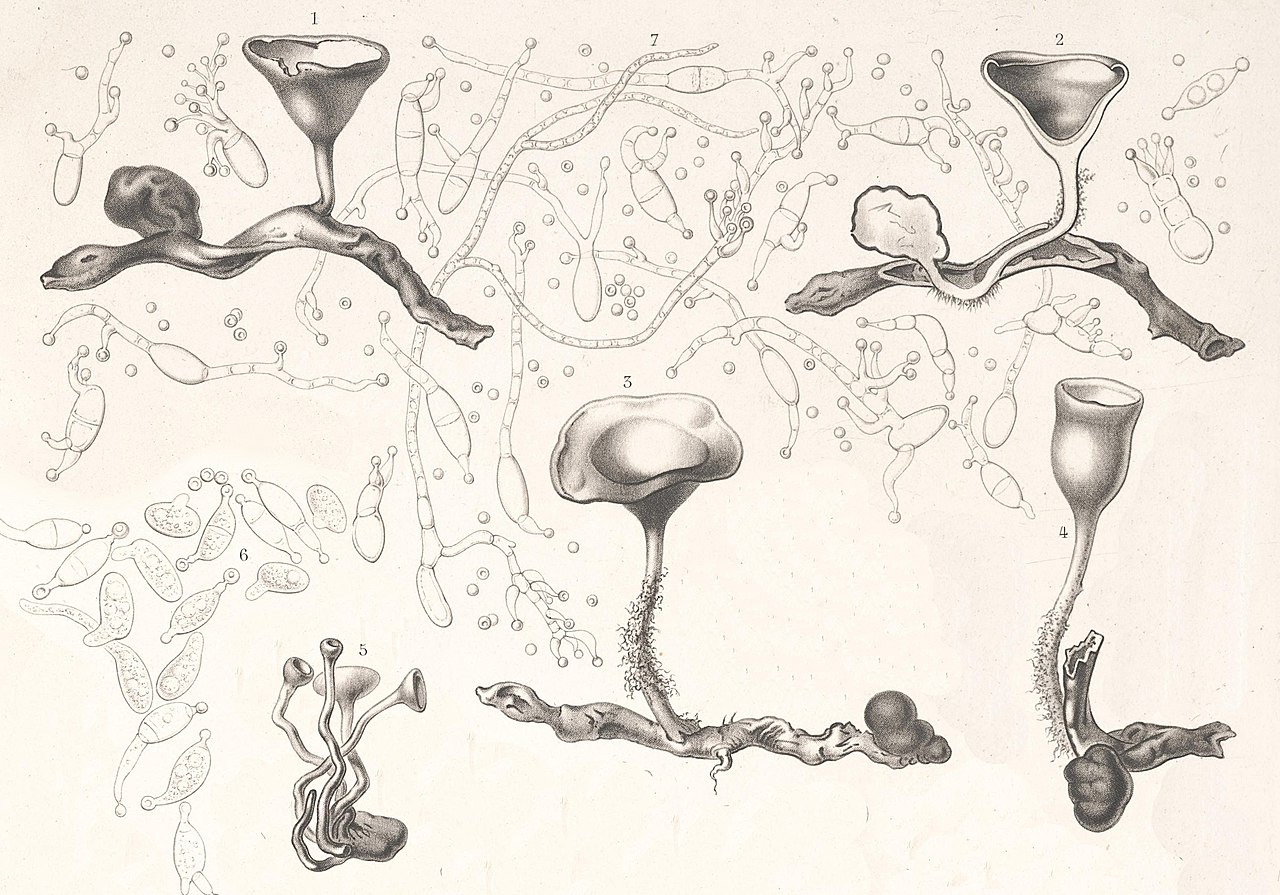
\includegraphics[width=\linewidth]{Figures/PezizaTuberosa.jpg}
%     \caption[Illustration of the fungus Dumontinia tuberosa.]{Illustration of the fungus Dumontinia tuberosa by physician, mycologist, and illustrator Charles Tulasne (1816–1884) in the book Selecta Fungorum Carpologia (1861–65). (Name of the original work: Peziza tuberosa parasite on Anemone nemorosa).}
%     \label{fig:figure-01}
% \end{figure}


\enlargethispage{3\baselineskip}
\begin{figure}[!hb]
\renewcommand\thesubfigure{A.\arabic{subfigure}} % Local change starts here
    \centering
    \begin{subfigure}{0.32\textwidth}
        \centering
        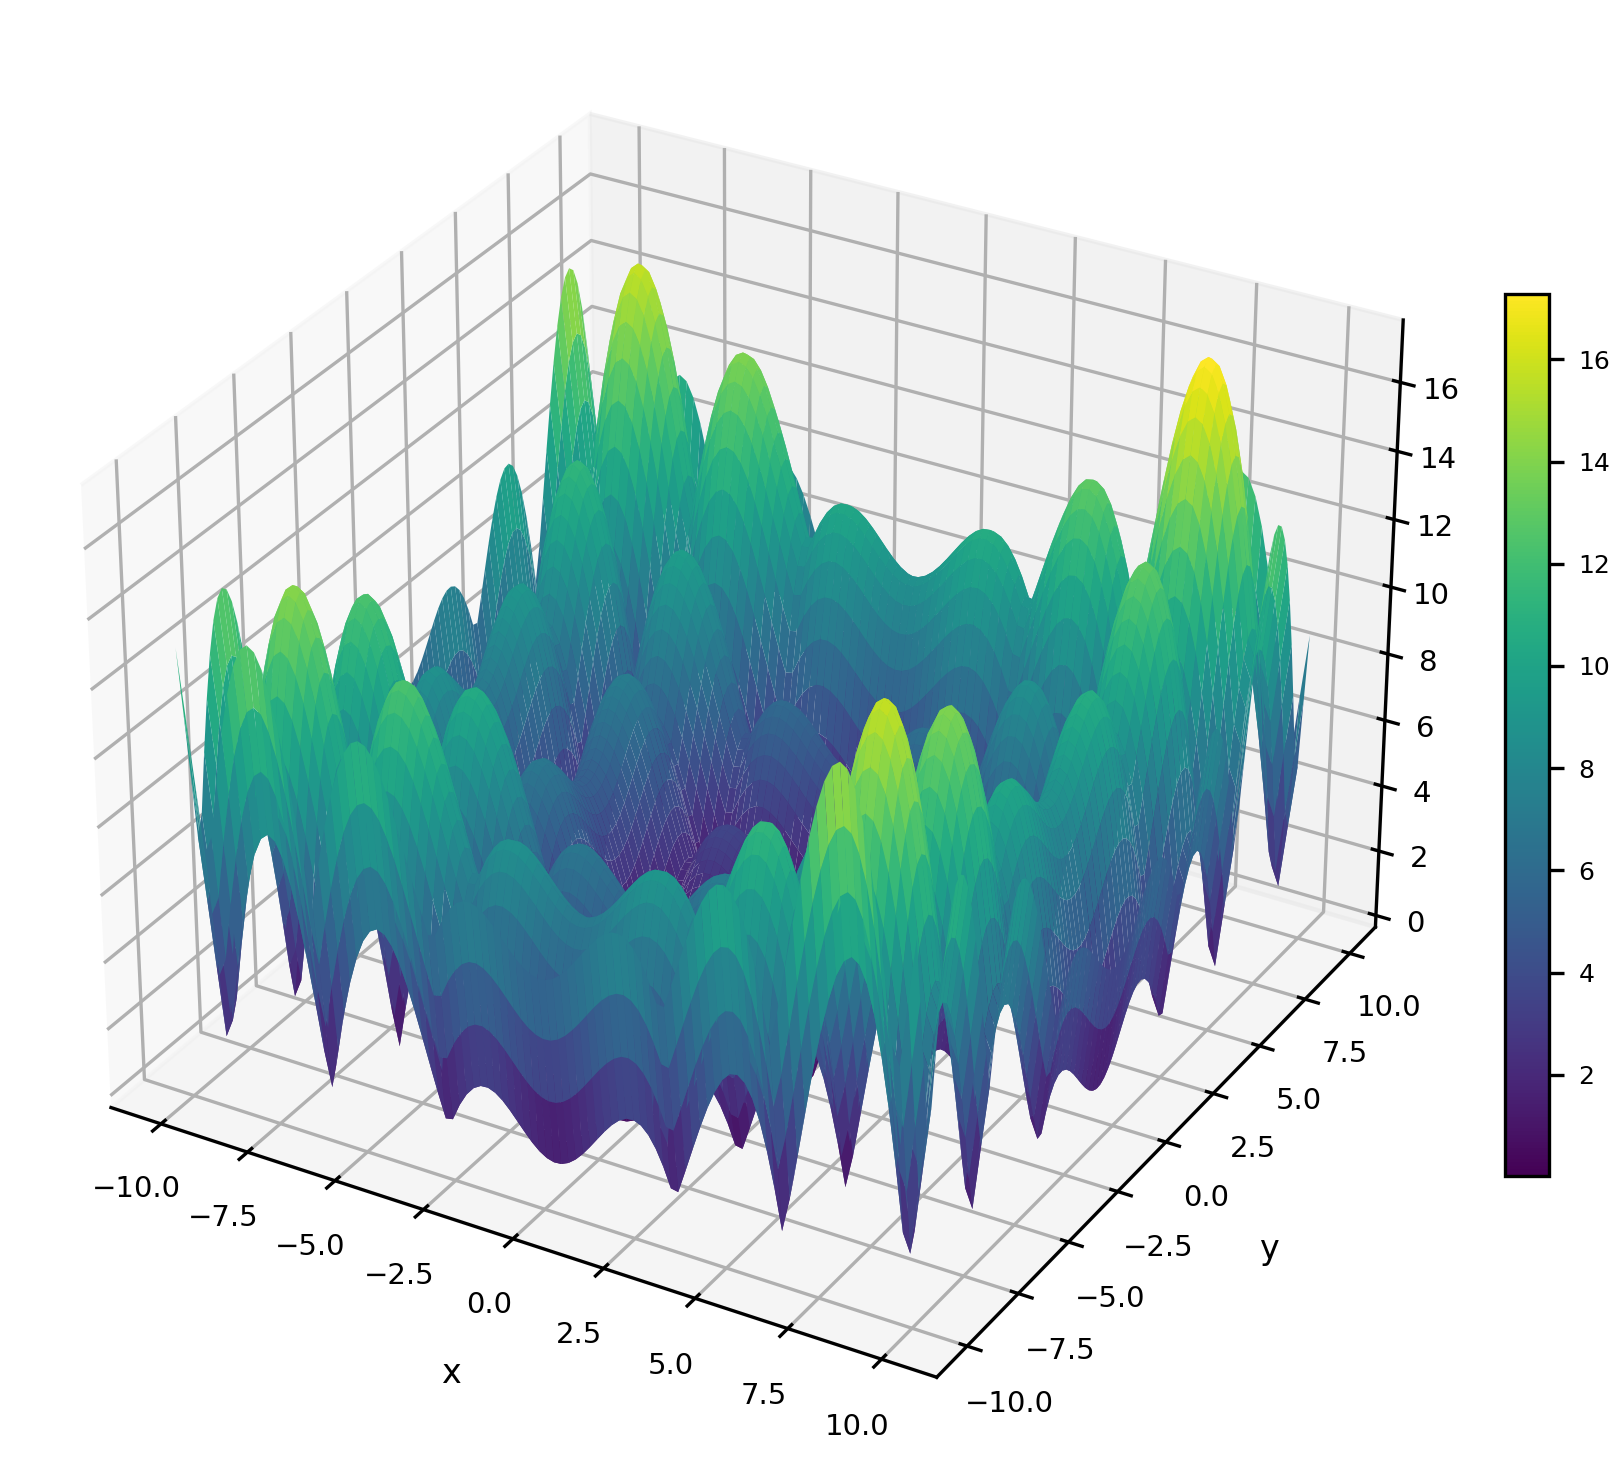
\includegraphics[width=1\textwidth]{Figures/benchmark_plots/Alpine_N1_maximized.png}
        \caption{Alpine N.1}
    \end{subfigure}
    % \hspace{.5cm} % Adjust the space as needed.
    \begin{subfigure}{0.32\textwidth}
        \centering
        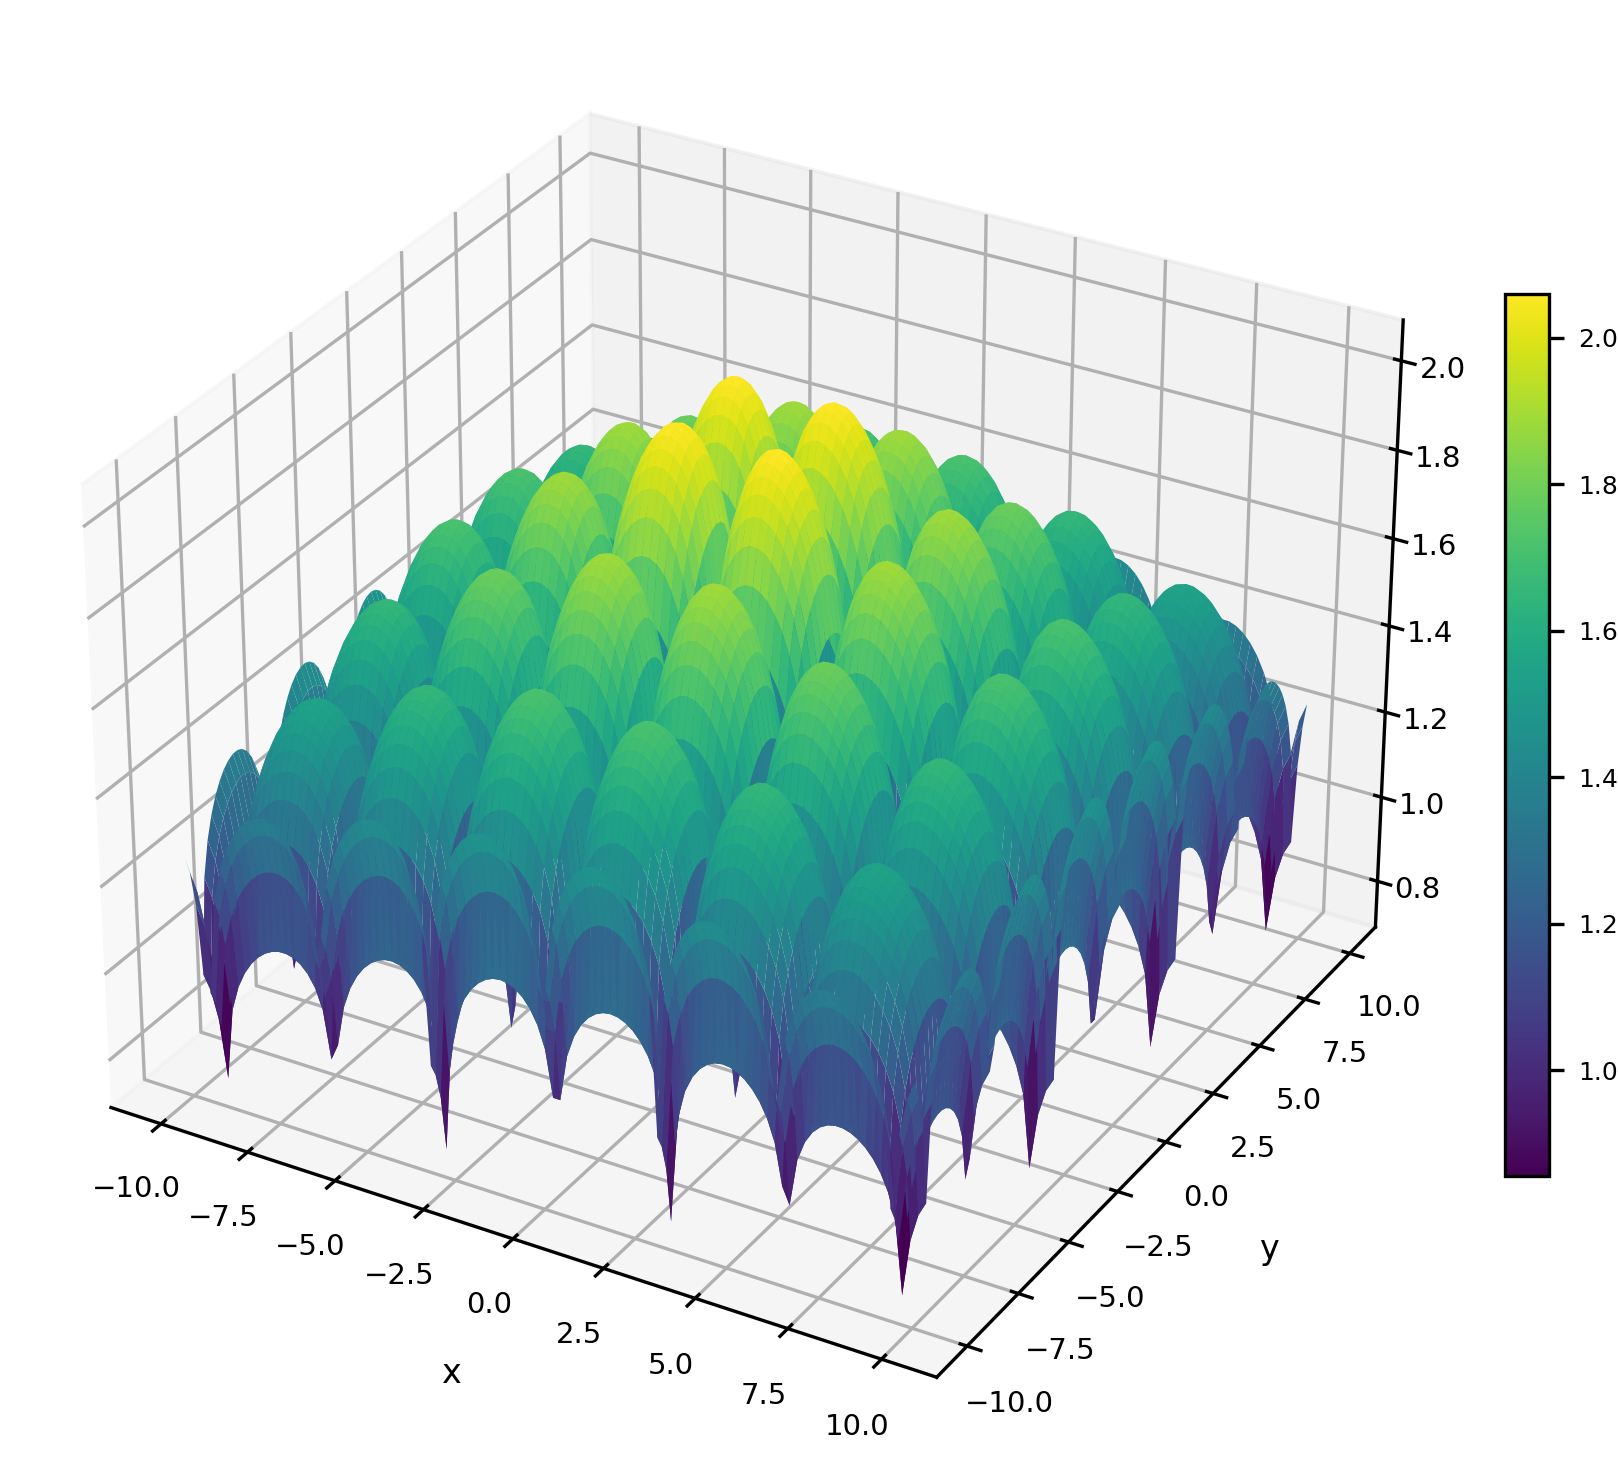
\includegraphics[width=1\textwidth]{Figures/benchmark_plots/Crowned_Cross_maximized.png}
        \caption{Crowned Cross}
    \end{subfigure}
    \begin{subfigure}{0.32\textwidth}
        \centering
        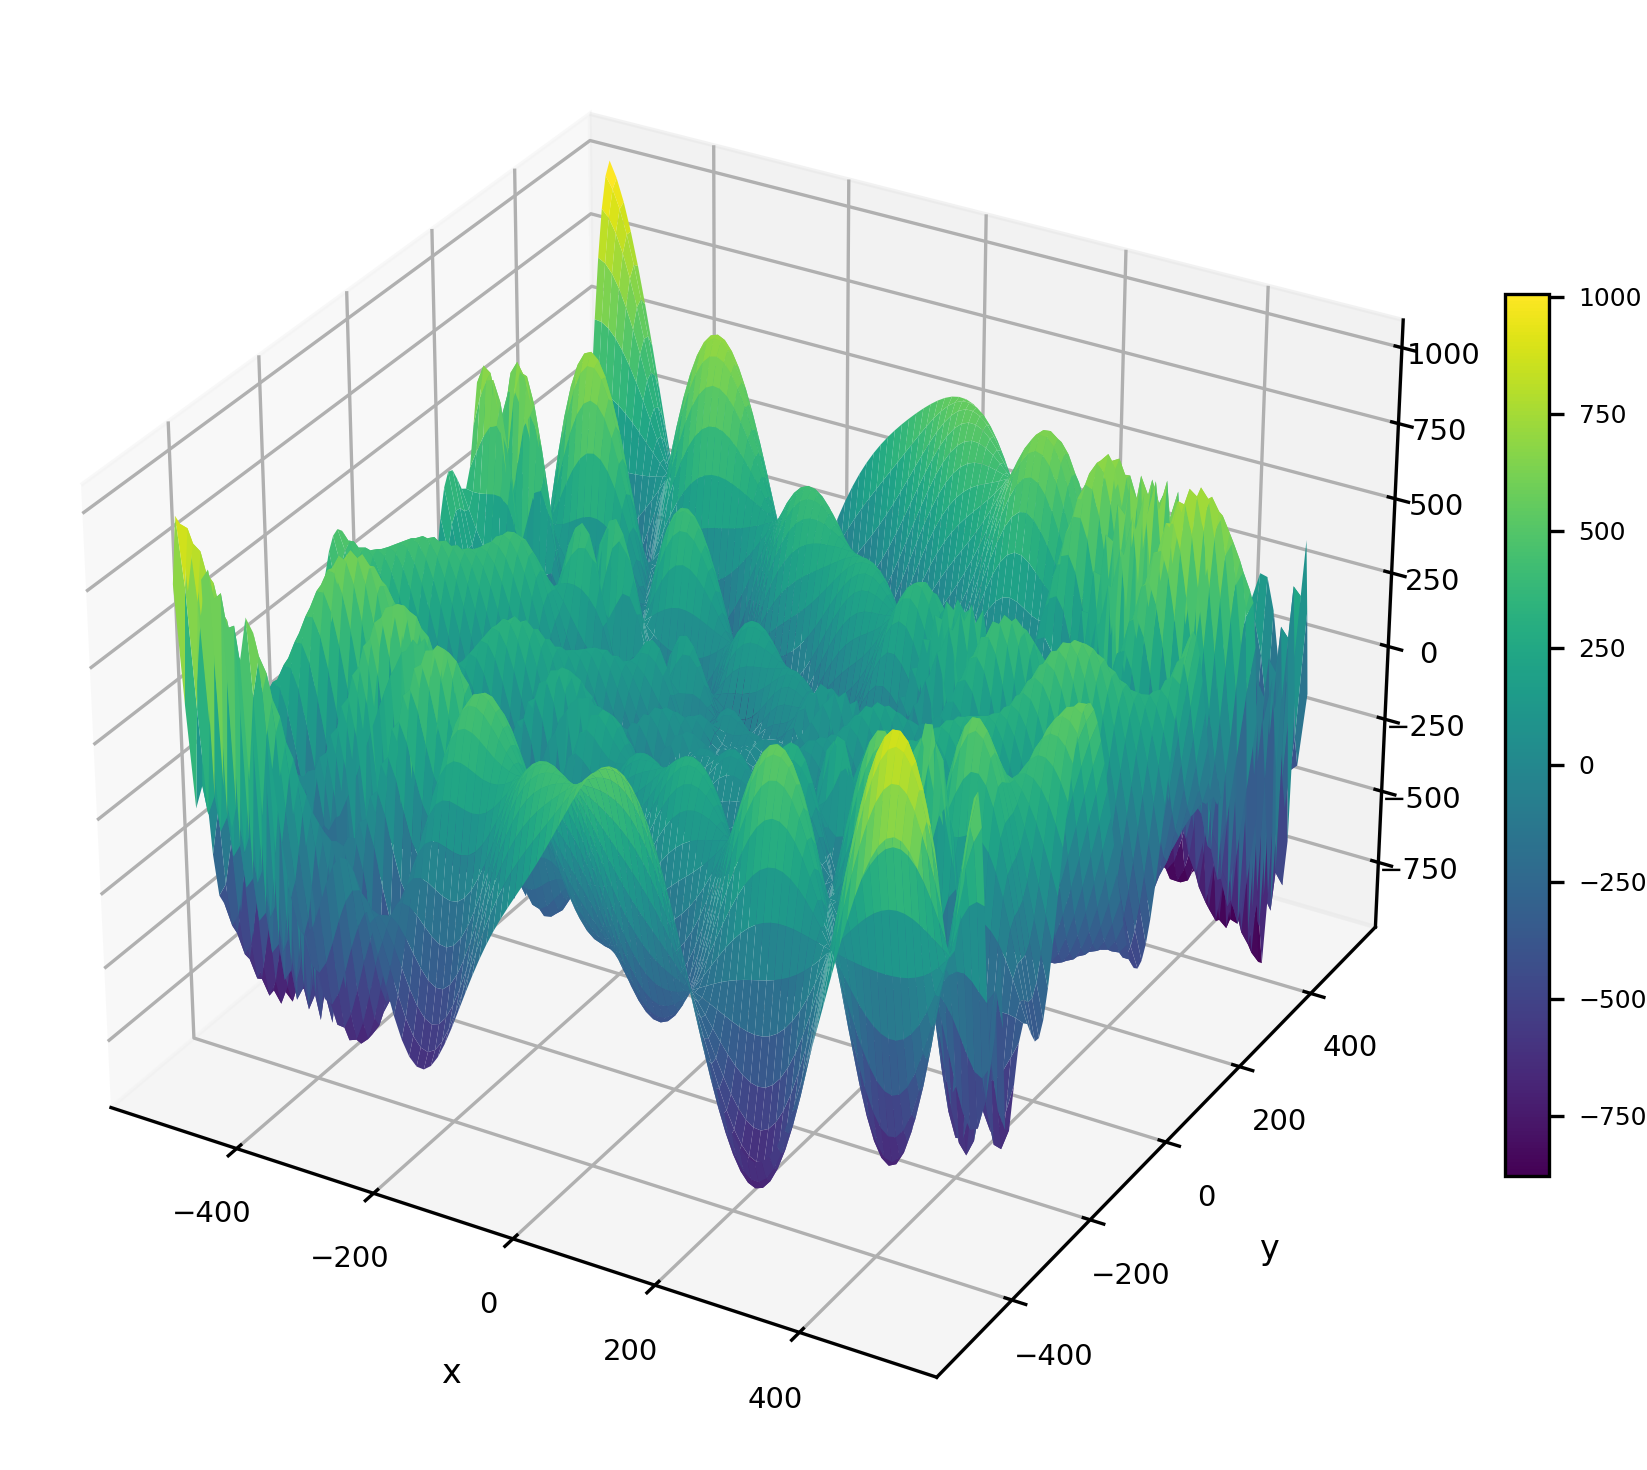
\includegraphics[width=1\textwidth]{Figures/benchmark_plots/Egg_Holder_maximized.png}
        \caption{Egg Holder}
    \end{subfigure}
    % \hspace{.5cm} % Adjust the space as needed.
    \begin{subfigure}{0.32\textwidth}
        \centering
        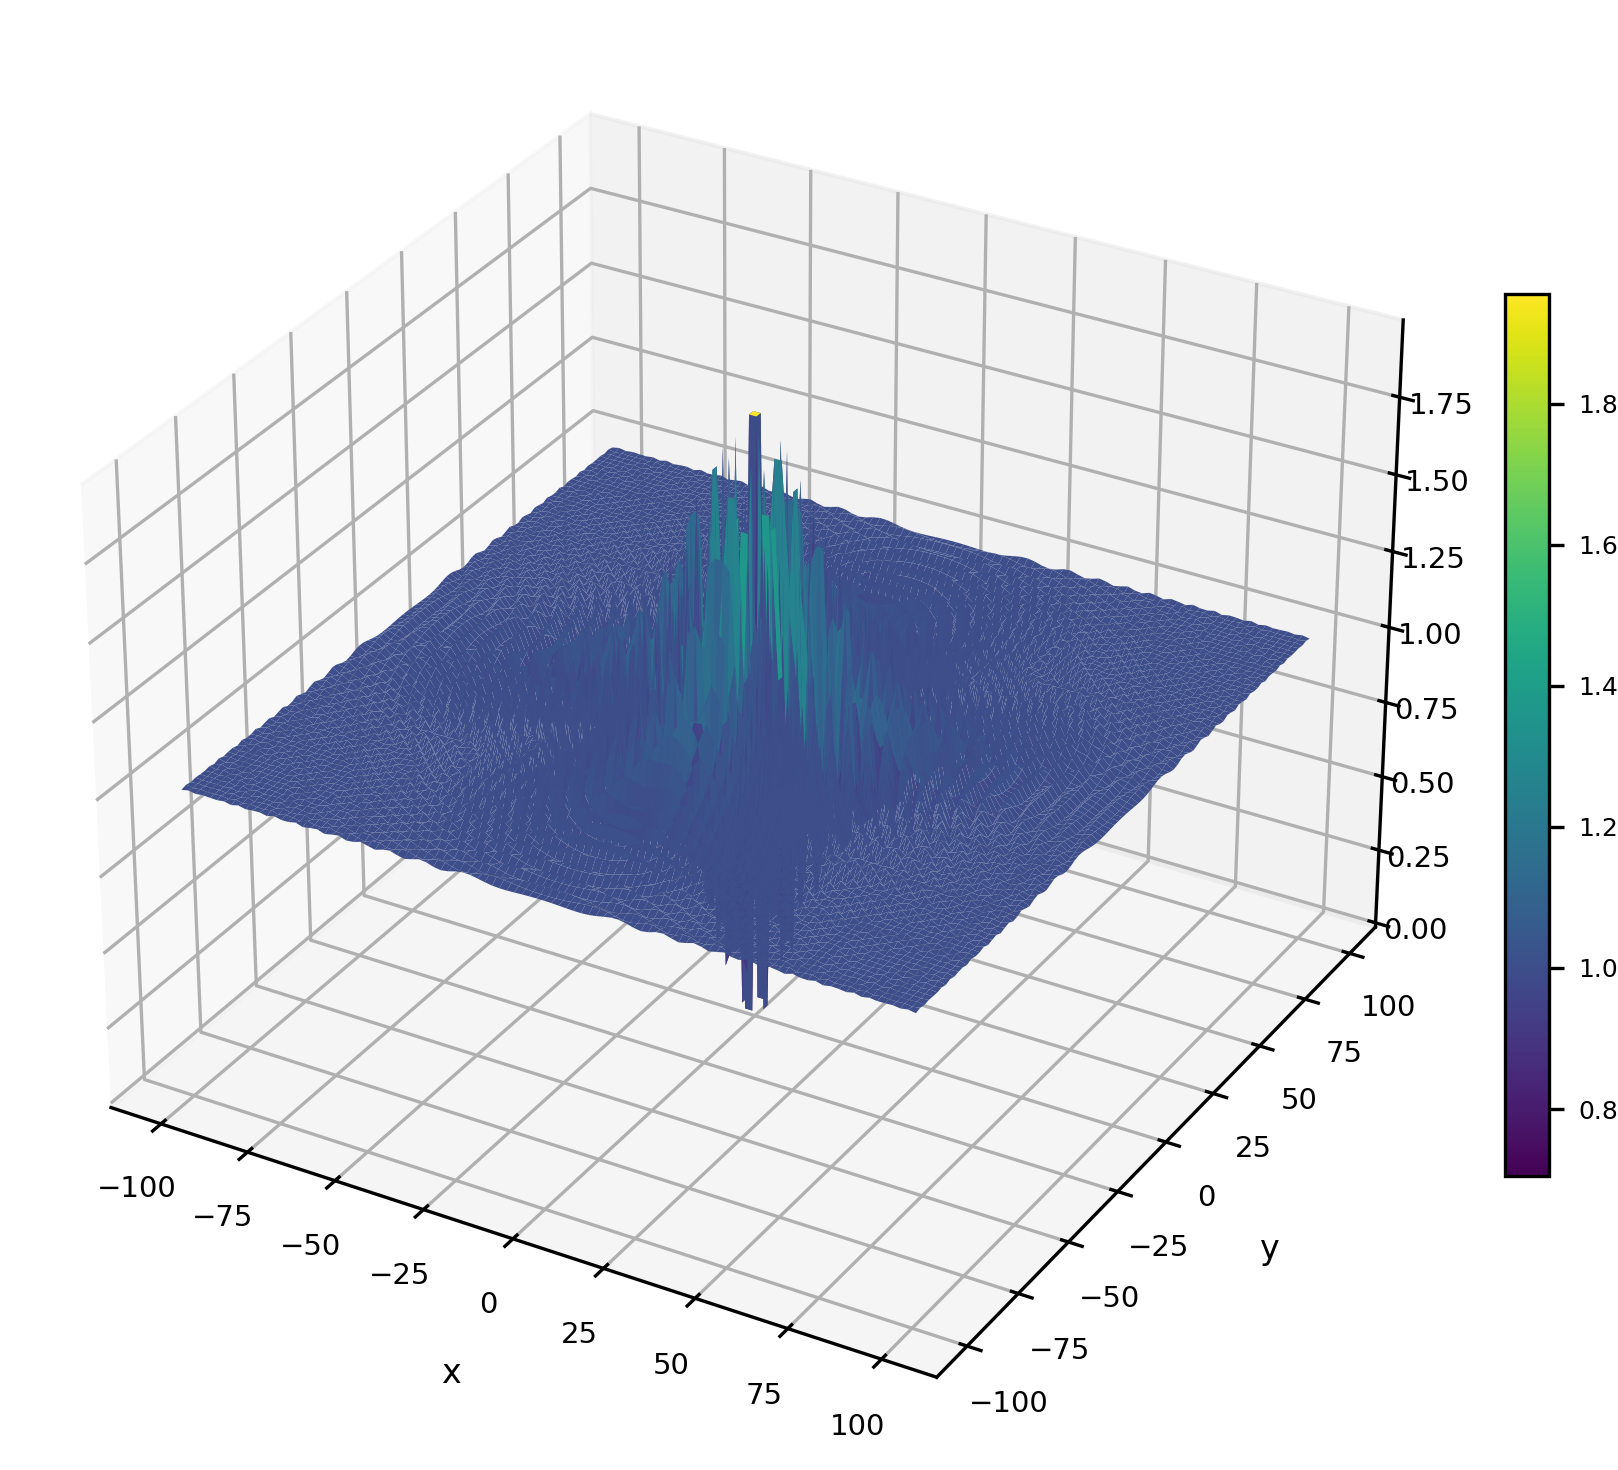
\includegraphics[width=1\textwidth]{Figures/benchmark_plots/Expanded_Shaffer_maximized.png}
        \caption{Expanded Shaffer (F6)}
    \end{subfigure}
        \begin{subfigure}{0.32\textwidth}
        \centering
        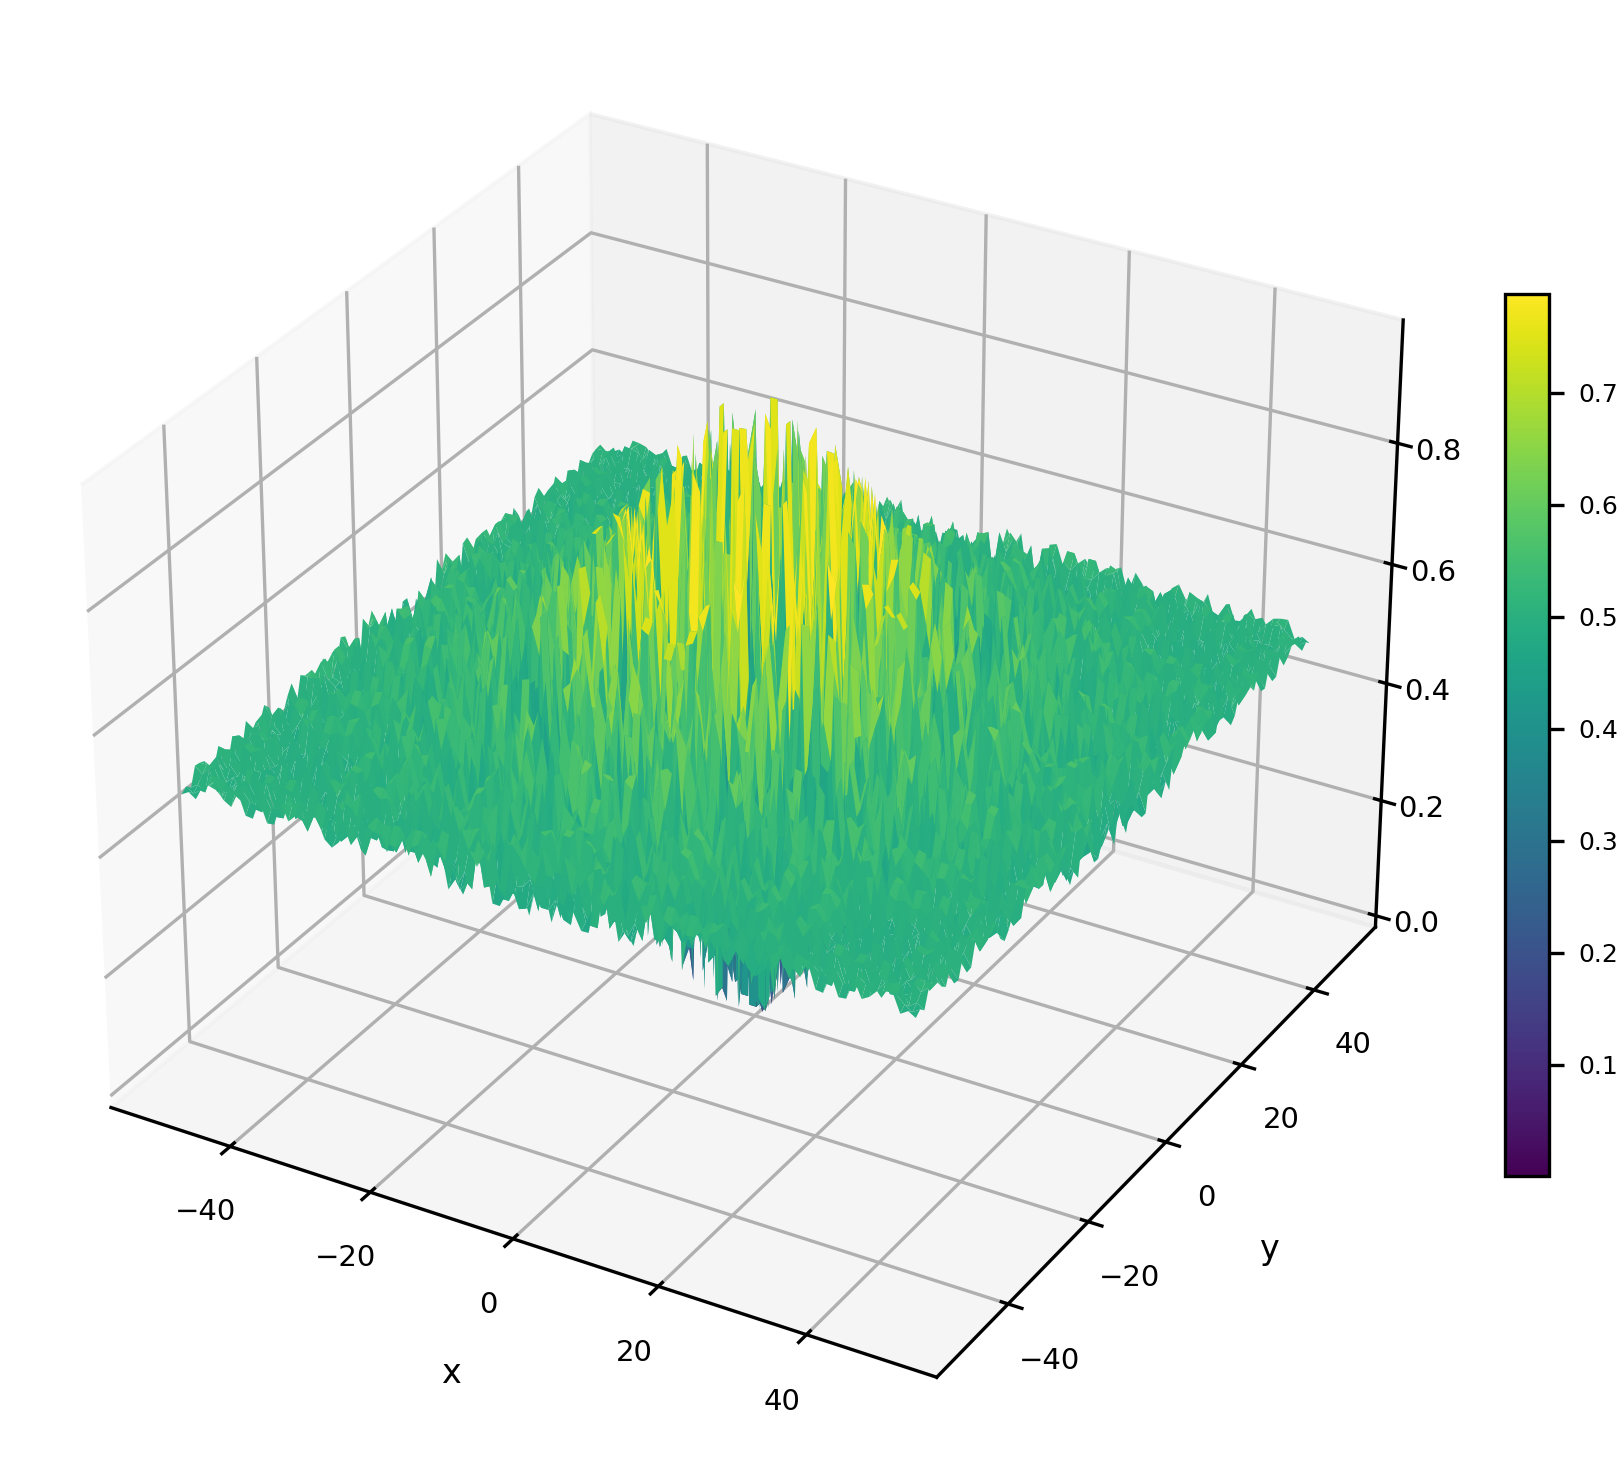
\includegraphics[width=1\textwidth]{Figures/benchmark_plots/Generalized_Schaffer_N1_maximized.png}
        \caption{Generalized Schaffer N1}
    \end{subfigure}
        \begin{subfigure}{0.32\textwidth}
        \centering
        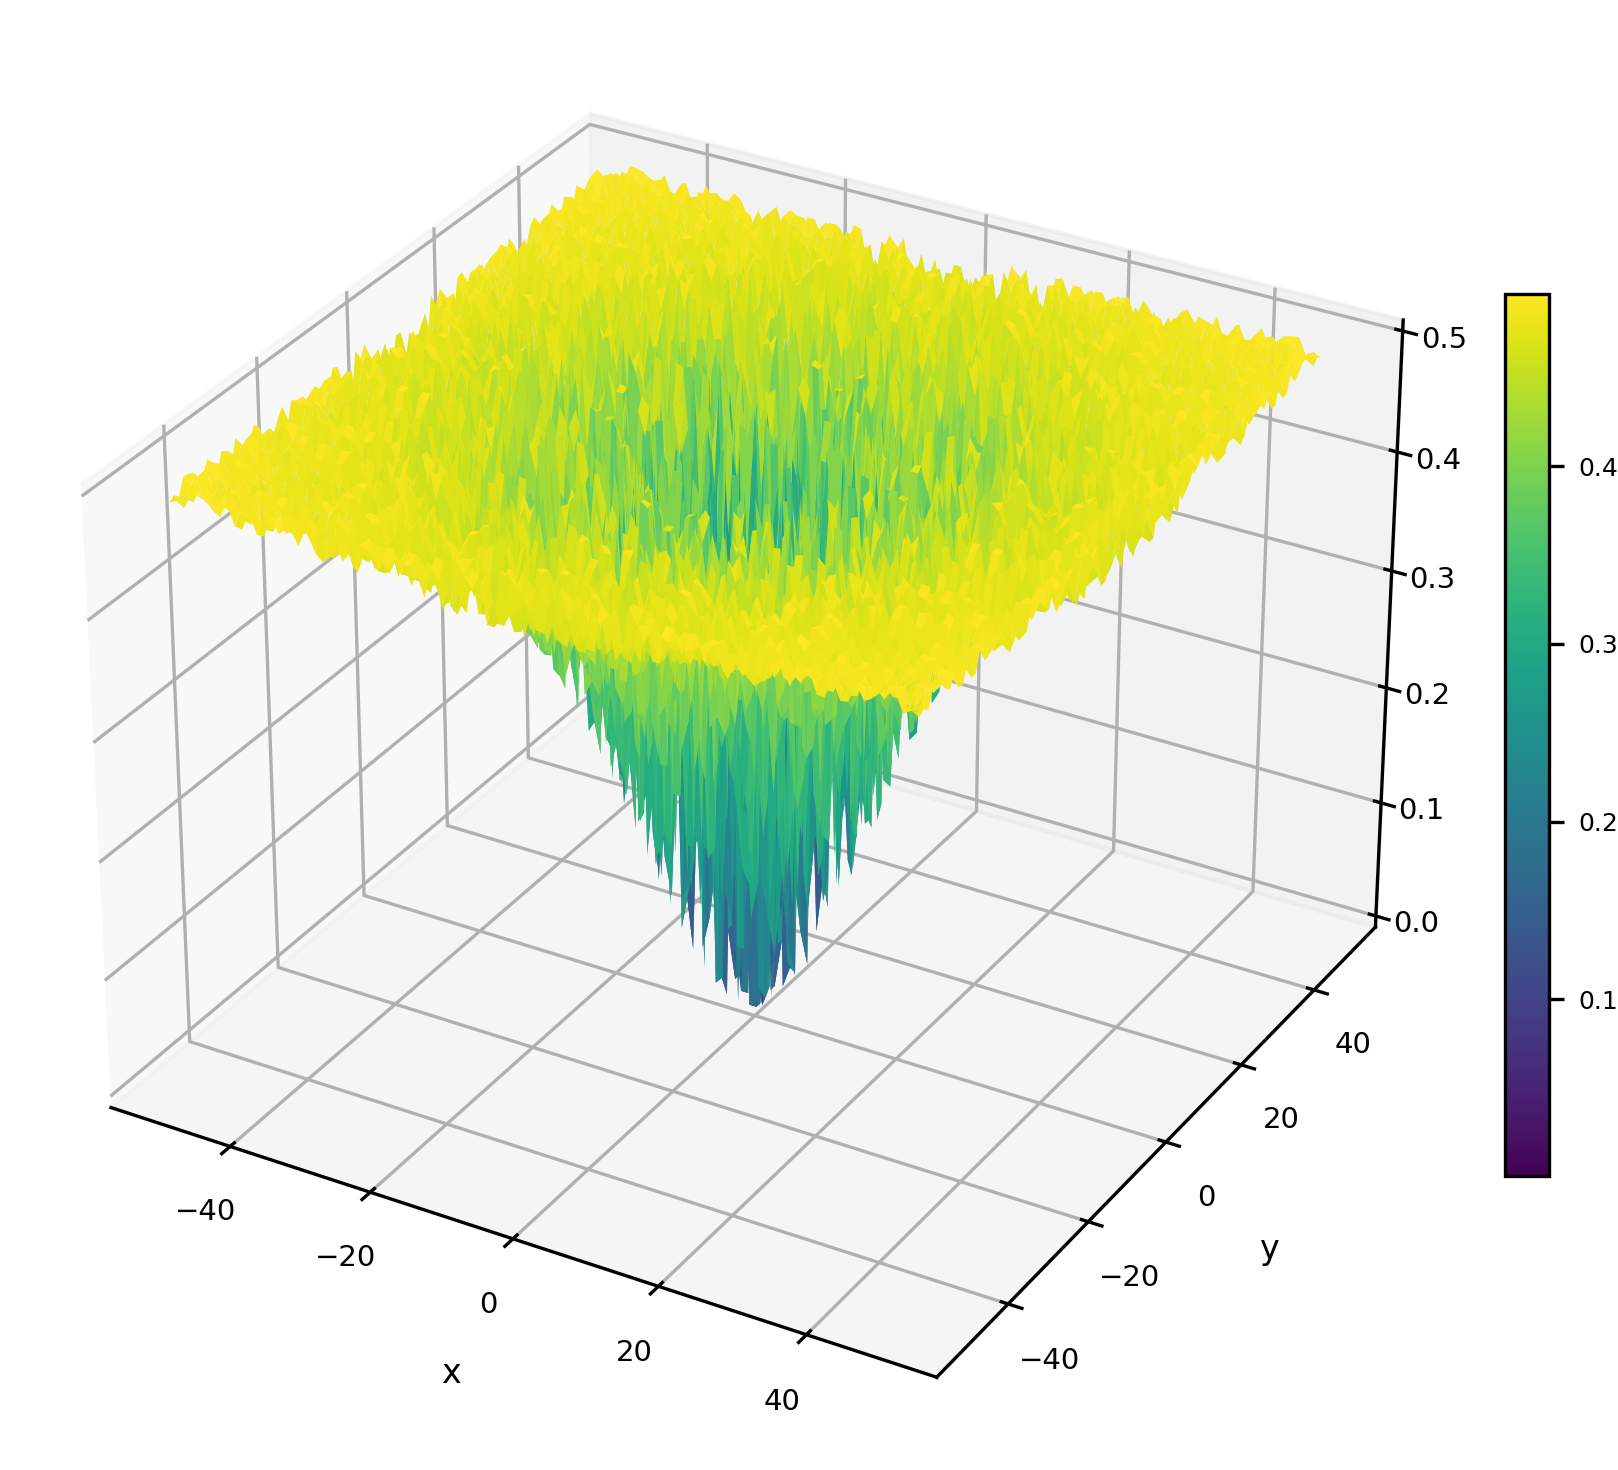
\includegraphics[width=1\textwidth]{Figures/benchmark_plots/Generalized_Schaffer_N2_maximized.png}
        \caption{Generalized Schaffer N2}
    \end{subfigure}
        \begin{subfigure}{0.32\textwidth}
        \centering
        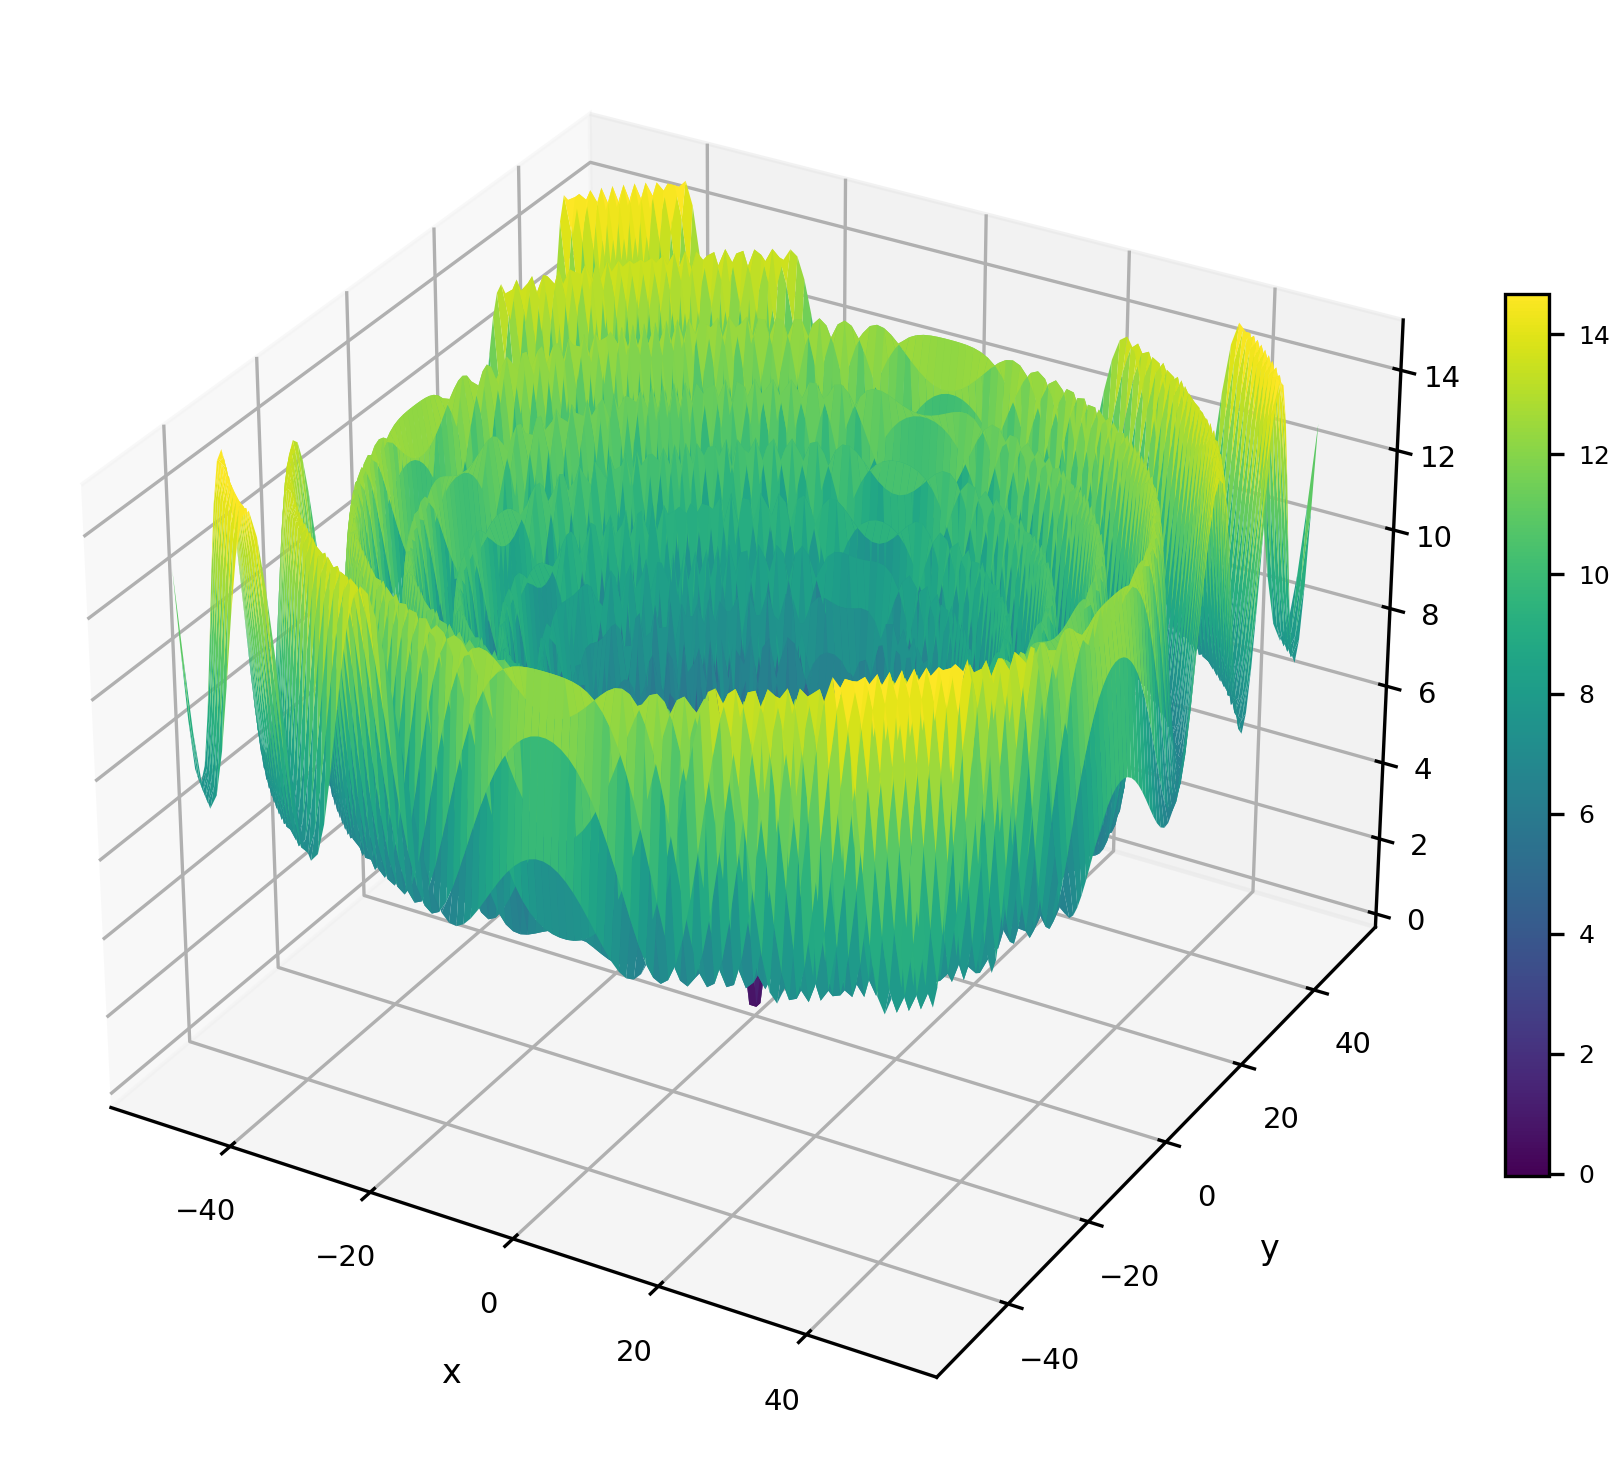
\includegraphics[width=1\textwidth]{Figures/benchmark_plots/Generalized_Schaffer_N3_maximized.png}
        \caption{Generalized Schaffer N3}
    \end{subfigure}
      \begin{subfigure}{0.32\textwidth}
        \centering
        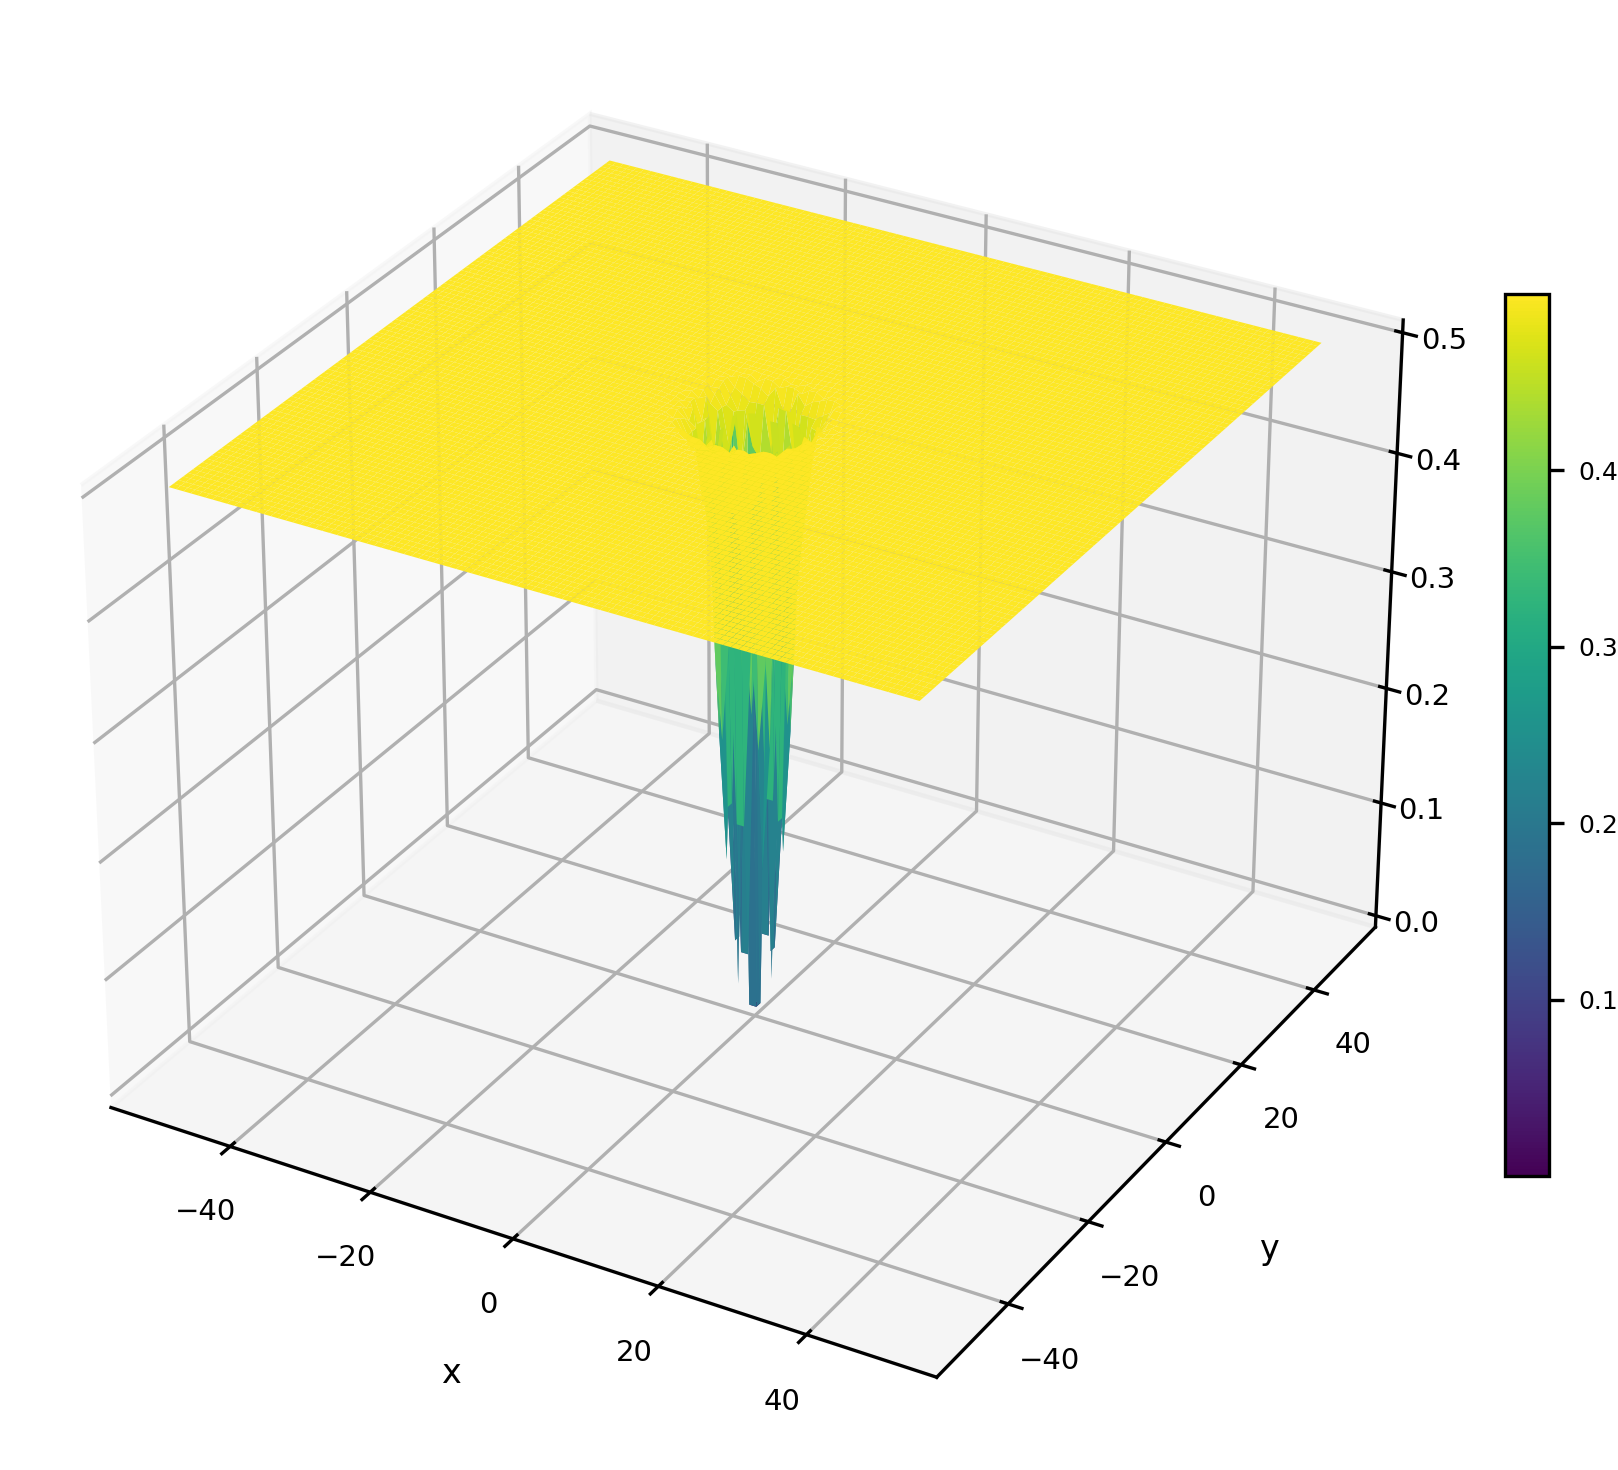
\includegraphics[width=1\textwidth]{Figures/benchmark_plots/Generalized_Schaffer_N4_maximized.png}
        \caption{Generalized Schaffer N4}
    \end{subfigure}
        \begin{subfigure}{0.32\textwidth}
        \centering
        \includegraphics[width=1\textwidth]{Figures/benchmark_plots/Generalized_Schmidt–Vetters_maximized.png}
        \caption{Schmidt–Vetters}
    \end{subfigure}
    \caption[Visualizations of benchmark problem landscapes]{Two-dimensional visualizations of benchmark problem landscapes.}
\end{figure}


\begin{figure}[p]\ContinuedFloat
\renewcommand\thesubfigure{A.\arabic{subfigure}} % Local change starts here
    \centering
    \begin{subfigure}{0.32\textwidth}
        \centering
        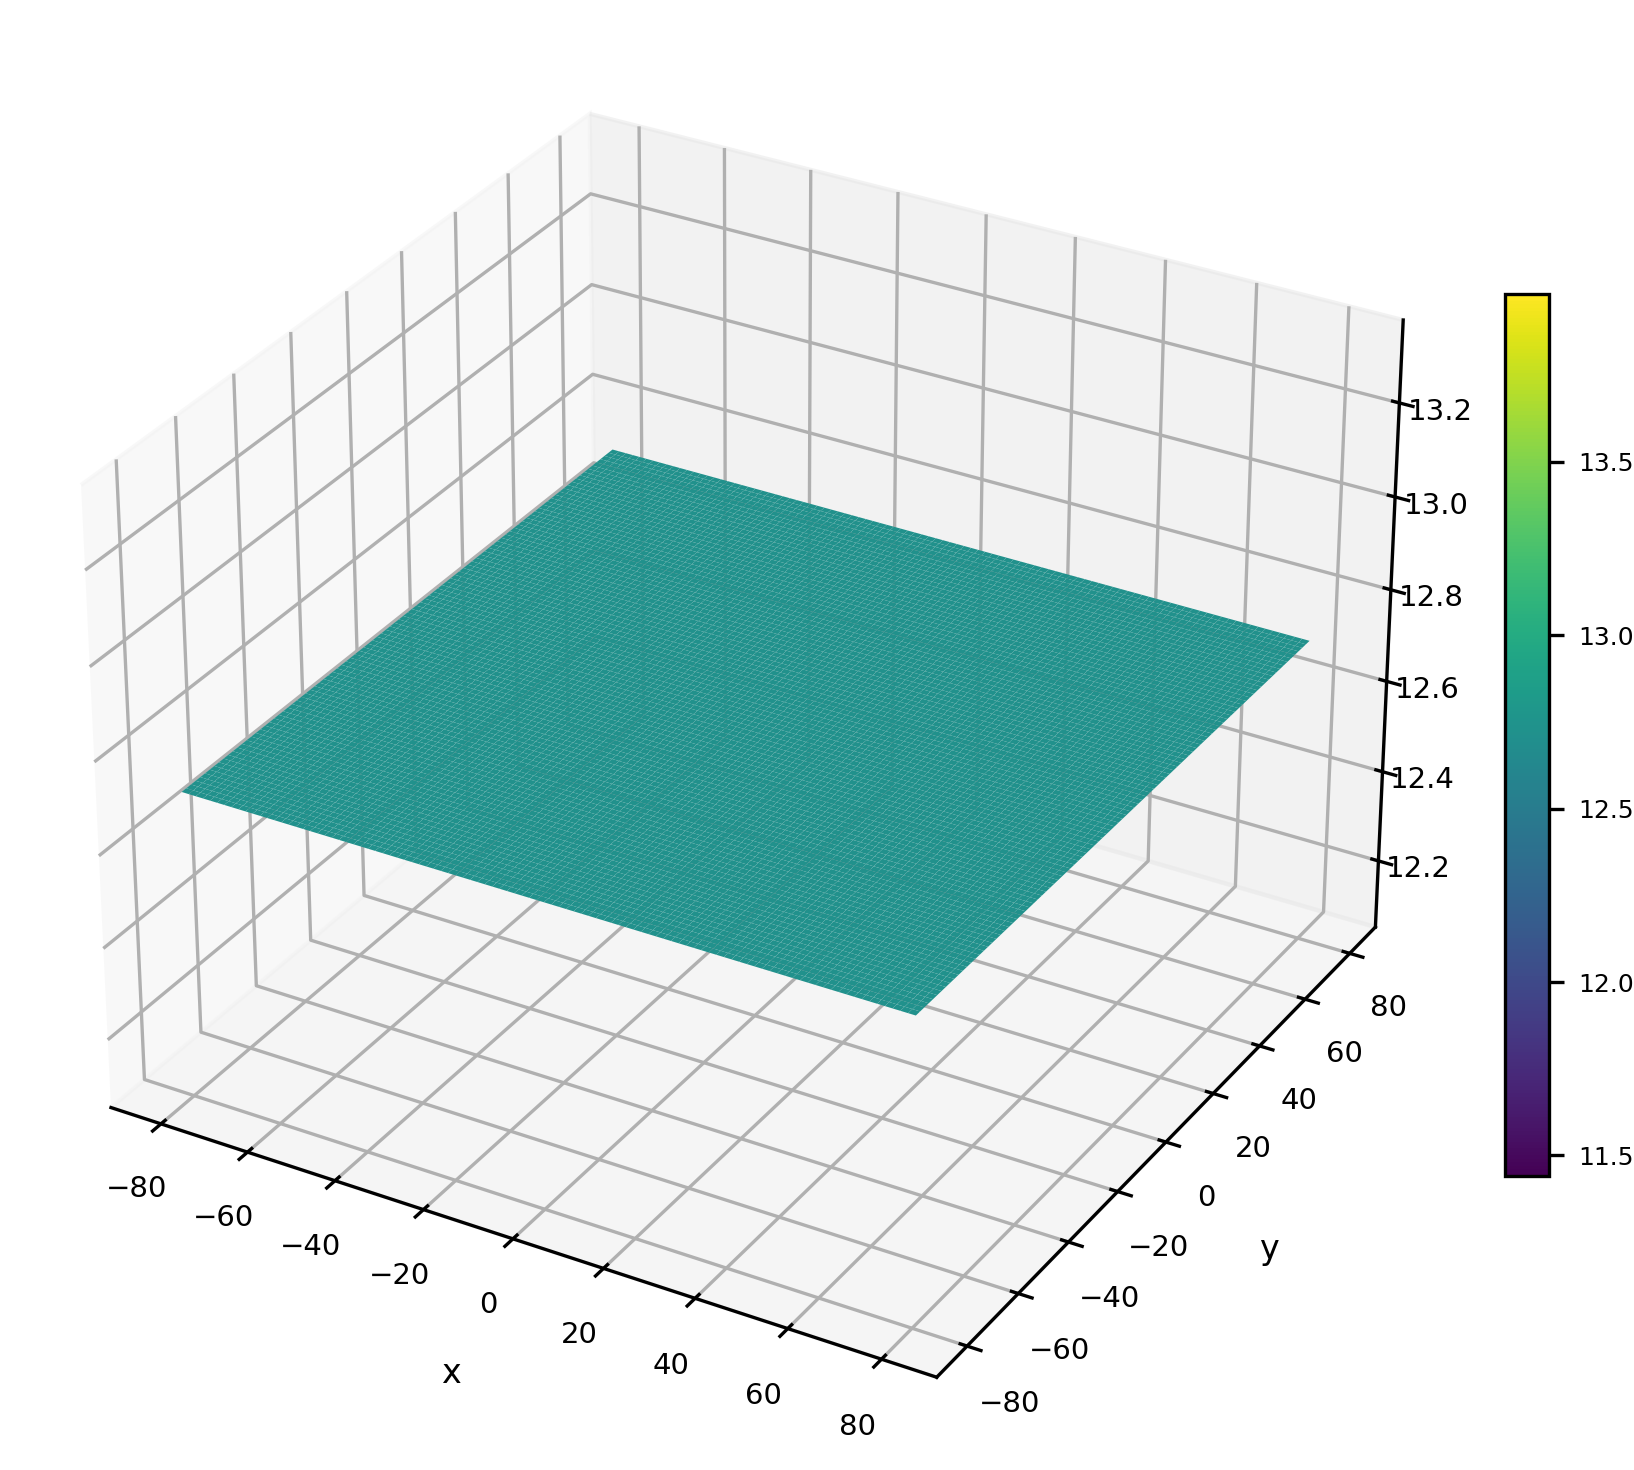
\includegraphics[width=1\textwidth]{Figures/benchmark_plots/Lennard_Jones_Minimum_Energy_Cluster_maximized.png}
        \caption{Lennard‑Jones}
    \end{subfigure}
    \begin{subfigure}{0.32\textwidth}
        \centering
        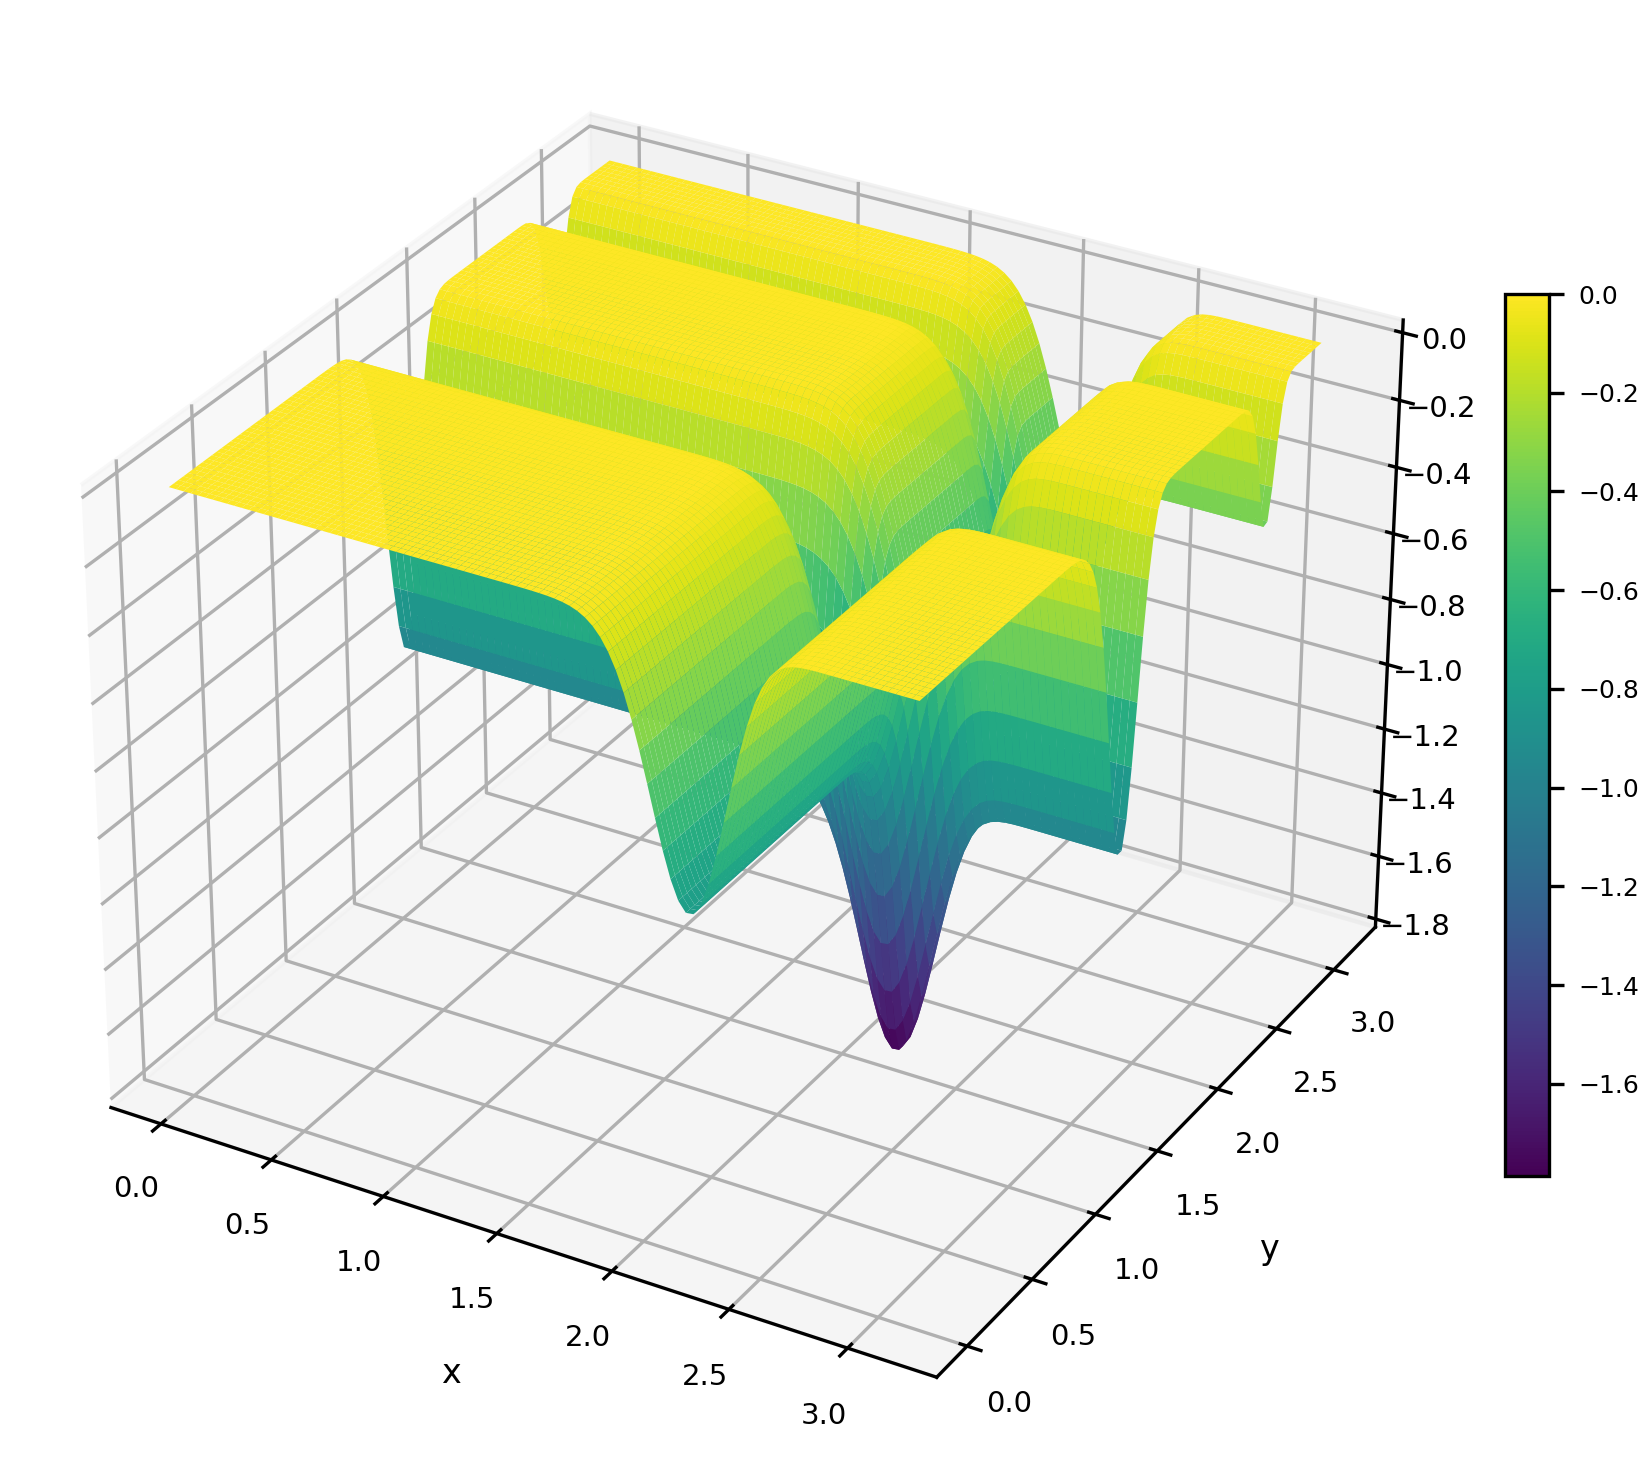
\includegraphics[width=1\textwidth]{Figures/benchmark_plots/Michalewicz_maximized.png}
        \caption{Michalewicz}
    \end{subfigure}
    % \hspace{.5cm} % Adjust the space as needed.
    \begin{subfigure}{0.32\textwidth}
        \centering
        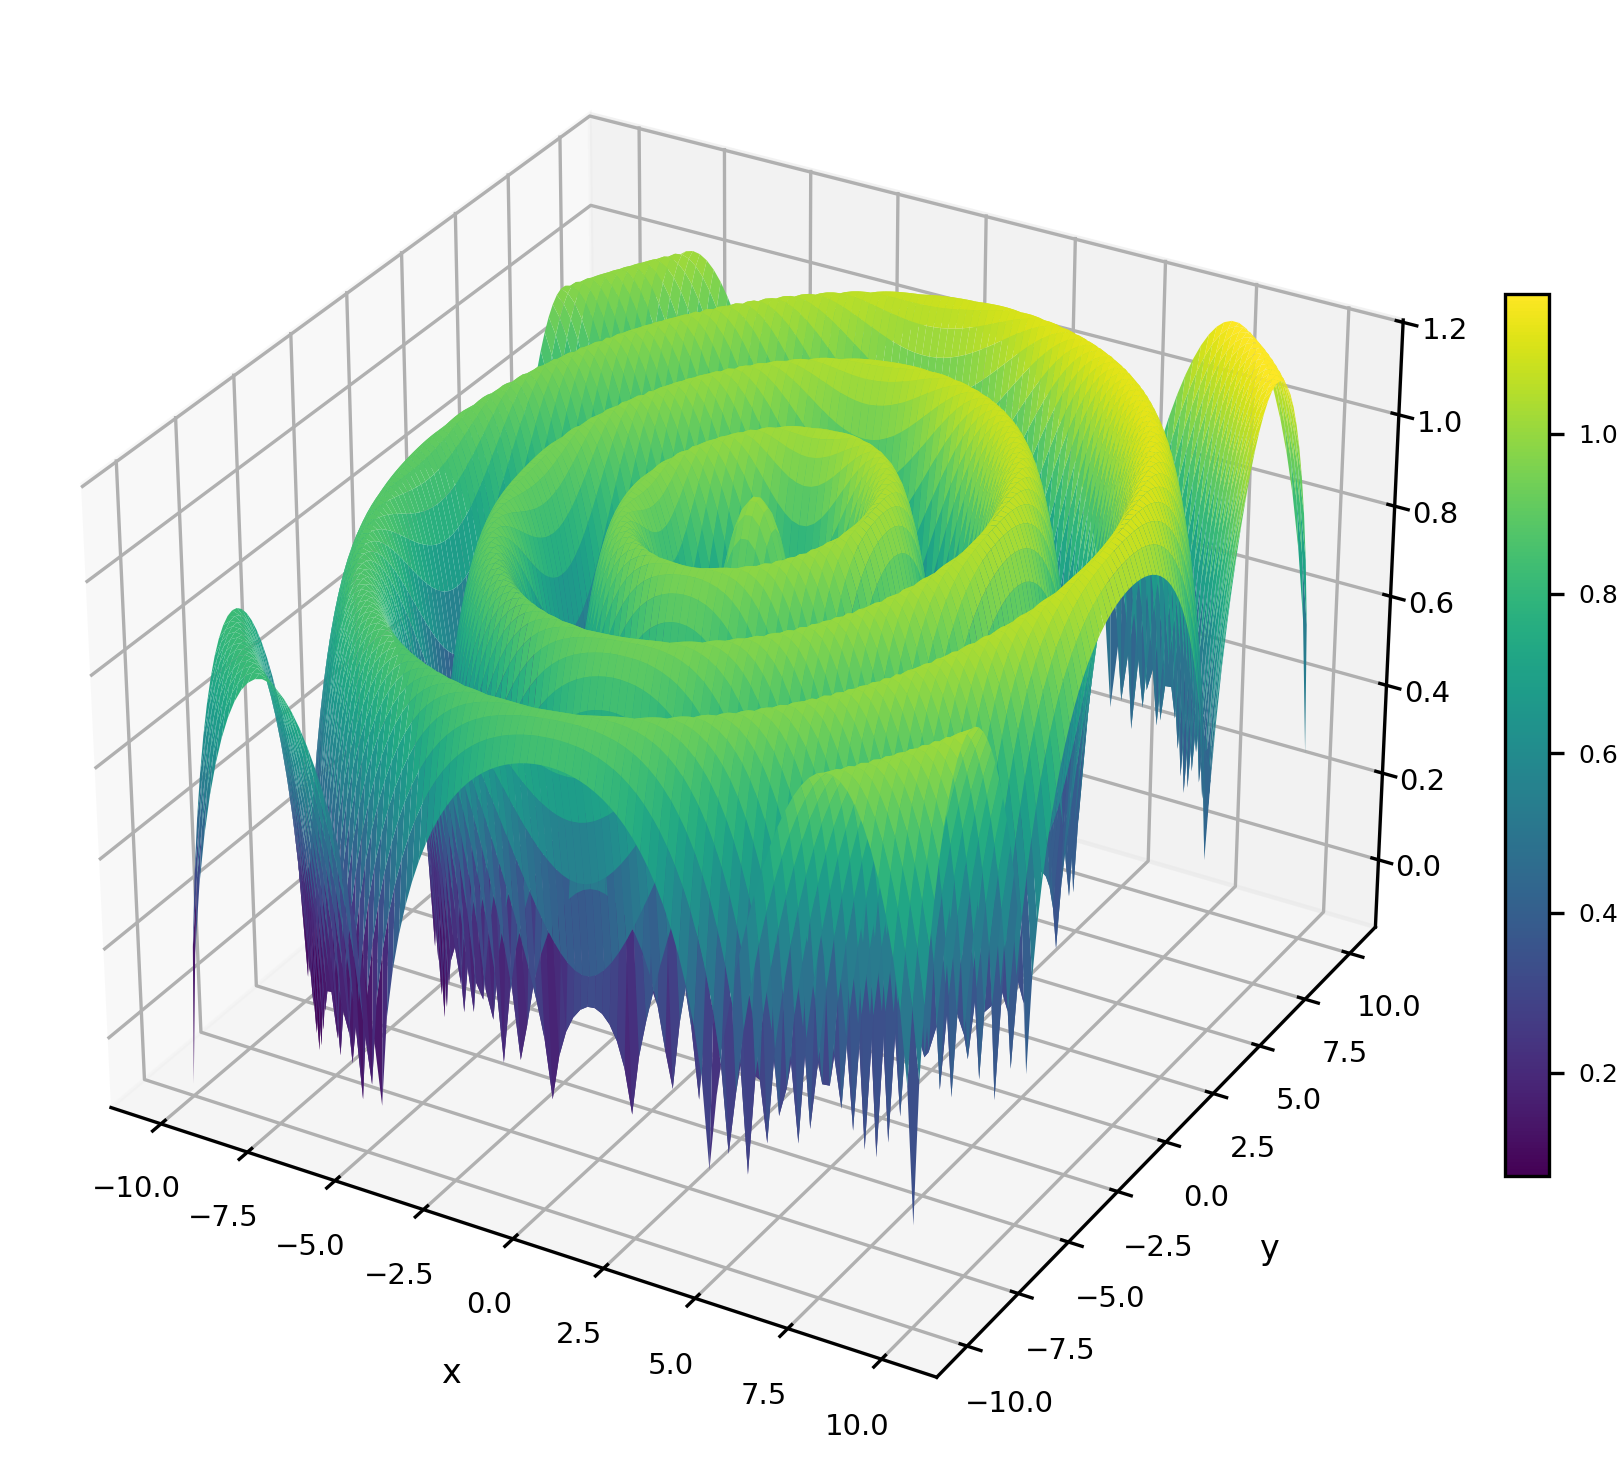
\includegraphics[width=1\textwidth]{Figures/benchmark_plots/Mishra_N3_maximized.png}
        \caption{Mishra 03}
    \end{subfigure}
    \begin{subfigure}{0.48\textwidth}
        \centering
        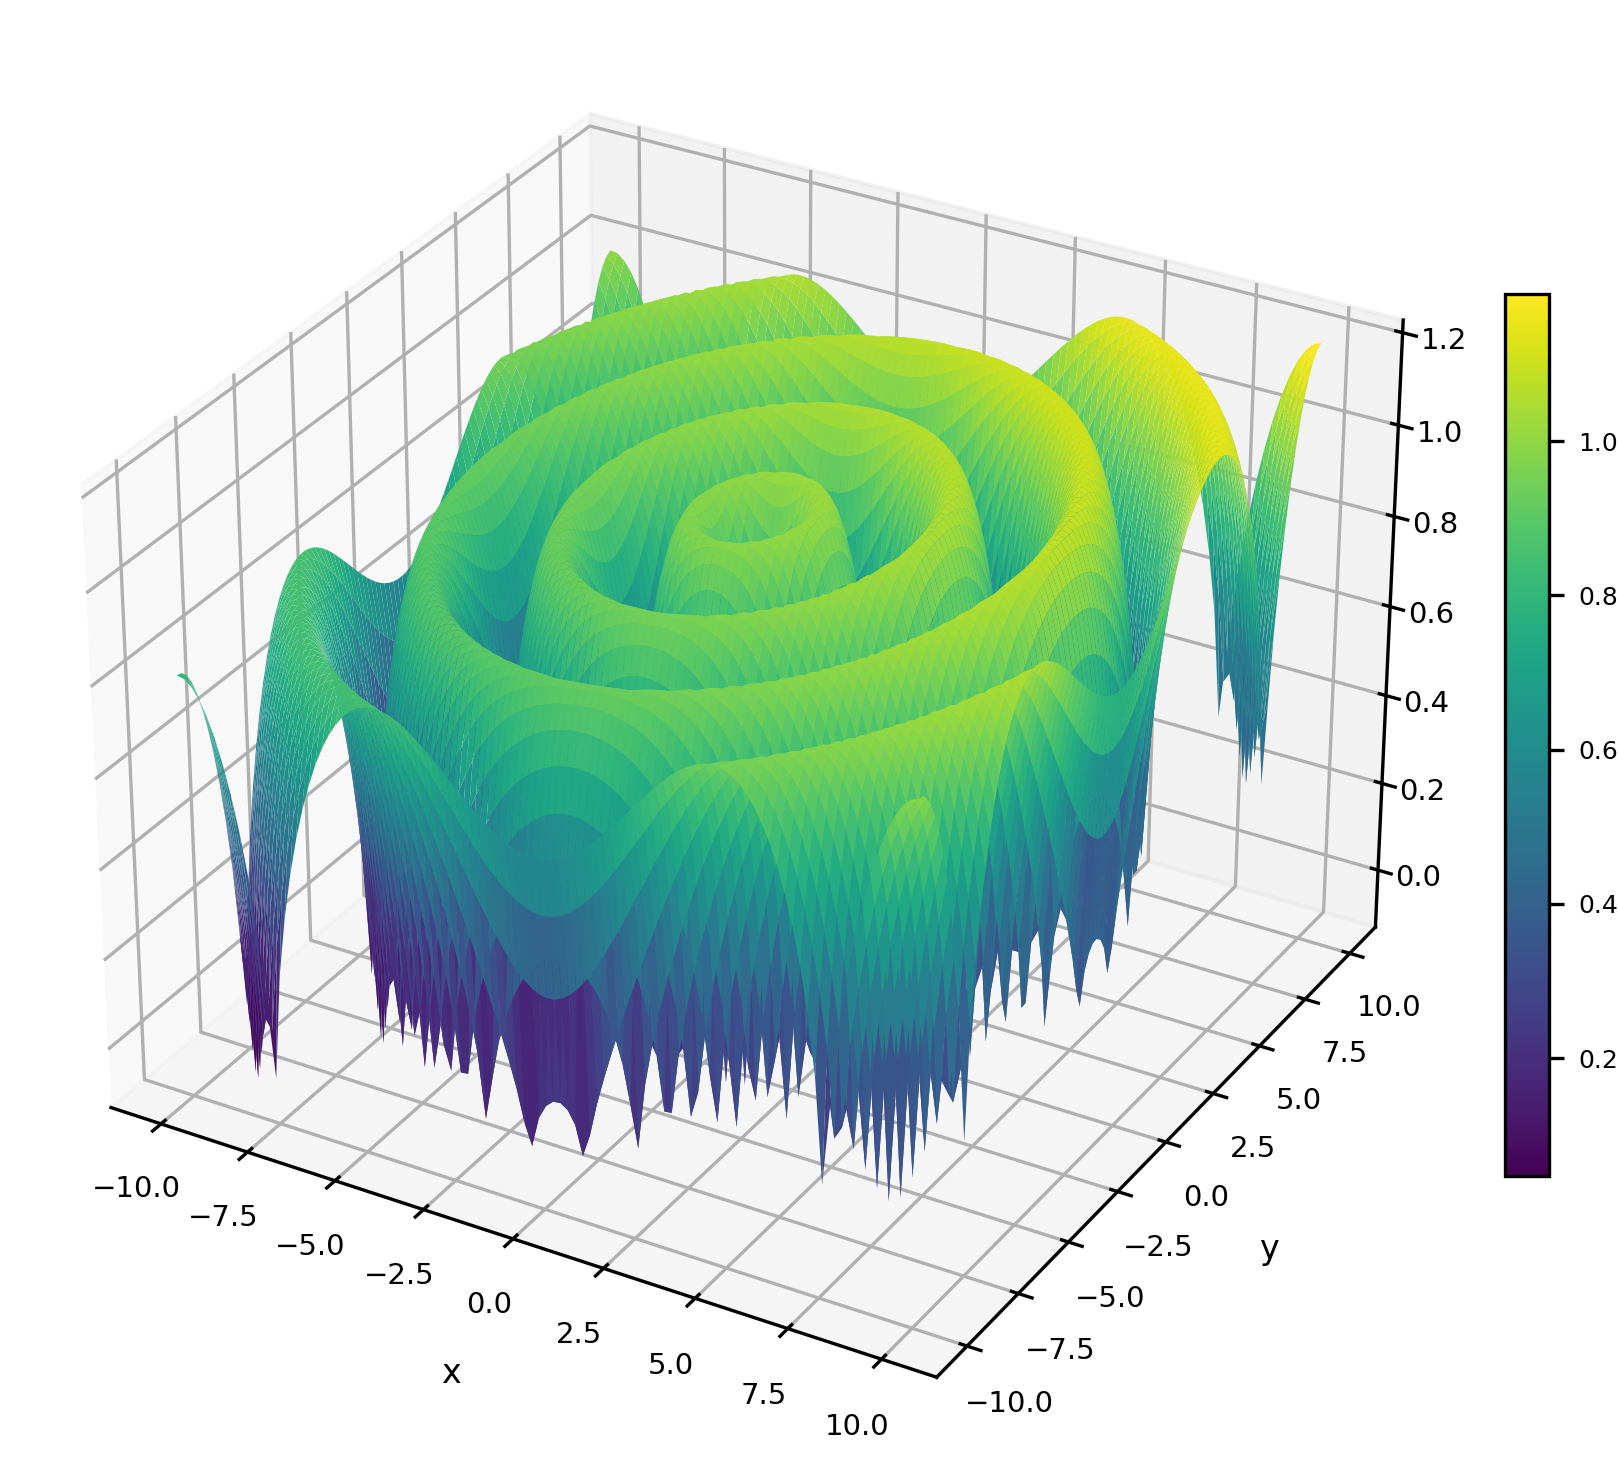
\includegraphics[width=1\textwidth]{Figures/benchmark_plots/Mishra_N4_maximized.png}
        \caption{Mishra 04}
    \end{subfigure}
    % \hspace{.5cm} % Adjust the space as needed.
    \begin{subfigure}{0.48\textwidth}
        \centering
        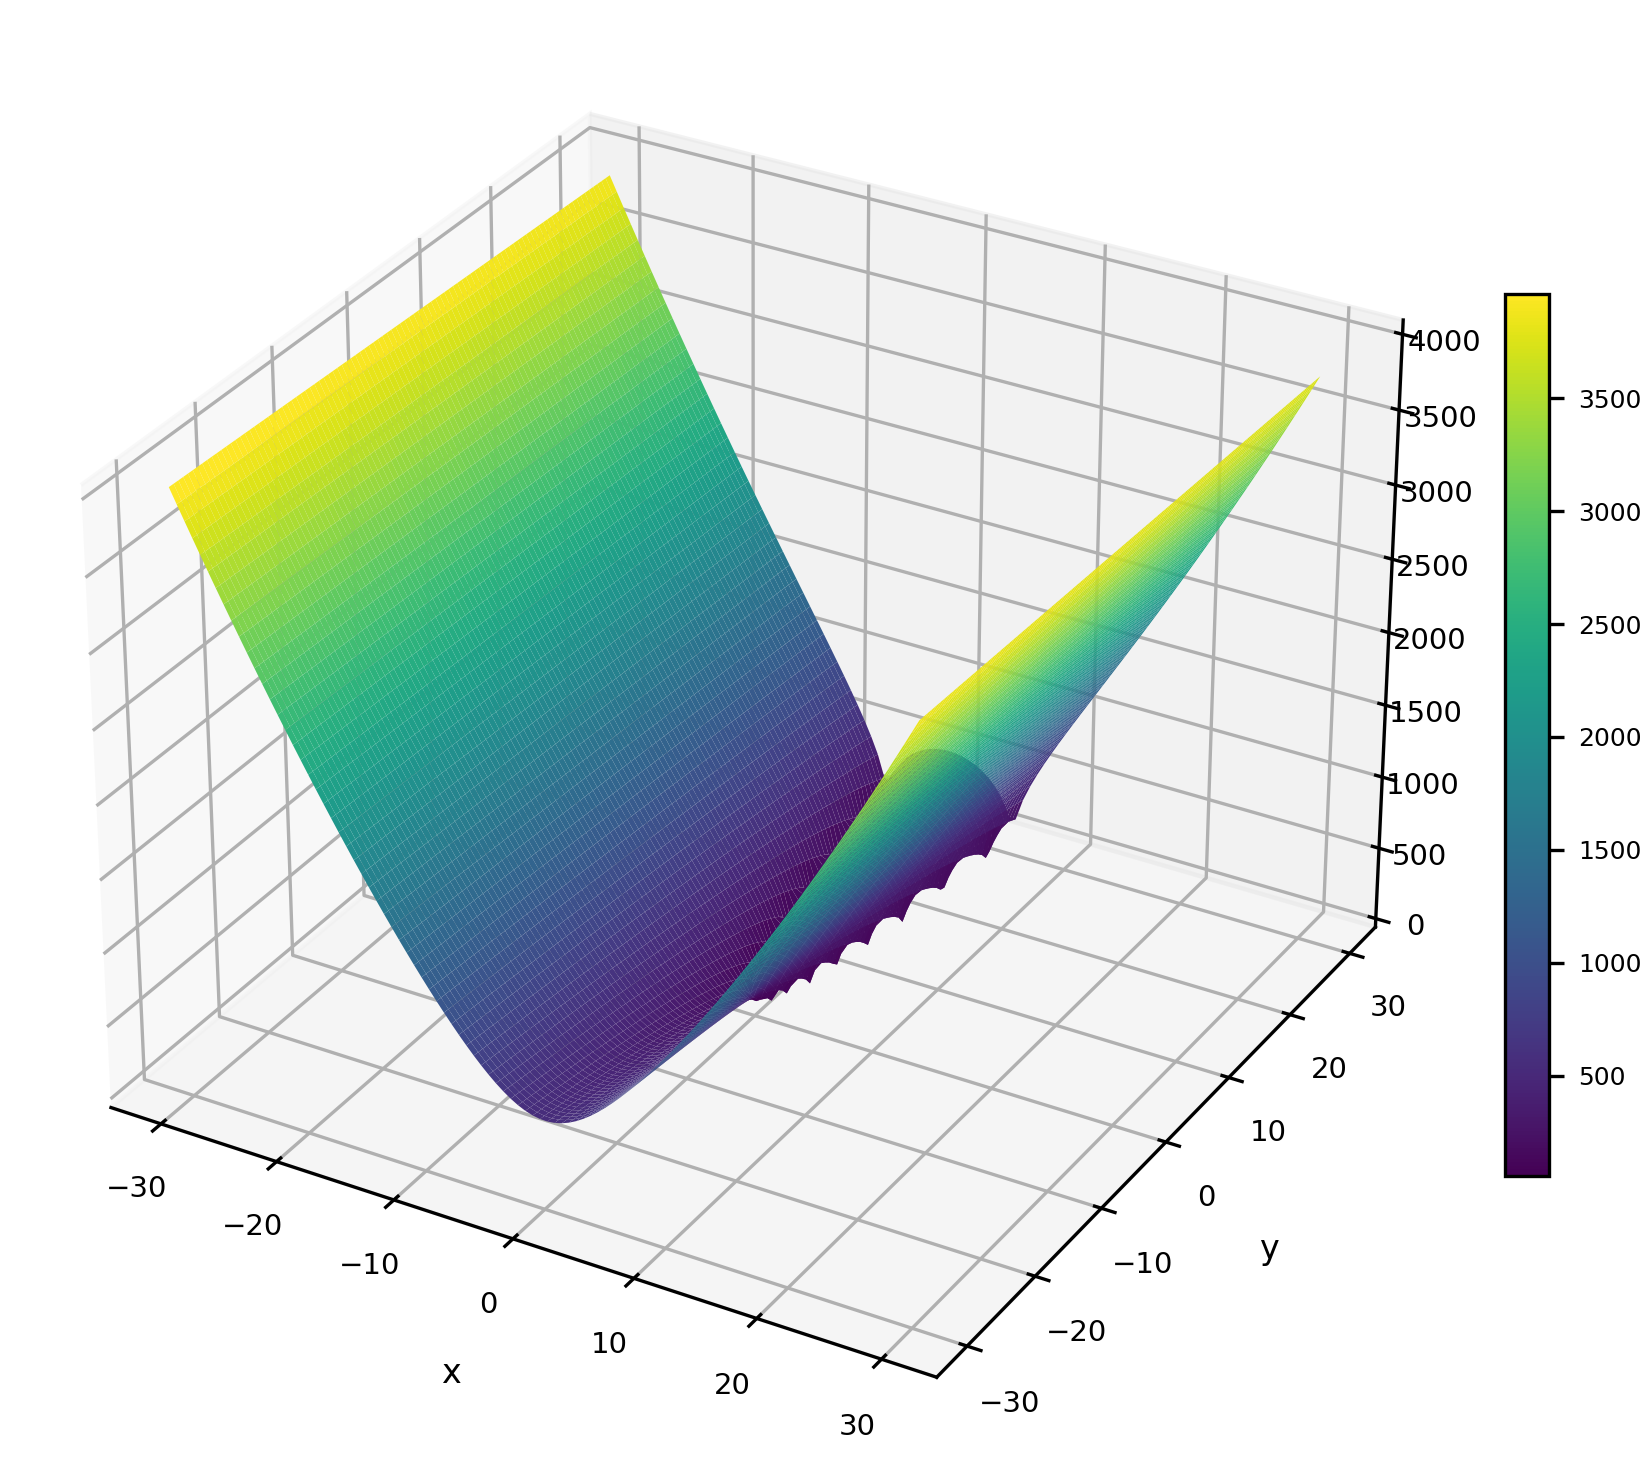
\includegraphics[width=1\textwidth]{Figures/benchmark_plots/Modified_Rosenbrock_No.02___Hollow_Ground_Bent_Knife_Edge_maximized.png}
        \caption{Modified Rosenbrock N.2}
    \end{subfigure}
    \begin{subfigure}{0.32\textwidth}
        \centering
        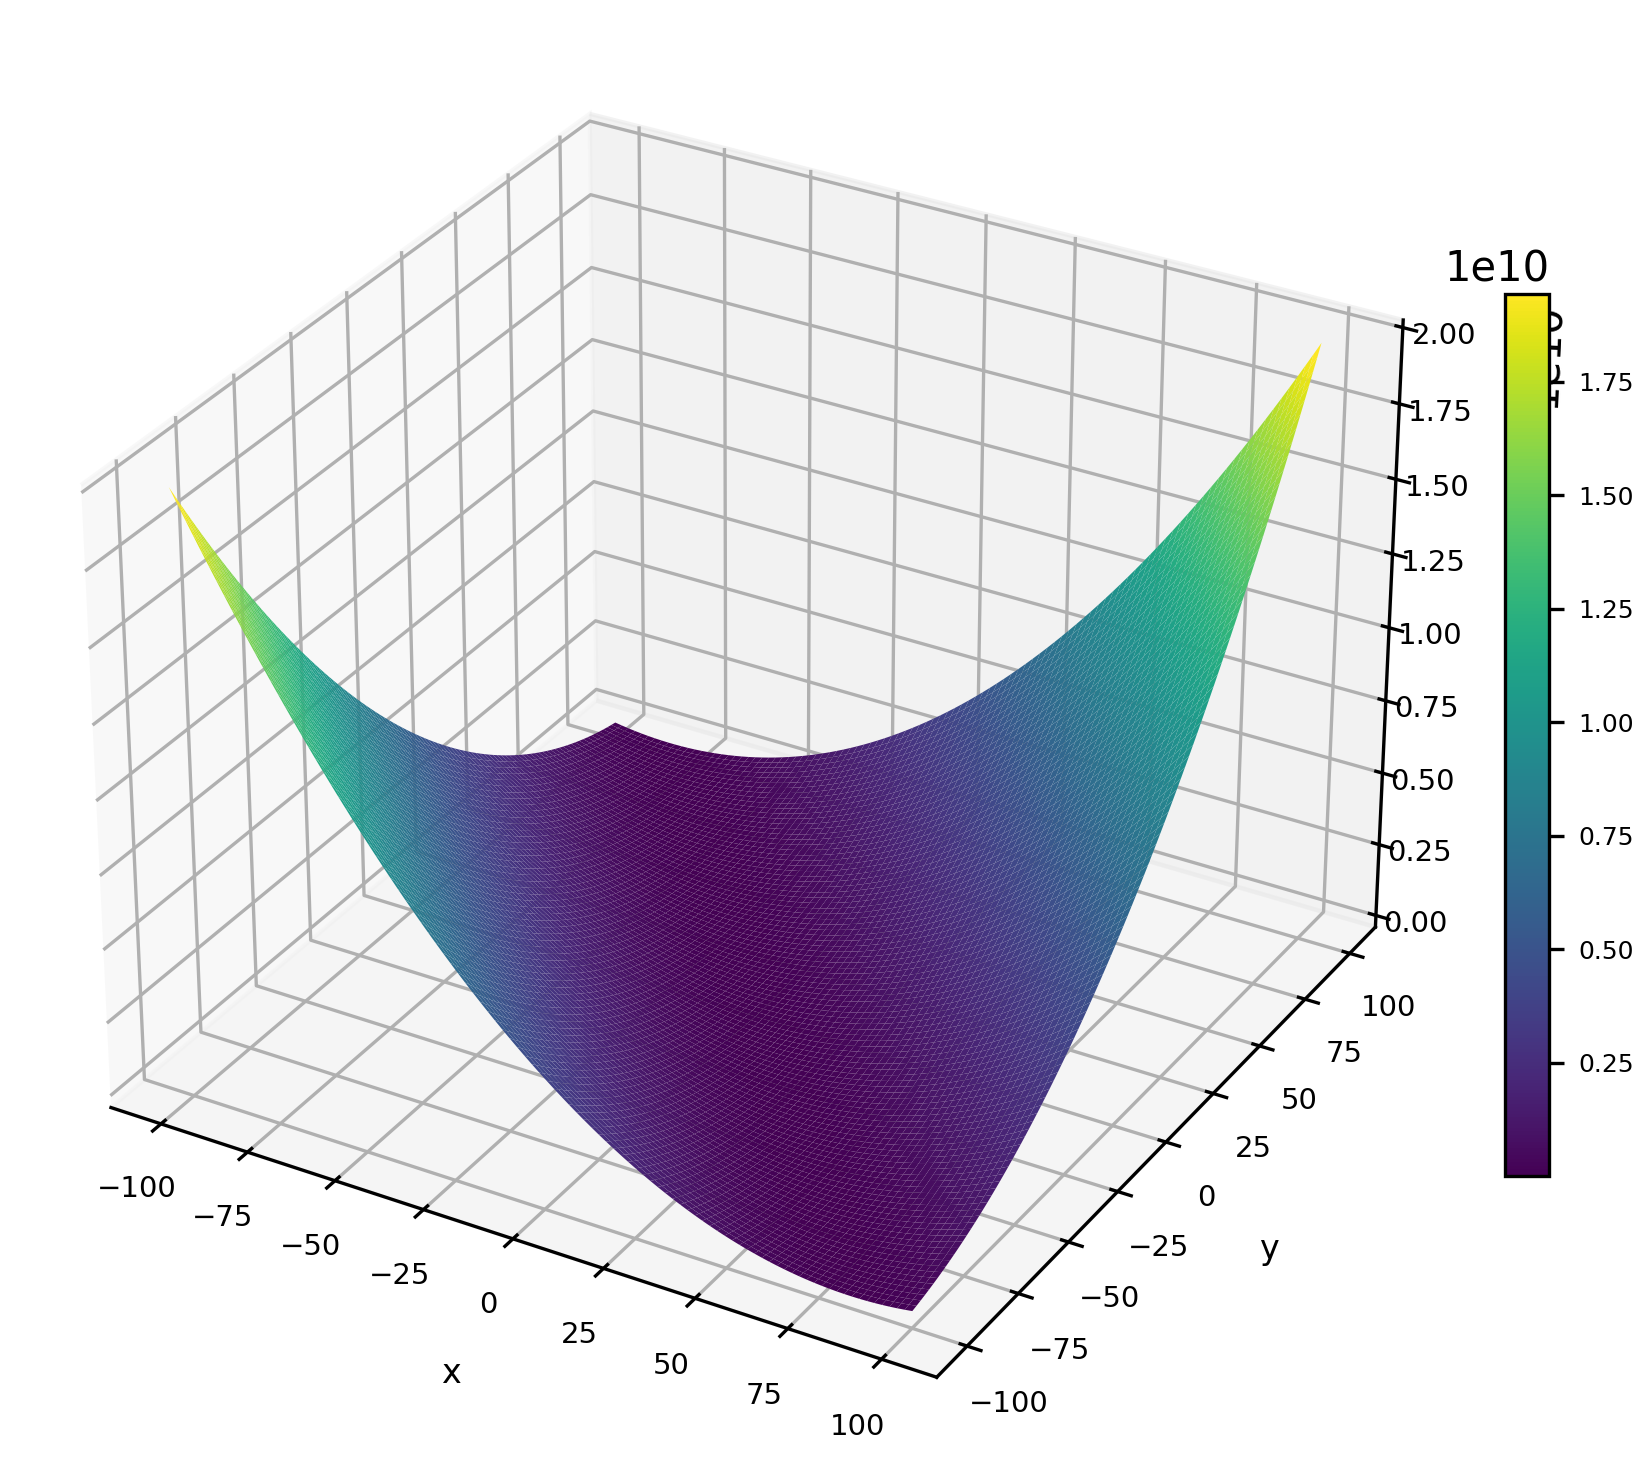
\includegraphics[width=1\textwidth]{Figures/benchmark_plots/Rotated_Bent_Cigar_maximized.png}
        \caption{Rotated Bent Cigar}
    \end{subfigure}
    % \hspace{.5cm} % Adjust the space as needed.
    \begin{subfigure}{0.32\textwidth}
        \centering
        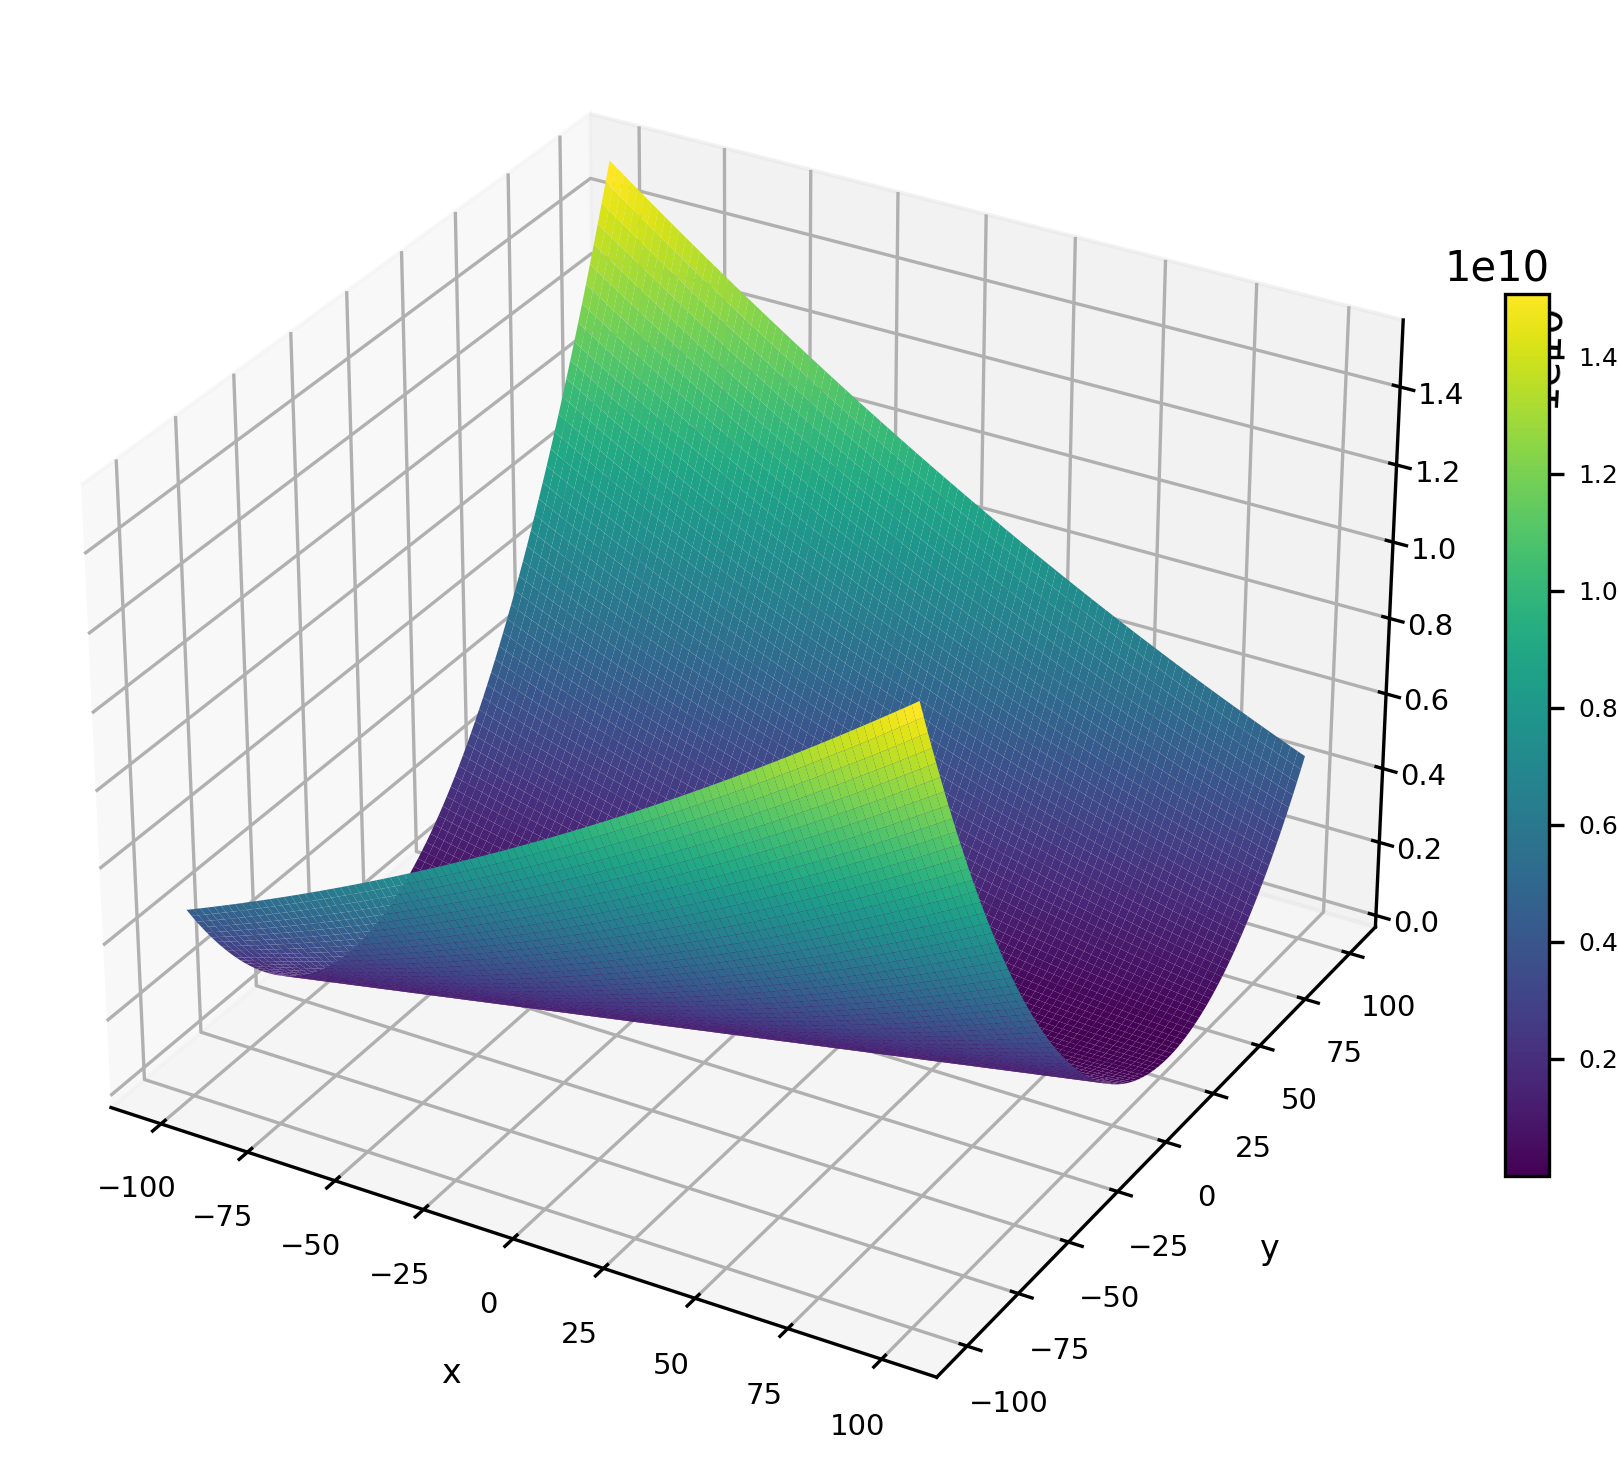
\includegraphics[width=1\textwidth]{Figures/benchmark_plots/Rotated_Discus_maximized.png}
        \caption{Rotated Bent Cigar}
    \end{subfigure}
        \begin{subfigure}{0.32\textwidth}
        \centering
        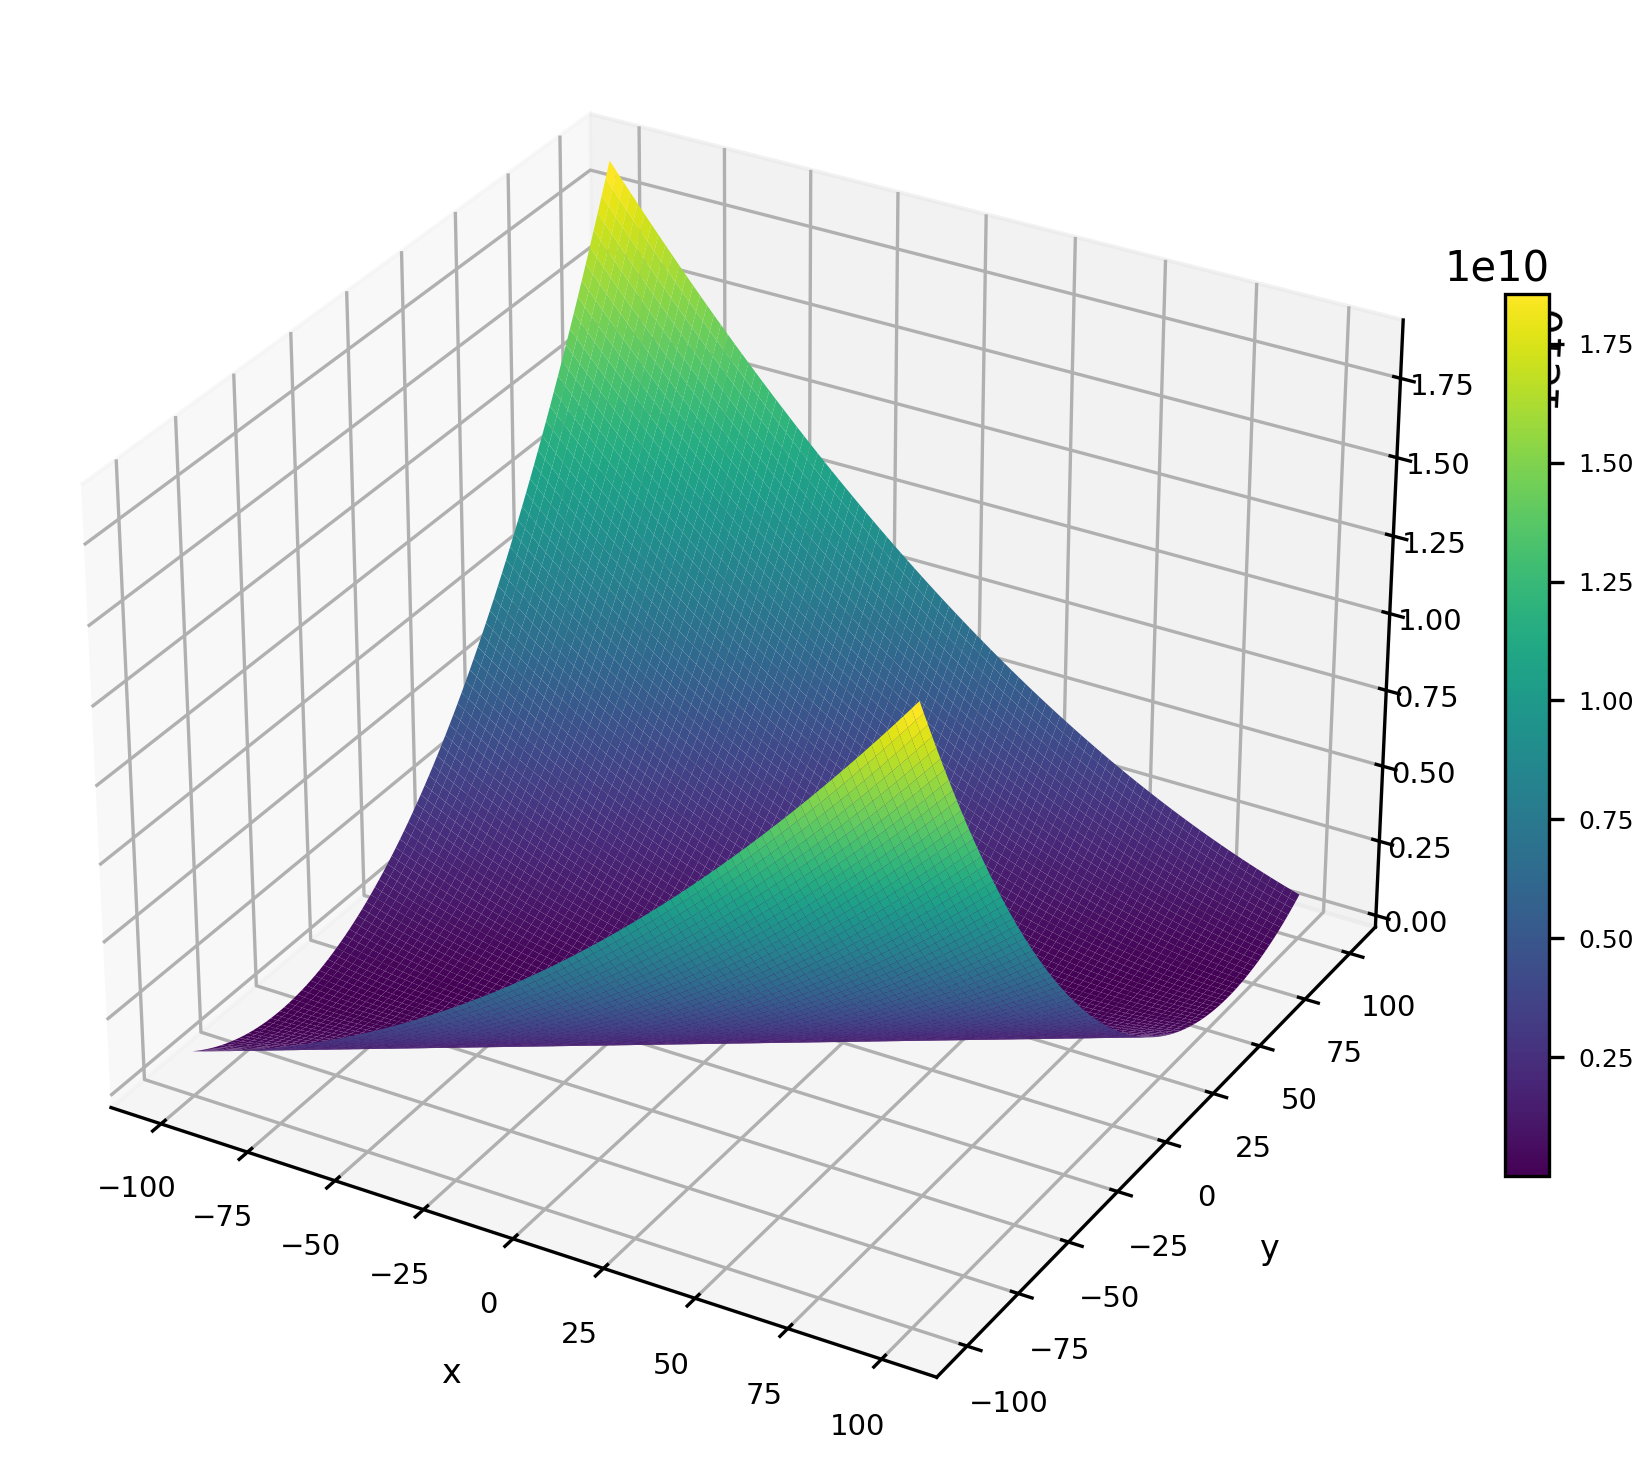
\includegraphics[width=1\textwidth]{Figures/benchmark_plots/Rotated_High_Conditioned_Elliptic_maximized.png}
        \caption{Rotated Discus}
    \end{subfigure}
    % \hspace{.5cm} % Adjust the space as needed.
    \begin{subfigure}{0.32\textwidth}
        \centering
        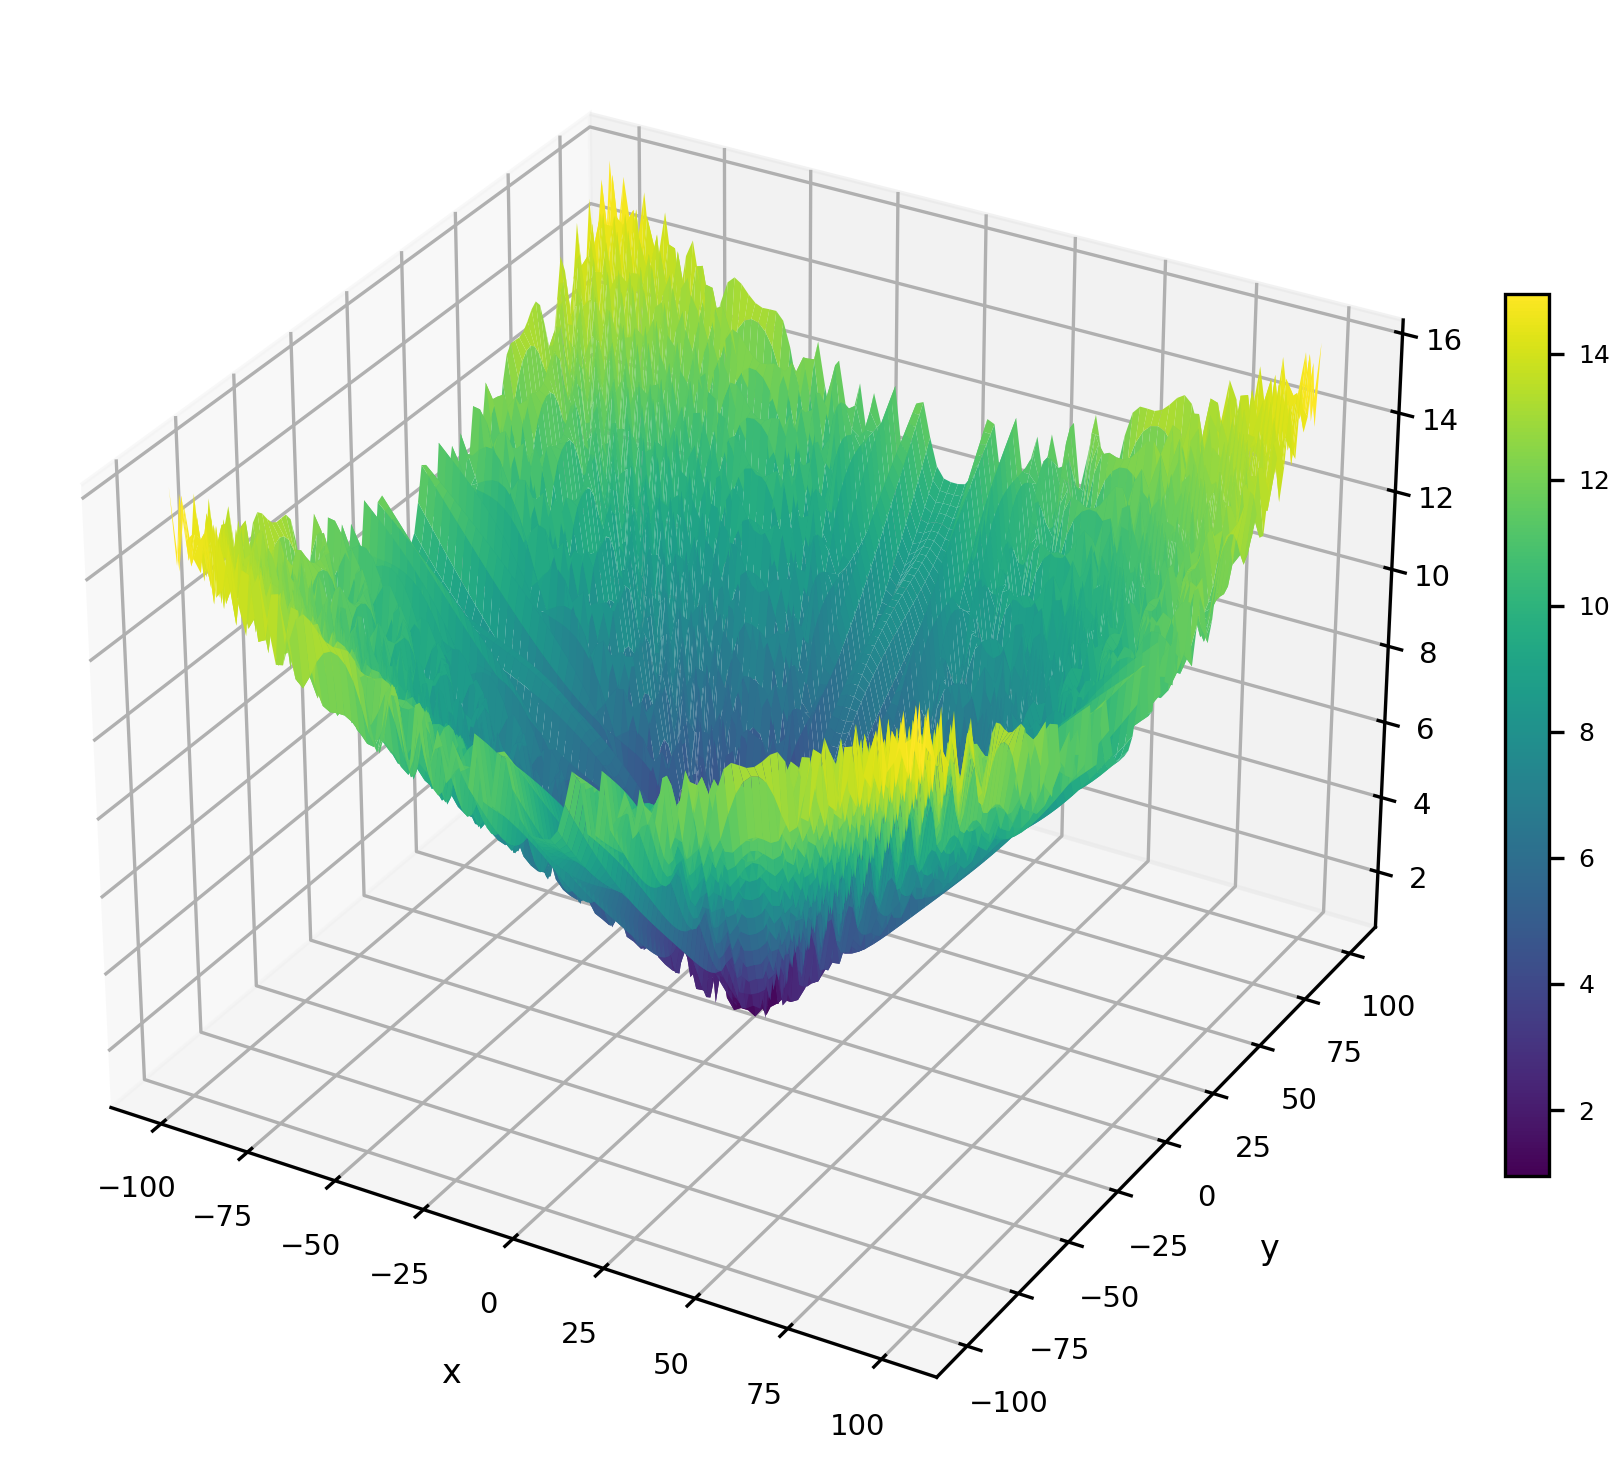
\includegraphics[width=1\textwidth]{Figures/benchmark_plots/Salomon_maximized.png}
        \caption{Salomon}
    \end{subfigure}
    \begin{subfigure}{0.32\textwidth}
        \centering
        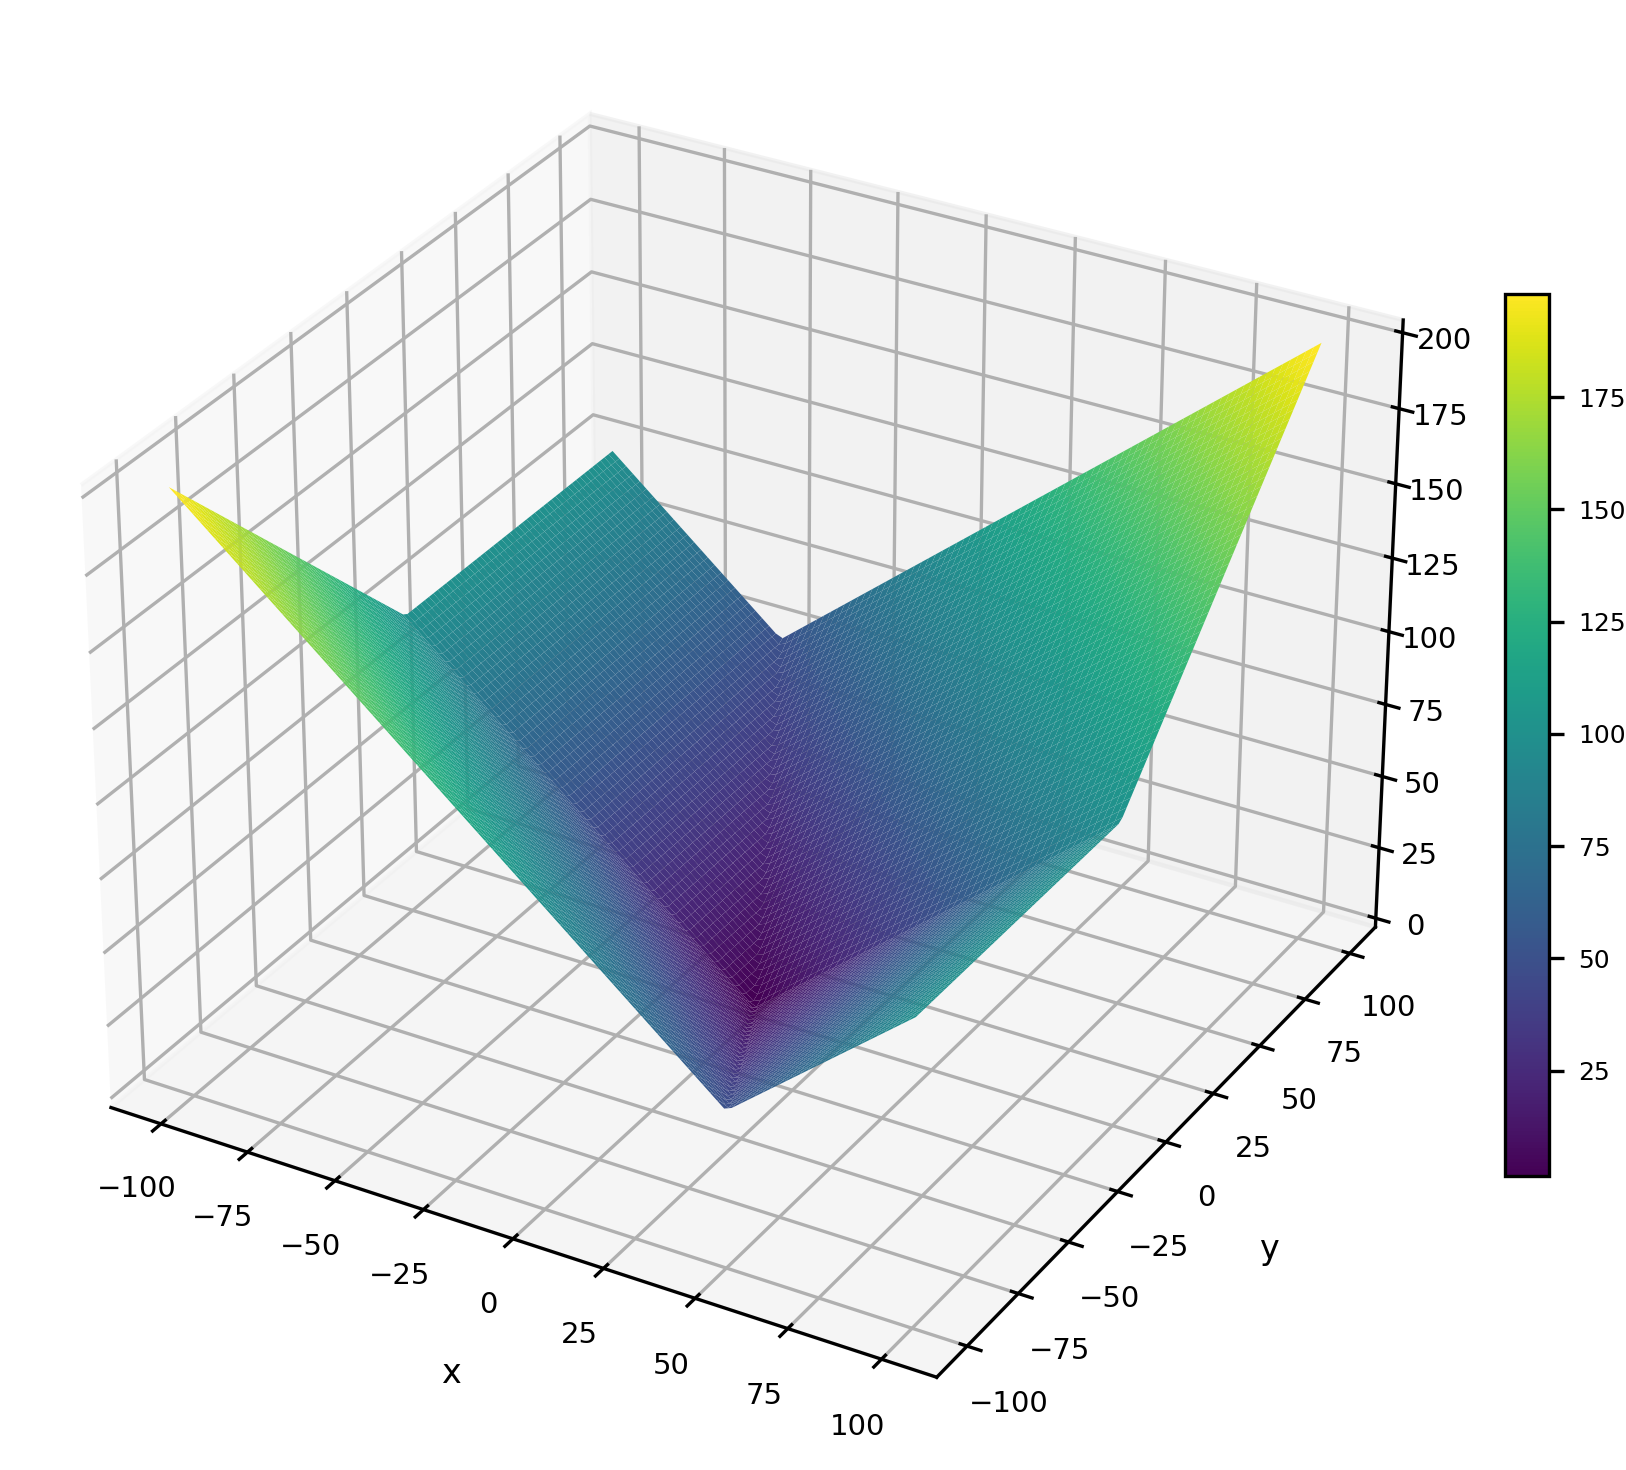
\includegraphics[width=1\textwidth]{Figures/benchmark_plots/Schwefel_N20_maximized.png}
        \caption{Schwefel N.2.0}
    \end{subfigure}
    % \hspace{.5cm} % Adjust the space as needed.
    \begin{subfigure}{0.32\textwidth}
        \centering
        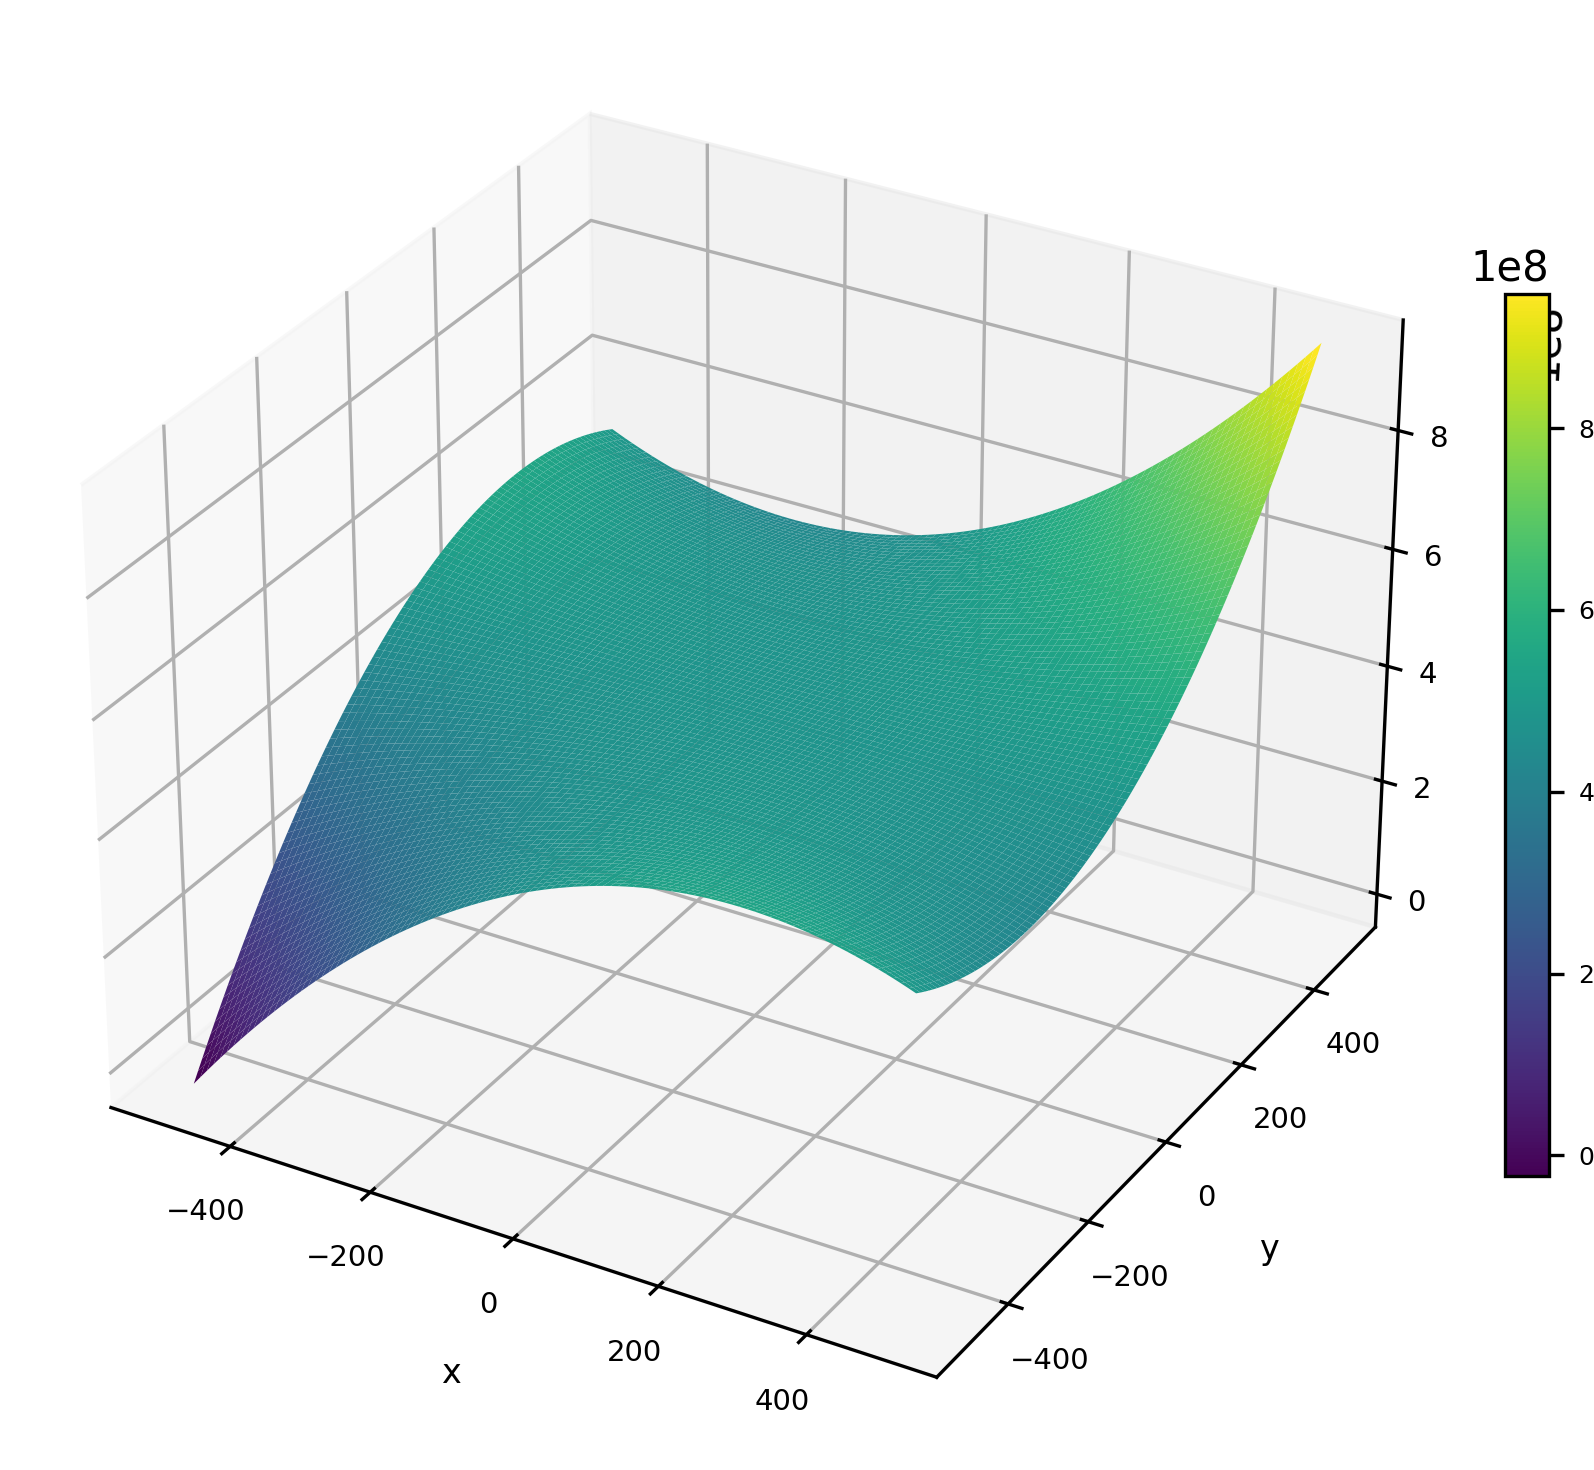
\includegraphics[width=1\textwidth]{Figures/benchmark_plots/Schwefel_N36_maximized.png}
        \caption{Schwefel N.3.6}
    \end{subfigure}
        \captionsetup{list=no}
\caption{Two-dimensional visualizations of benchmark problem landscapes.}
\end{figure}

\begin{figure}[p]\ContinuedFloat
\renewcommand\thesubfigure{A.\arabic{subfigure}} % Local change starts here
    \centering
    \begin{subfigure}{0.32\textwidth}
        \centering
        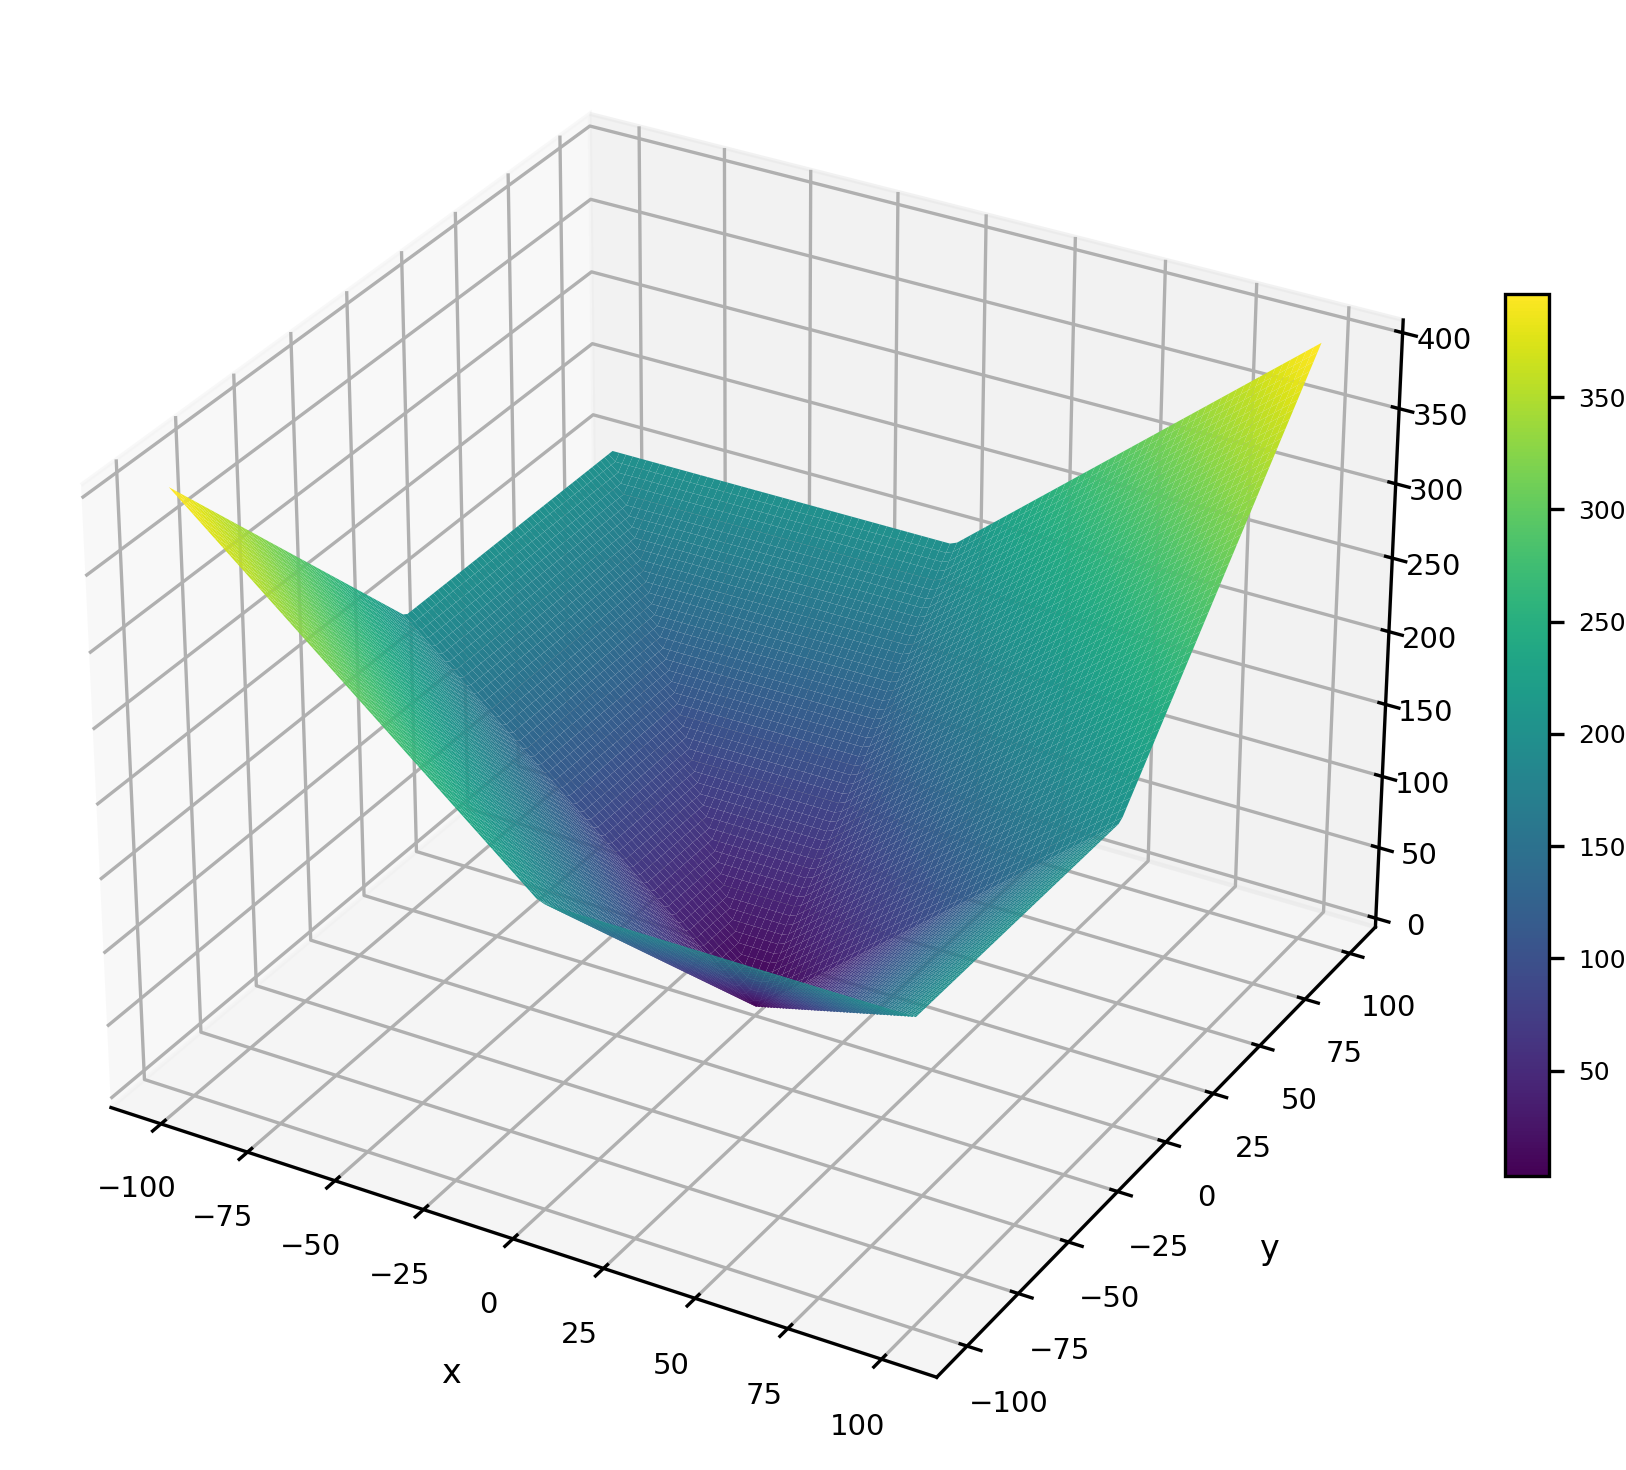
\includegraphics[width=1\textwidth]{Figures/benchmark_plots/Schwefel_N6_maximized.png}
        \caption{Schwefel N.6}
    \end{subfigure}
    % \hspace{.5cm} % Adjust the space as needed.
    \begin{subfigure}{0.32\textwidth}
        \centering
        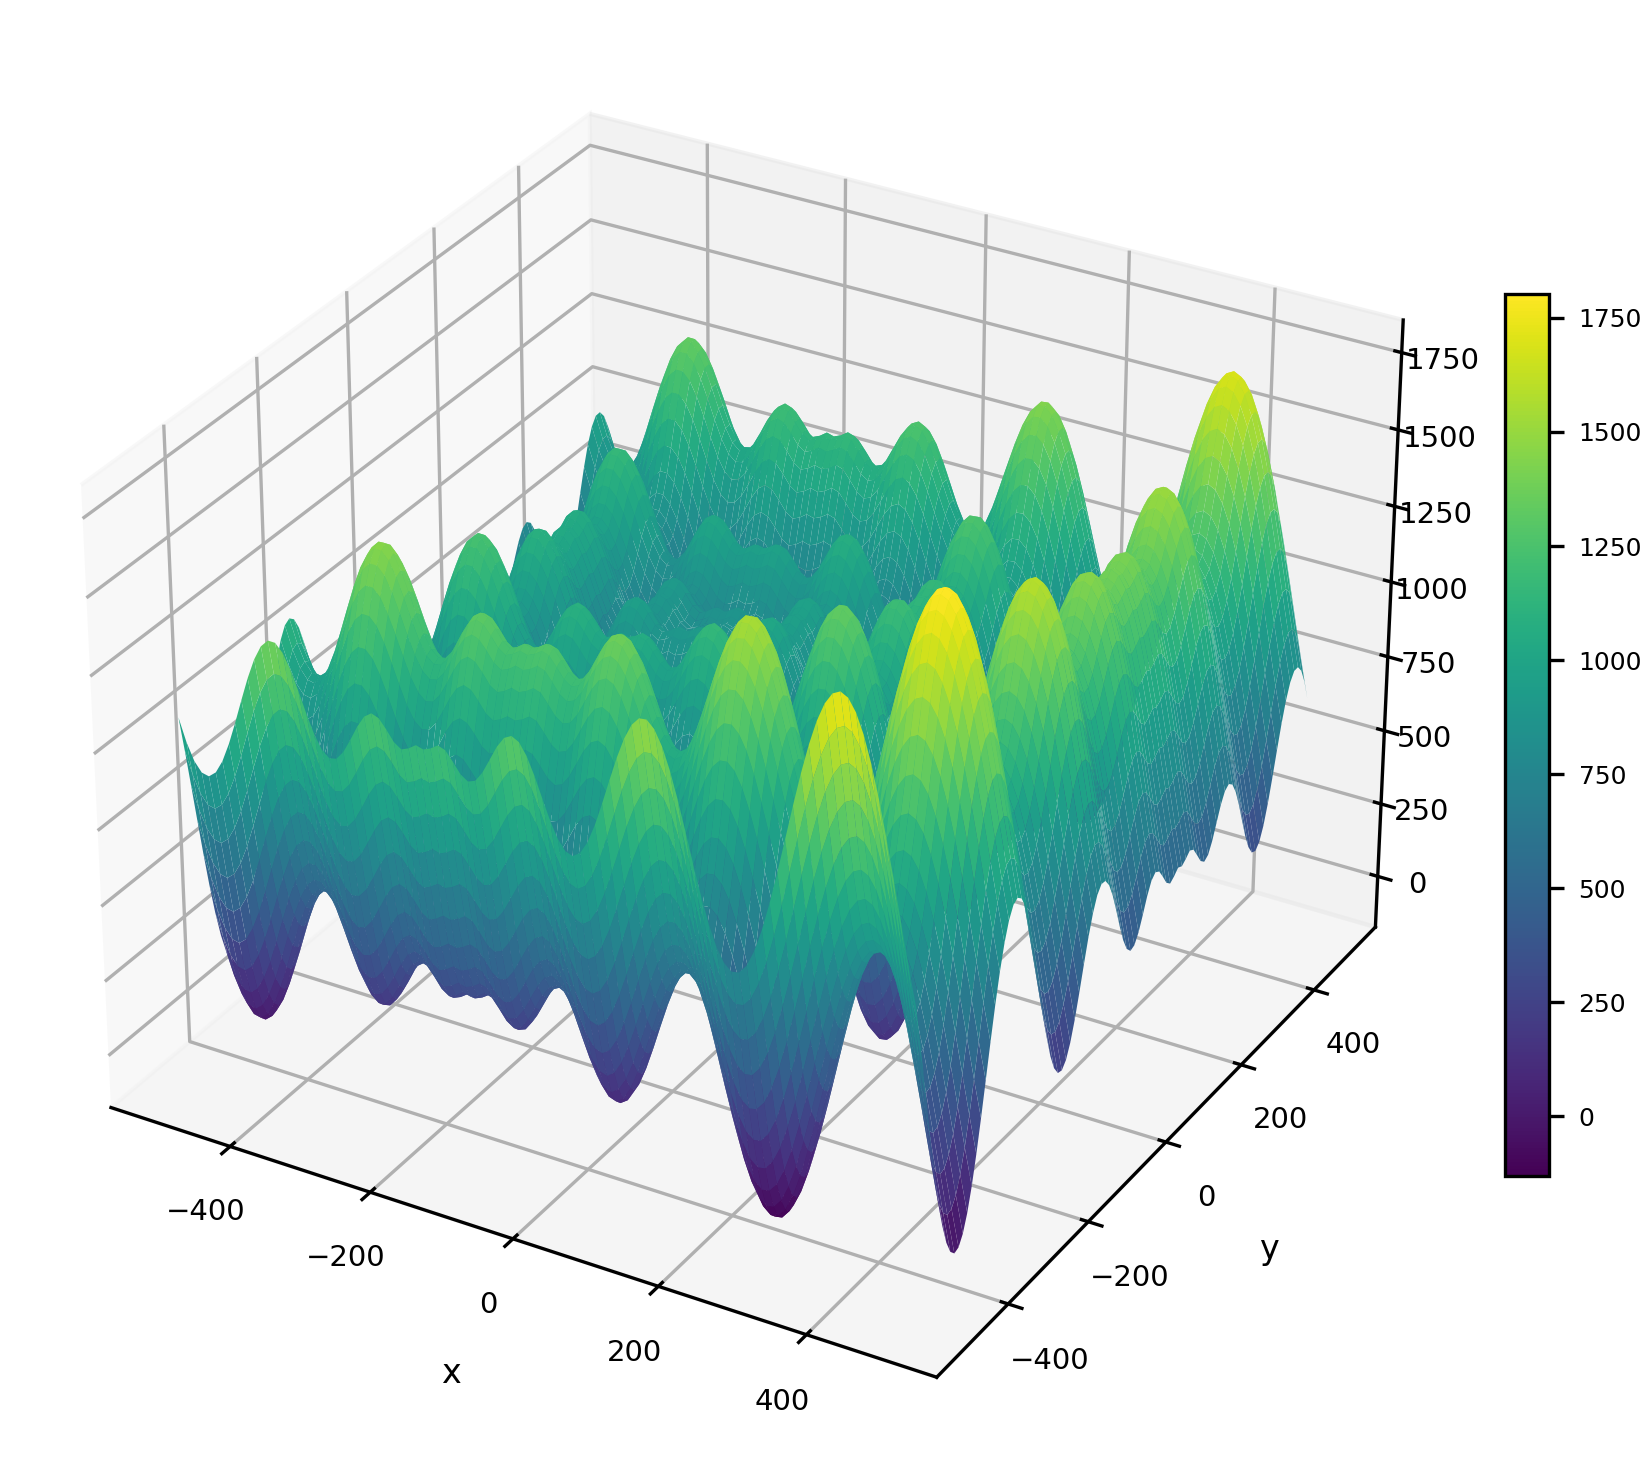
\includegraphics[width=1\textwidth]{Figures/benchmark_plots/Shifted_Schwefel_maximized.png}
        \caption{Shifted Schwefel (N.2.6)}
    \end{subfigure}
    \begin{subfigure}{0.32\textwidth}
        \centering
        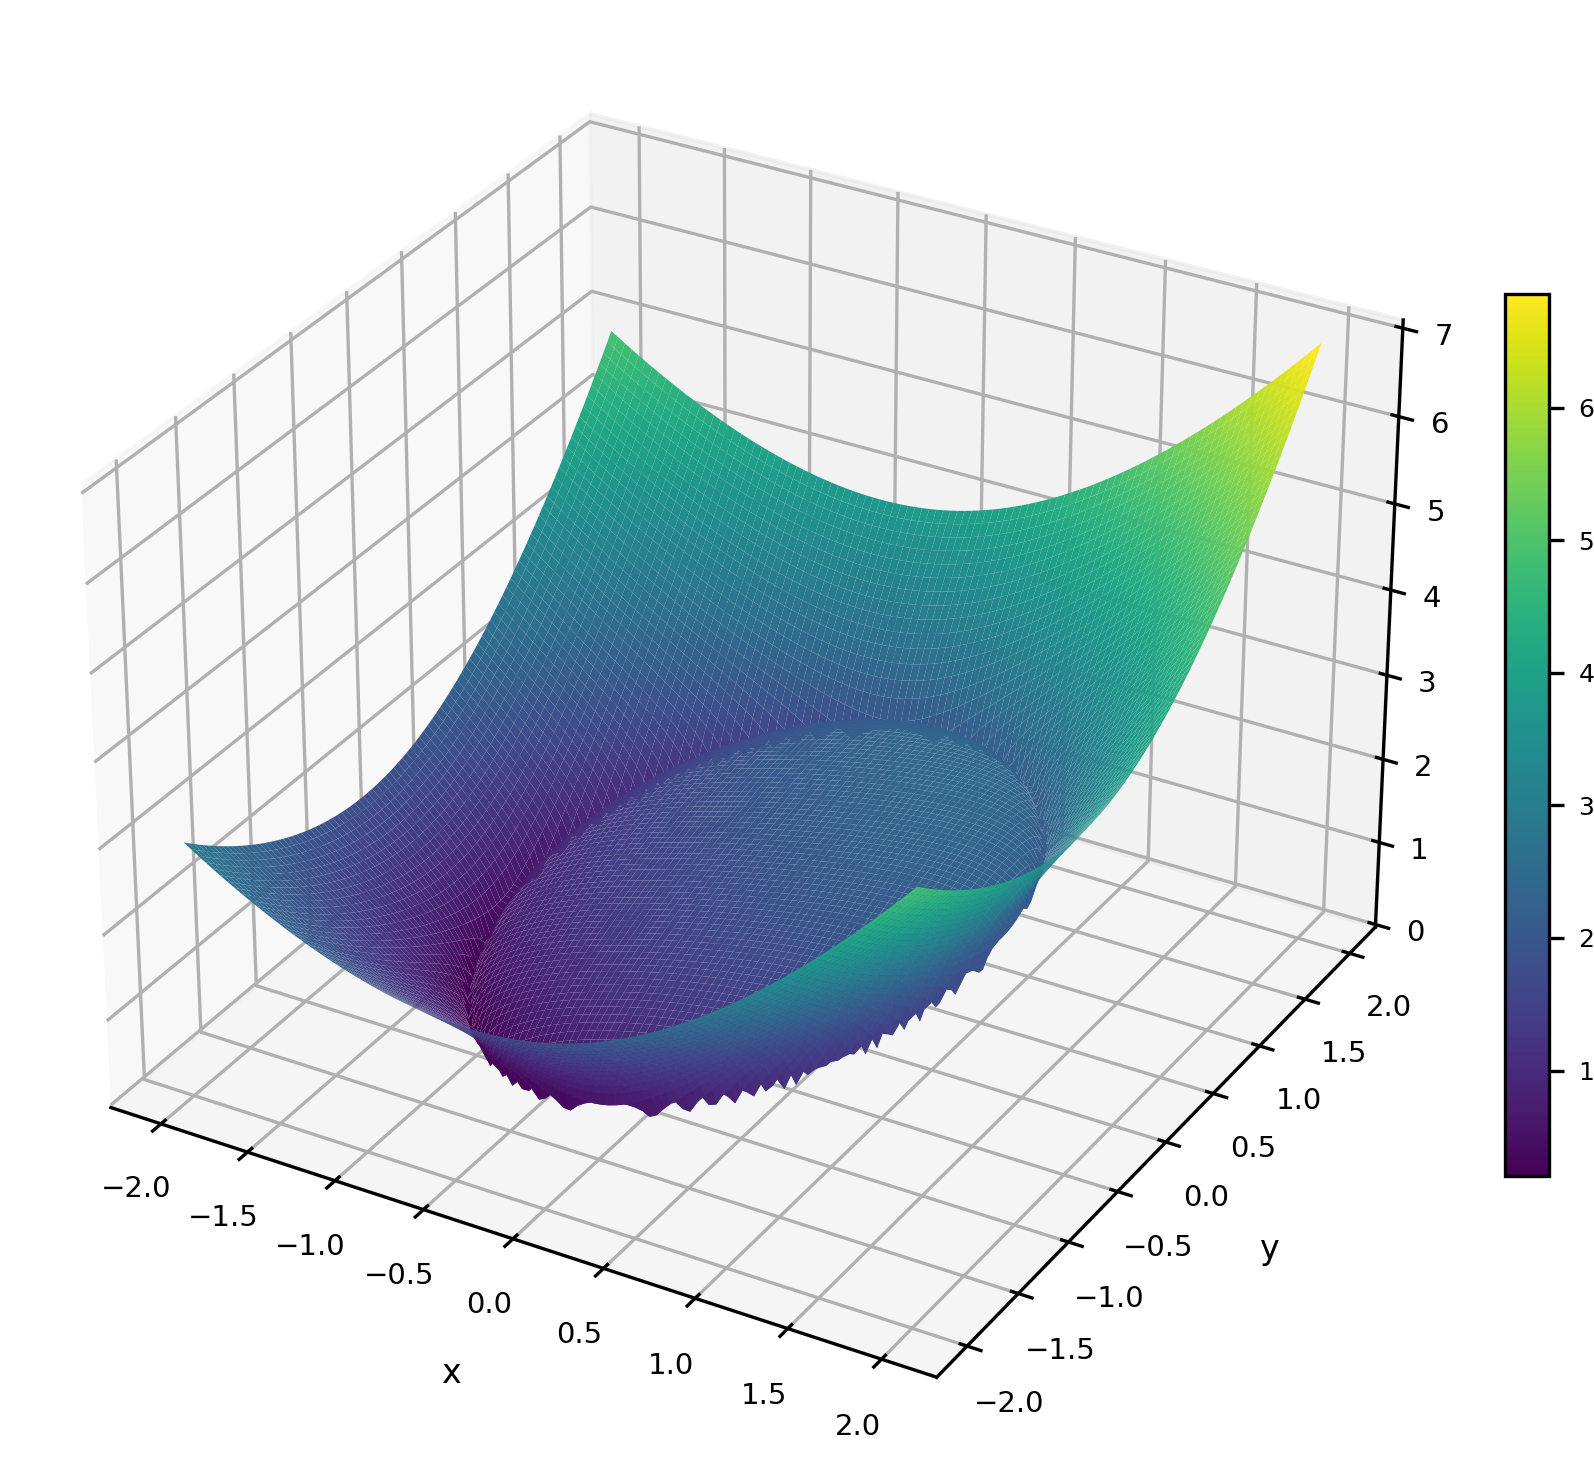
\includegraphics[width=1\textwidth]{Figures/benchmark_plots/Happy_Cat_maximized.png}
        \caption{HappyCat}
    \end{subfigure}
    % % \hspace{.5cm} % Adjust the space as needed.
    \begin{subfigure}{0.32\textwidth}
        \centering
        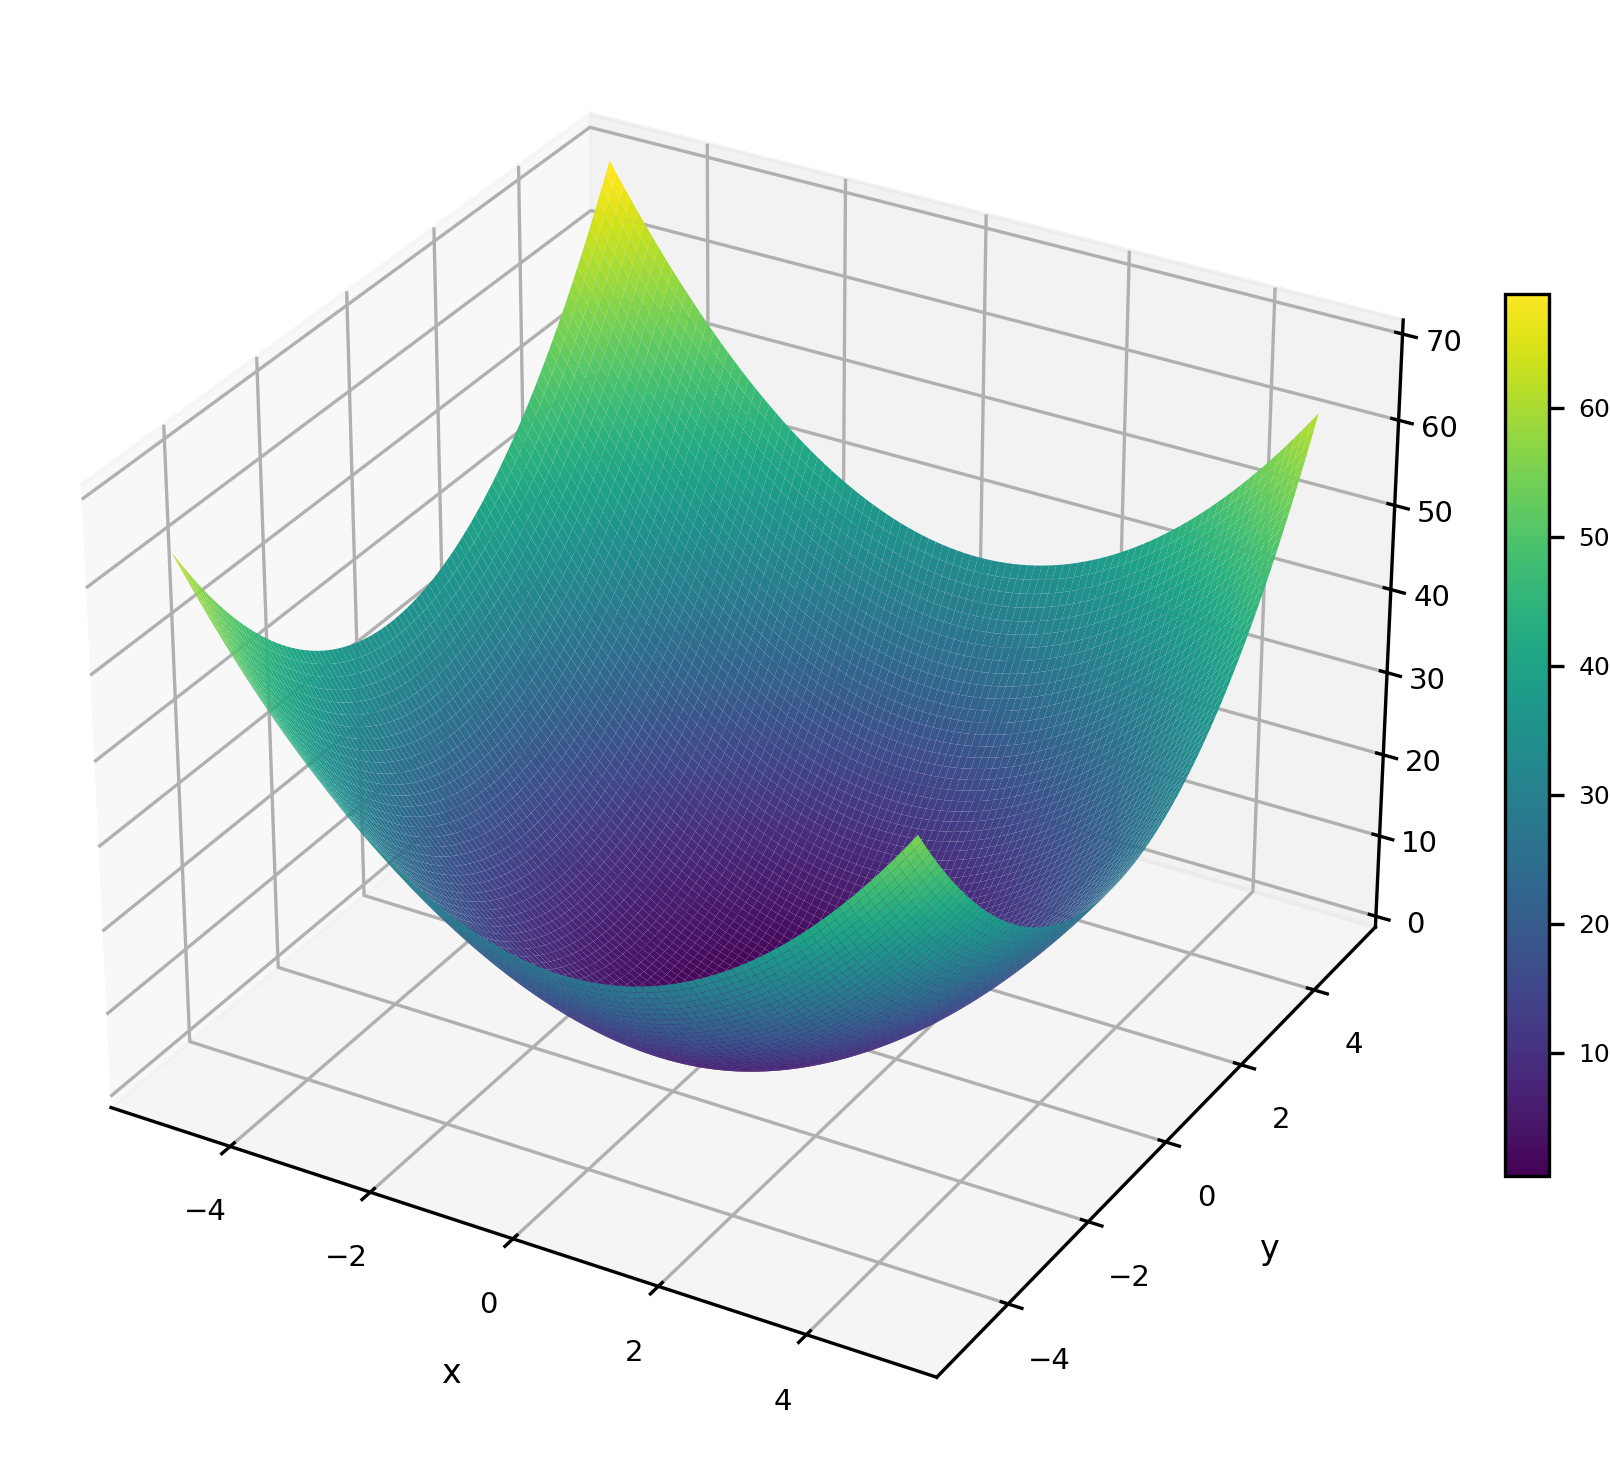
\includegraphics[width=1\textwidth]{Figures/benchmark_plots/Shifted_and_Rotated_HGBat_maximized.png}
        \caption{HGBat}
    \end{subfigure}
        \begin{subfigure}{0.32\textwidth}
        \centering
        \includegraphics[width=1\textwidth]{Figures/benchmark_plots/Shifted_and_Rotated_Expanded_Scaffer’s_F6_maximized.png}
        \caption{Schaffer F7}
    \end{subfigure}
        \begin{subfigure}{0.32\textwidth}
        \centering
        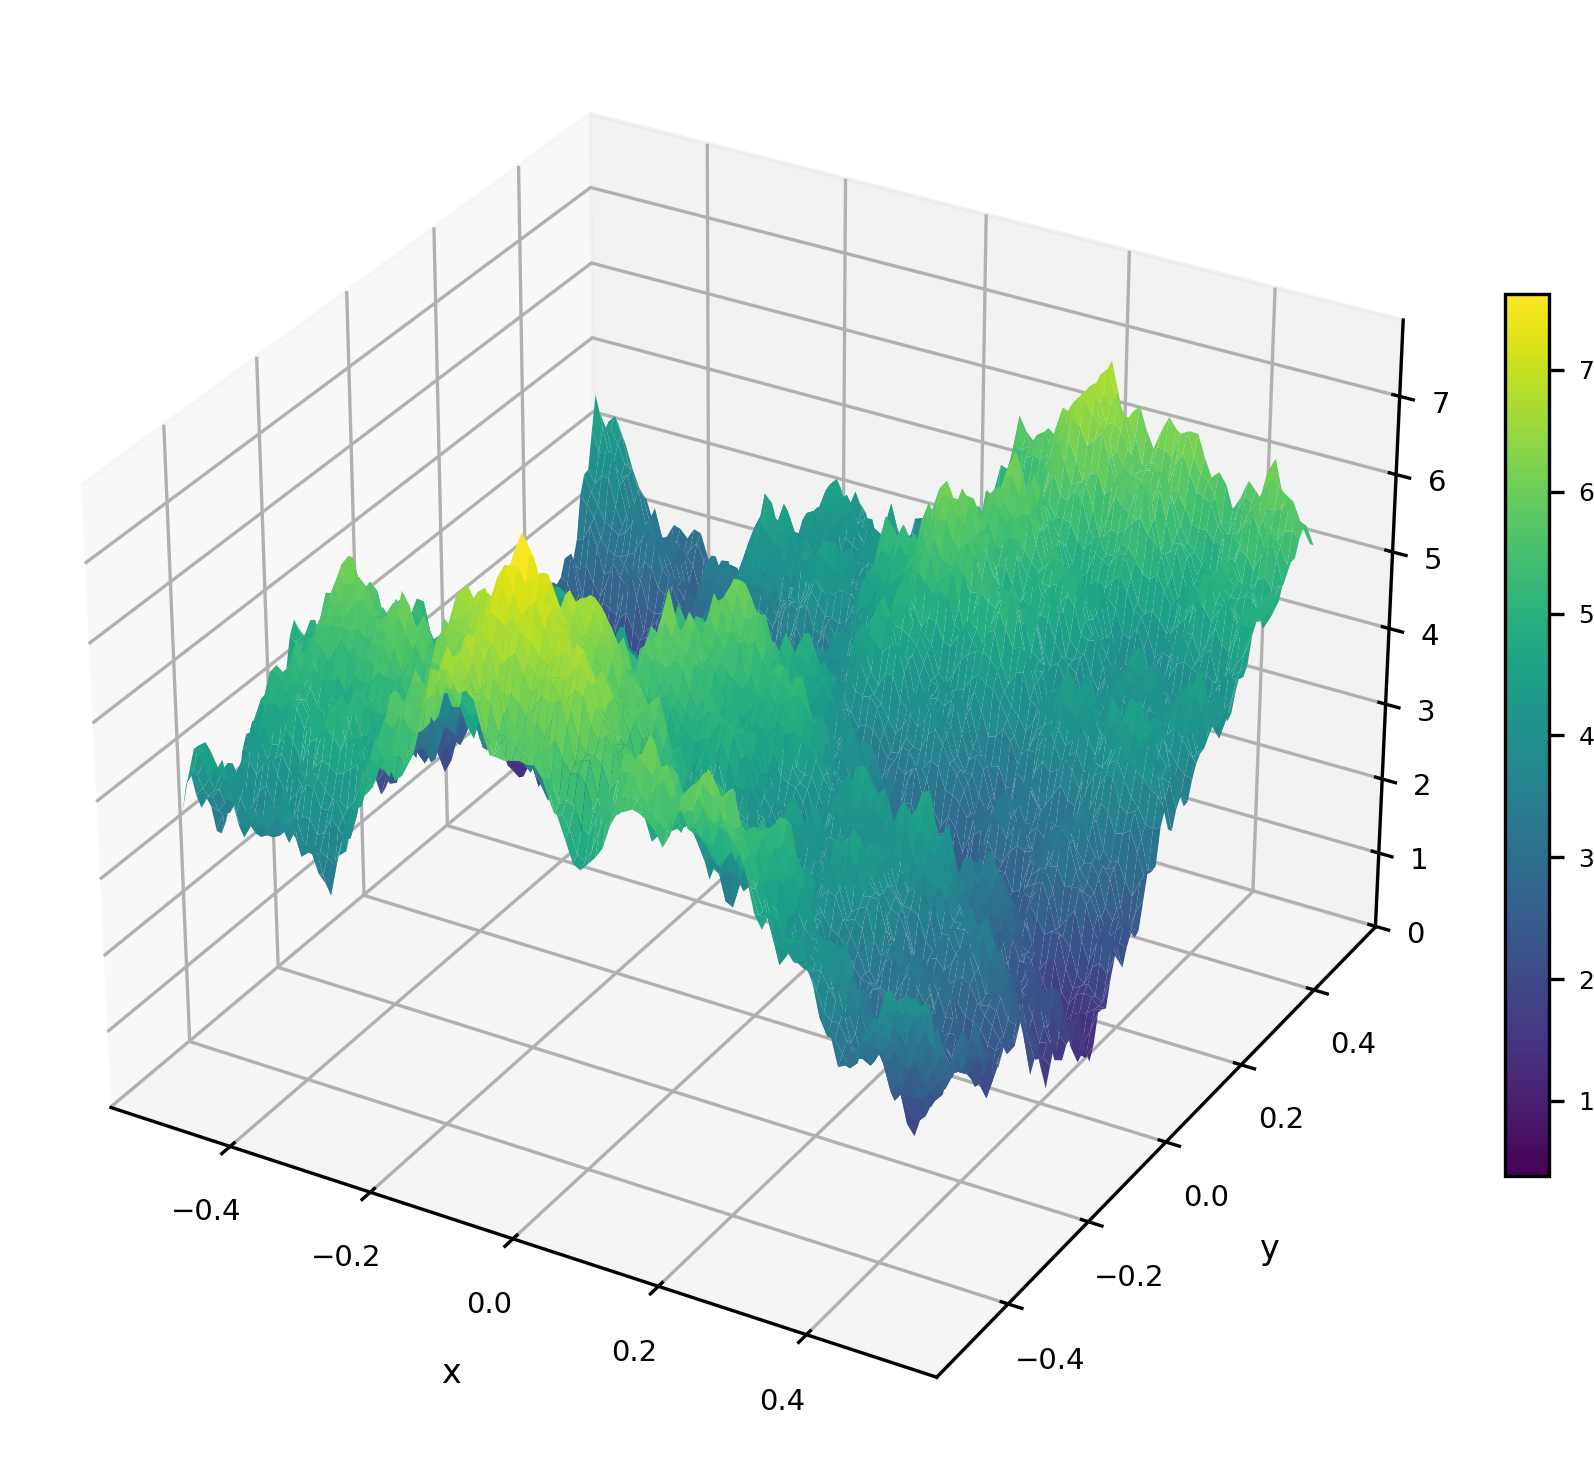
\includegraphics[width=1\textwidth]{Figures/benchmark_plots/Shifted_and_Rotated_Weierstrass_maximized.png}
        \caption{Weierstrass}
    \end{subfigure}
    % \hspace{.5cm} % Adjust the space as needed.
    \begin{subfigure}{0.32\textwidth}
        \centering
        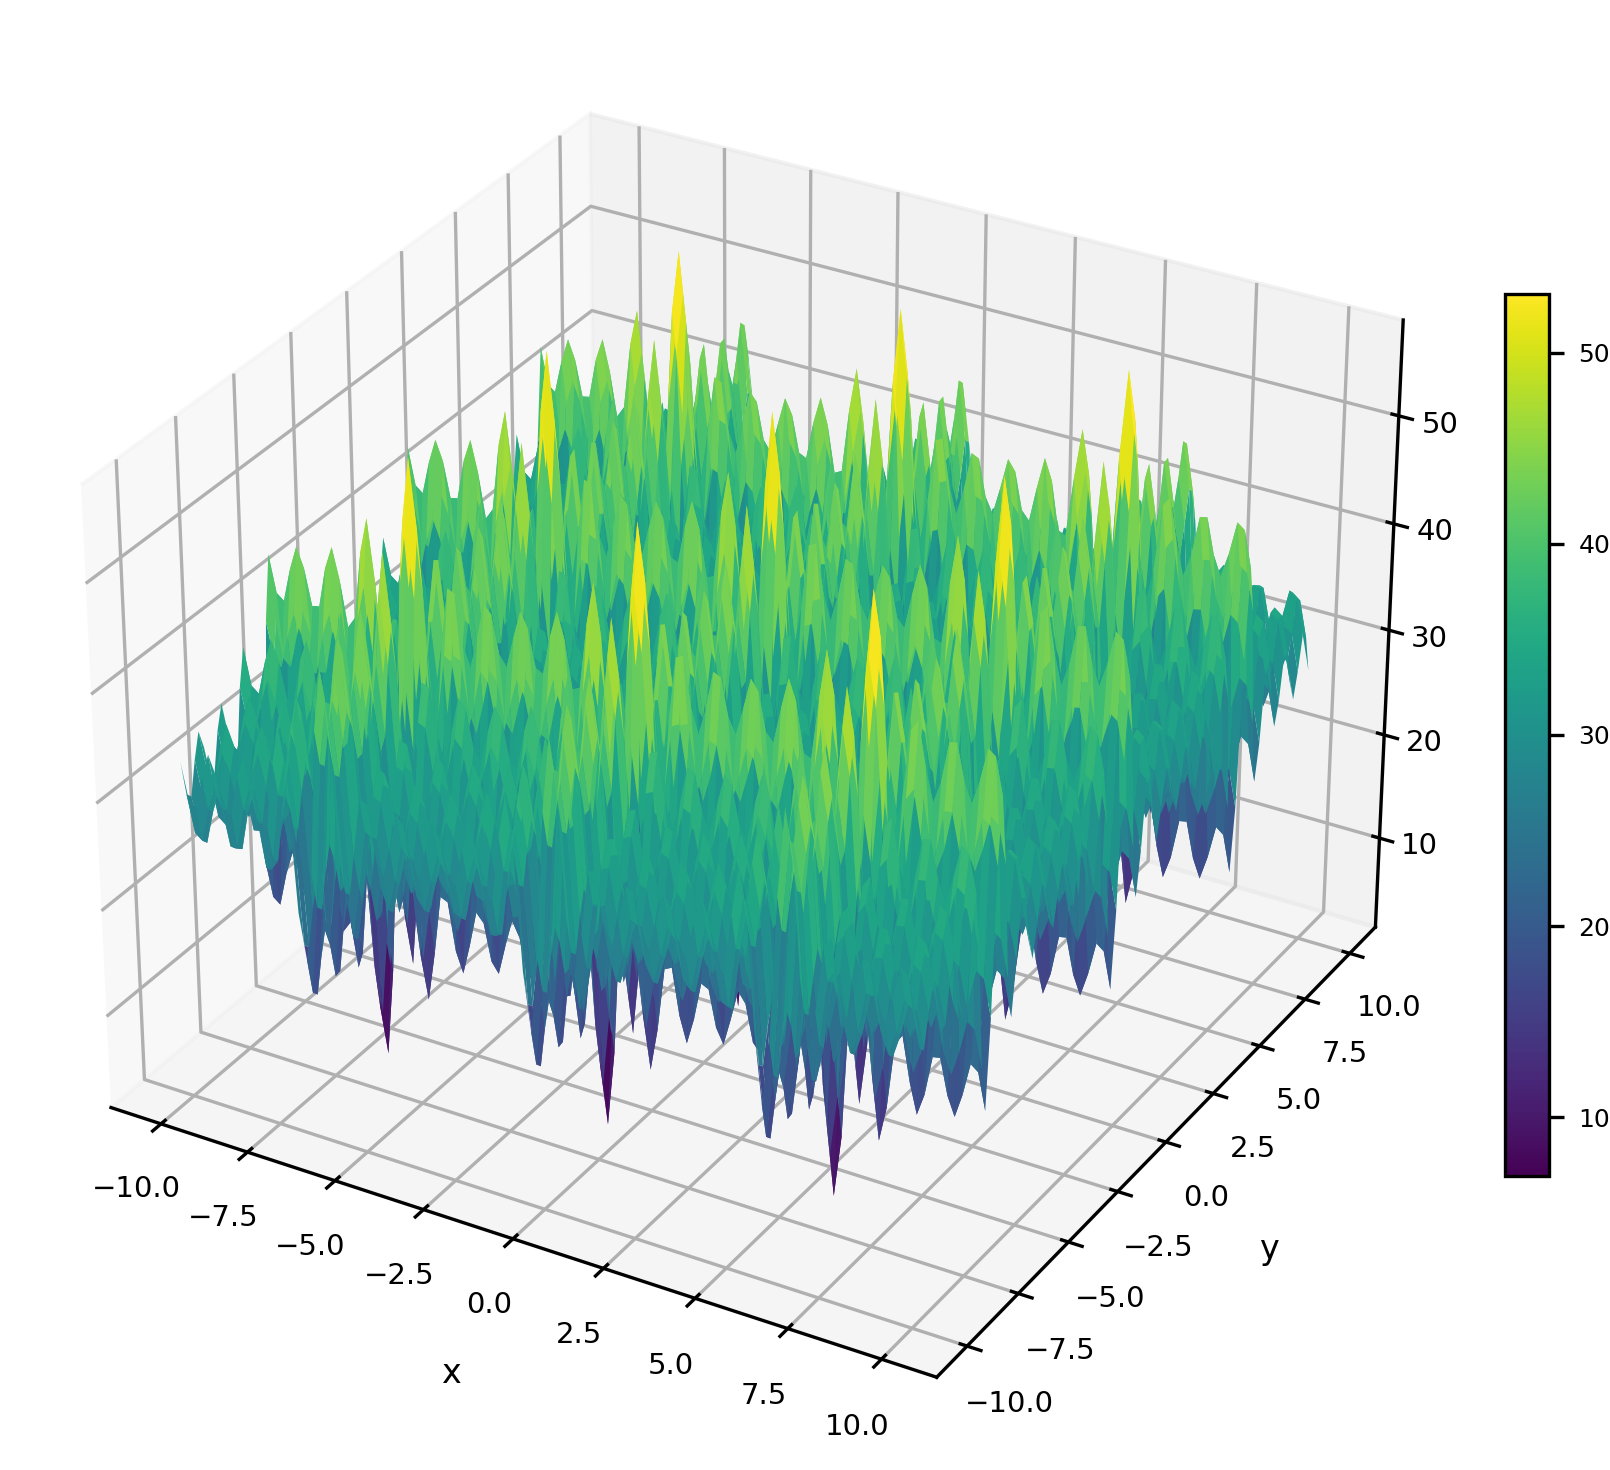
\includegraphics[width=1\textwidth]{Figures/benchmark_plots/Shubert_N3_maximized.png}
        \caption{Shubert N.3}
    \end{subfigure}
    % \hspace{.5cm} % Adjust the space as needed.
    \begin{subfigure}{0.32\textwidth}
        \centering
        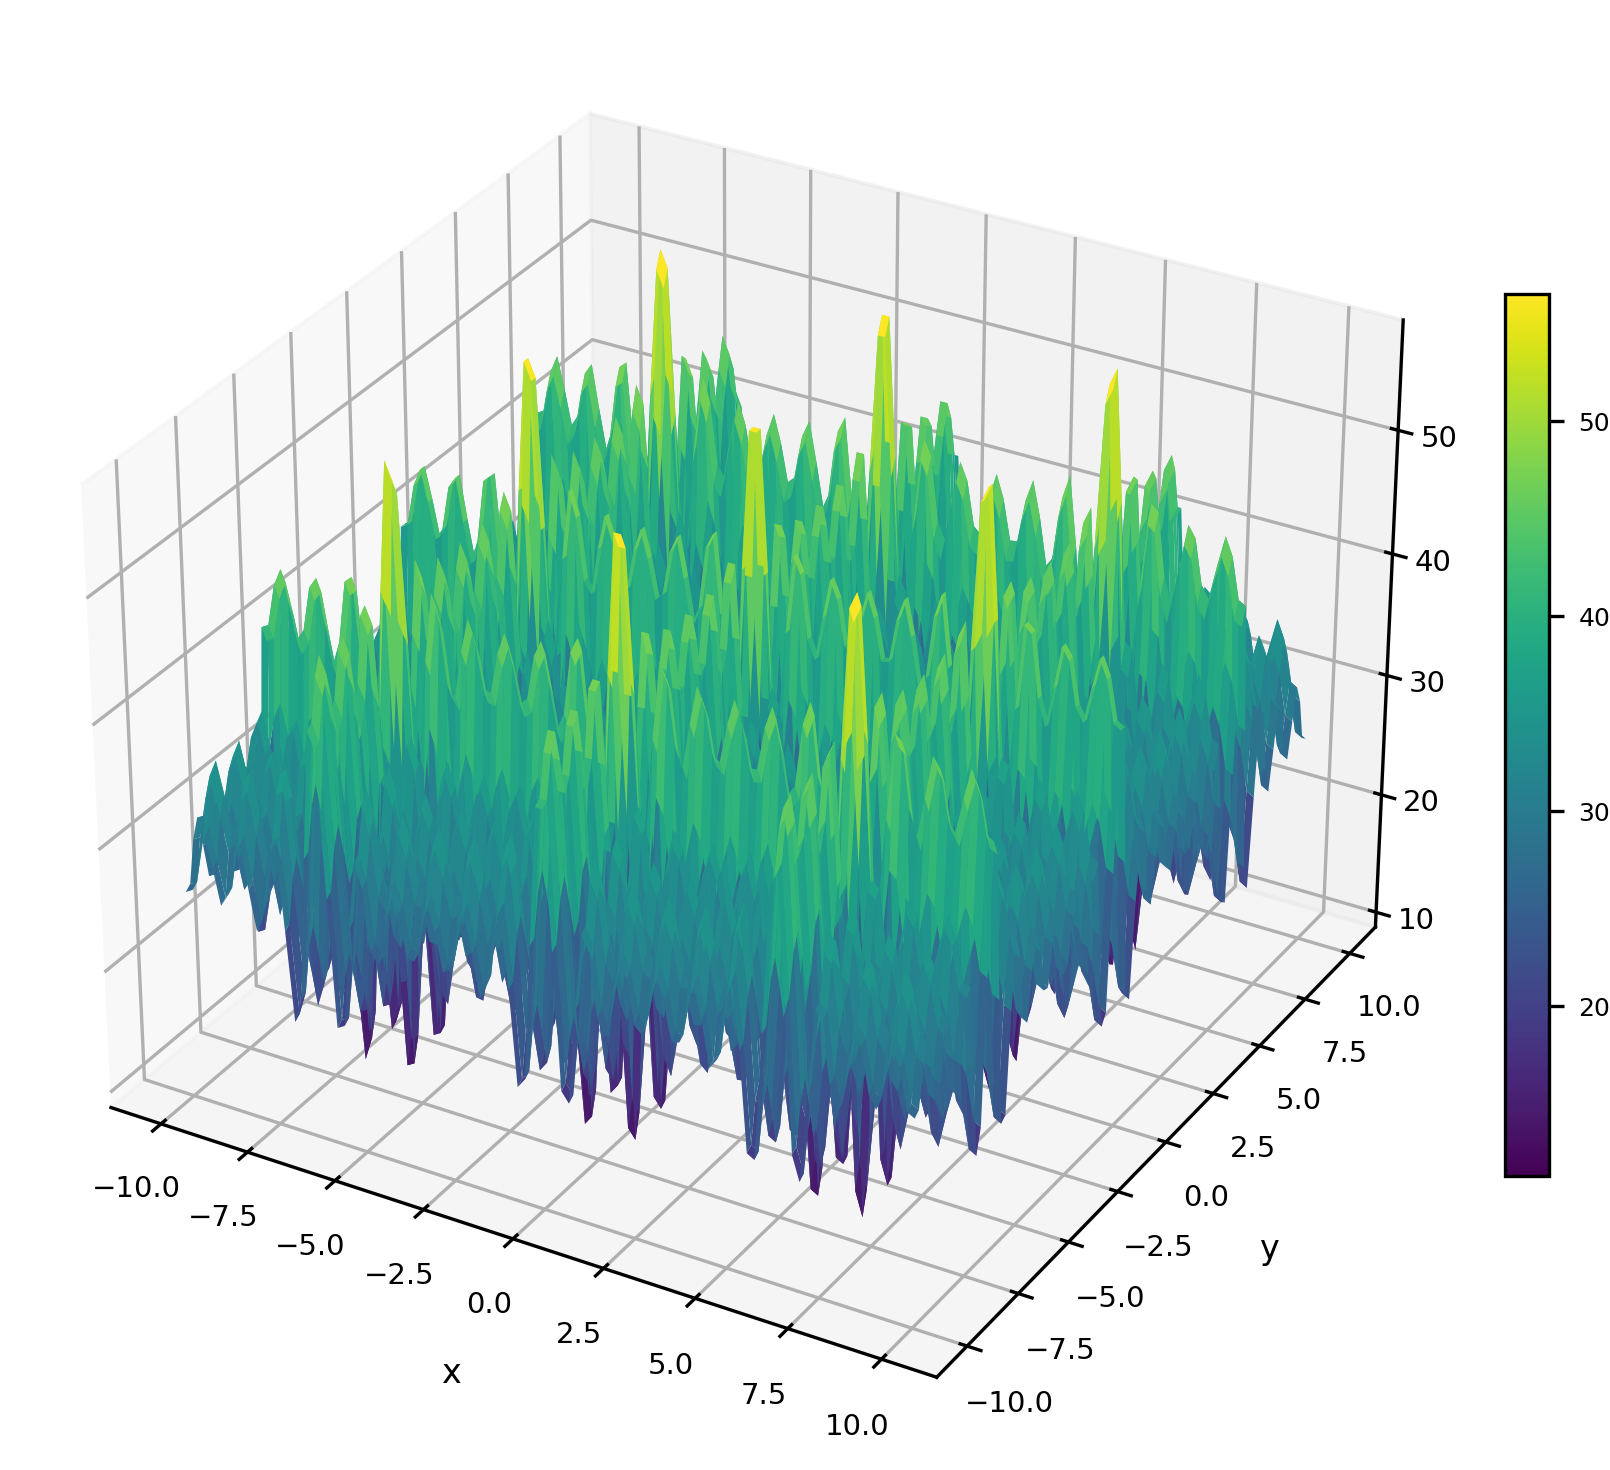
\includegraphics[width=1\textwidth]{Figures/benchmark_plots/Shubert_N4_maximized.png}
        \caption{Shubert N.4}
    \end{subfigure}
    % \hspace{.5cm} % Adjust the space as needed.
    \begin{subfigure}{0.32\textwidth}
        \centering
        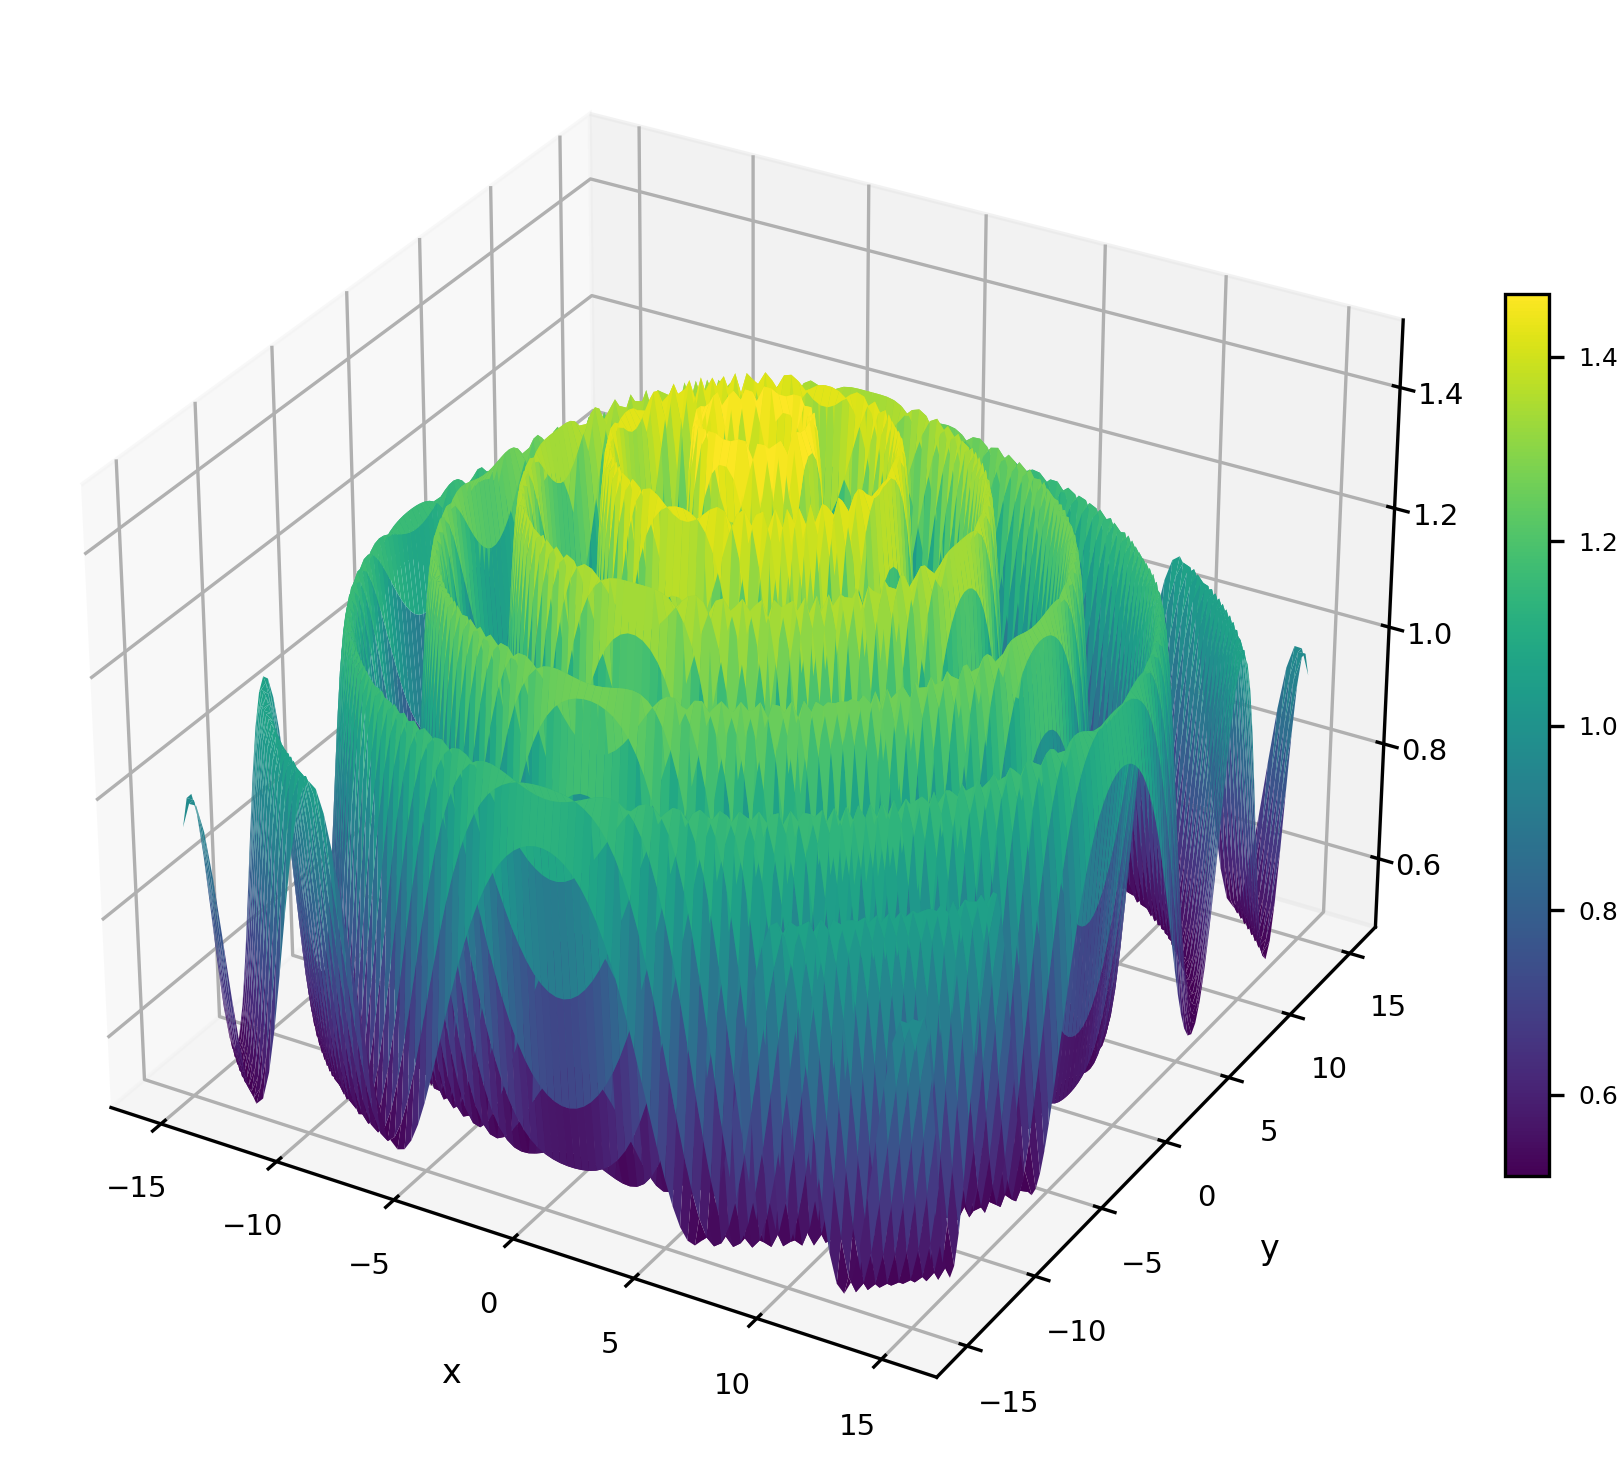
\includegraphics[width=1\textwidth]{Figures/benchmark_plots/SineEnvelope_maximized.png}
        \caption{Sine Envelope}
    \end{subfigure}
    \begin{subfigure}{0.32\textwidth}
        \centering
        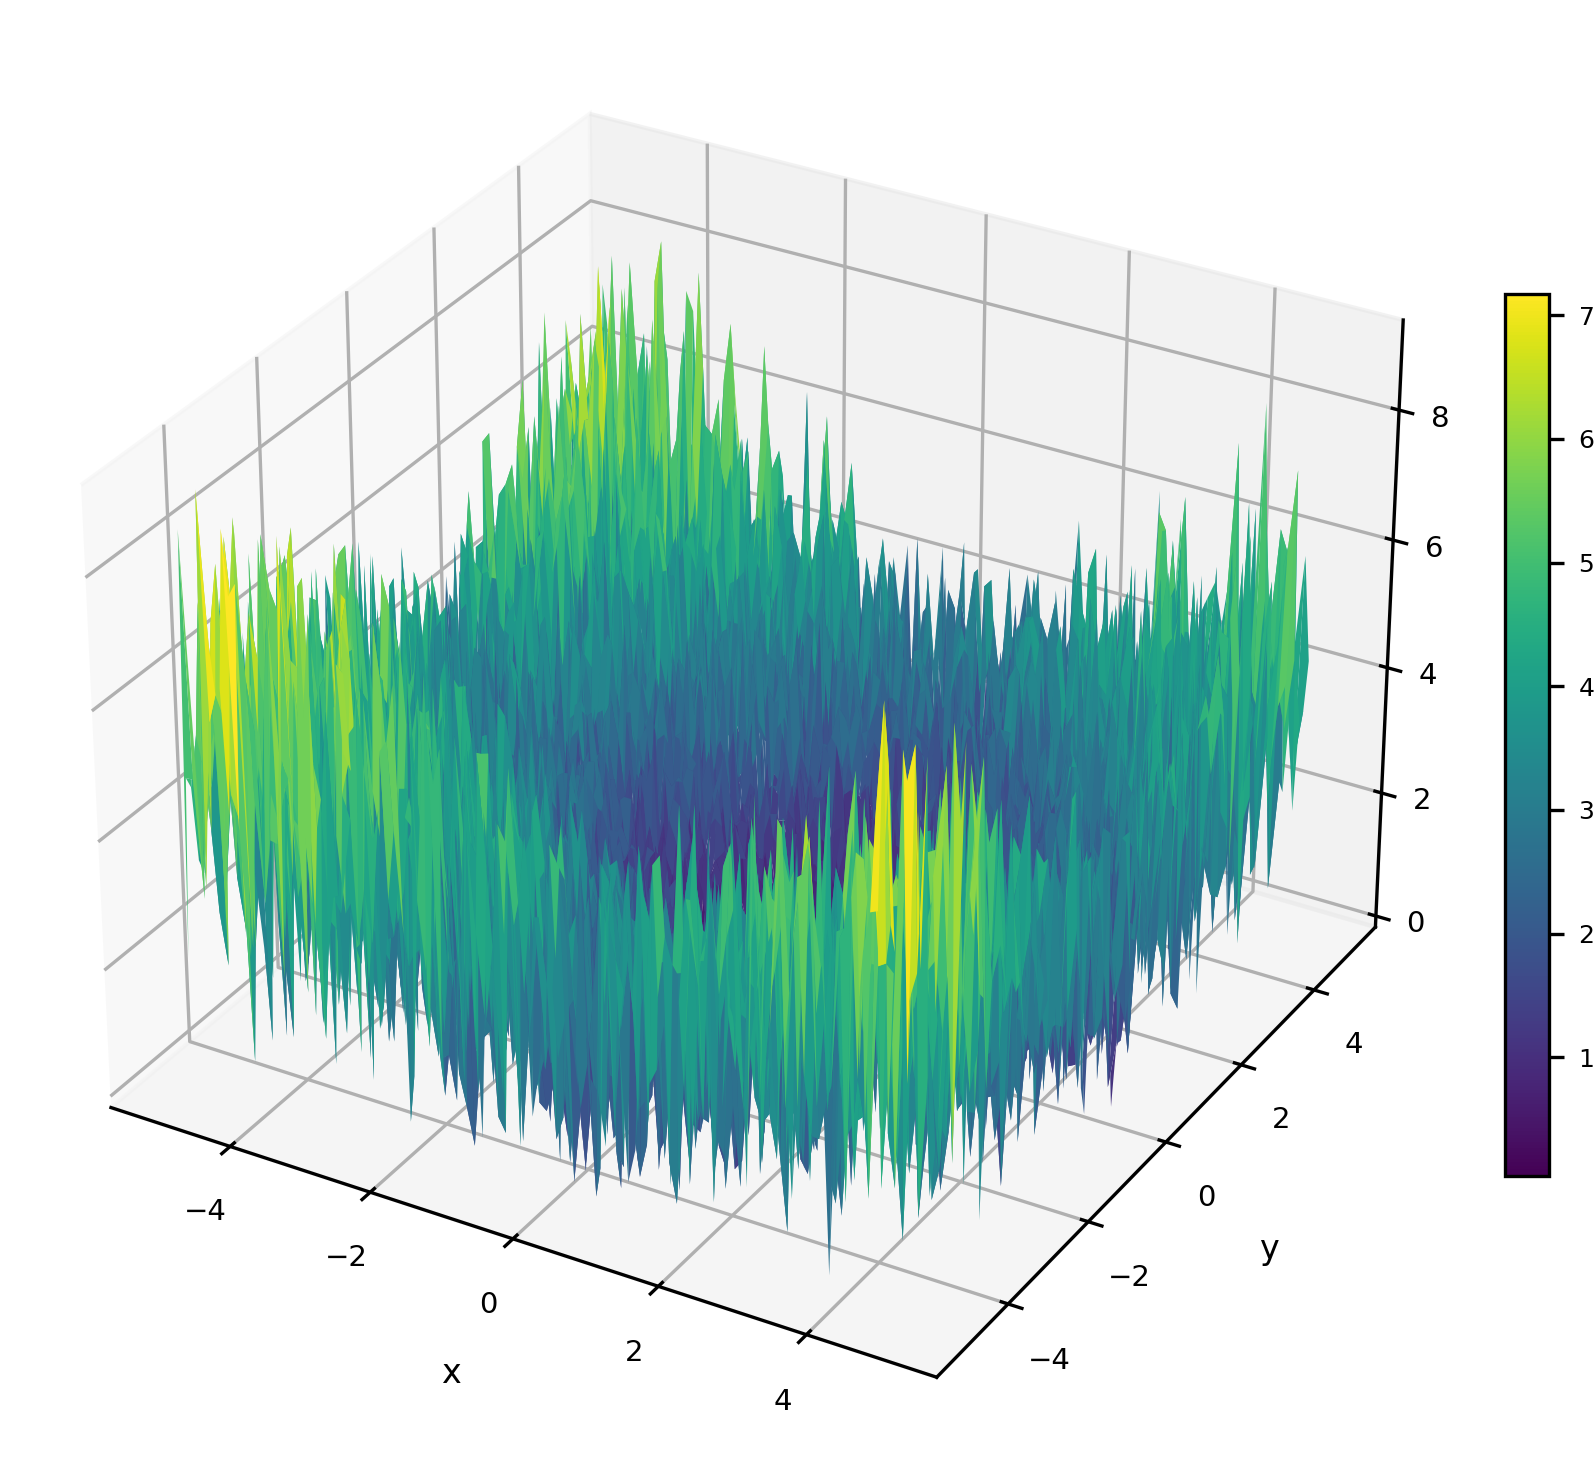
\includegraphics[width=1\textwidth]{Figures/benchmark_plots/Stochastic_maximized.png}
        \caption{Stochastic}
    \end{subfigure}
    % \hspace{.5cm} % Adjust the space as needed.
    \begin{subfigure}{0.32\textwidth}
        \centering
        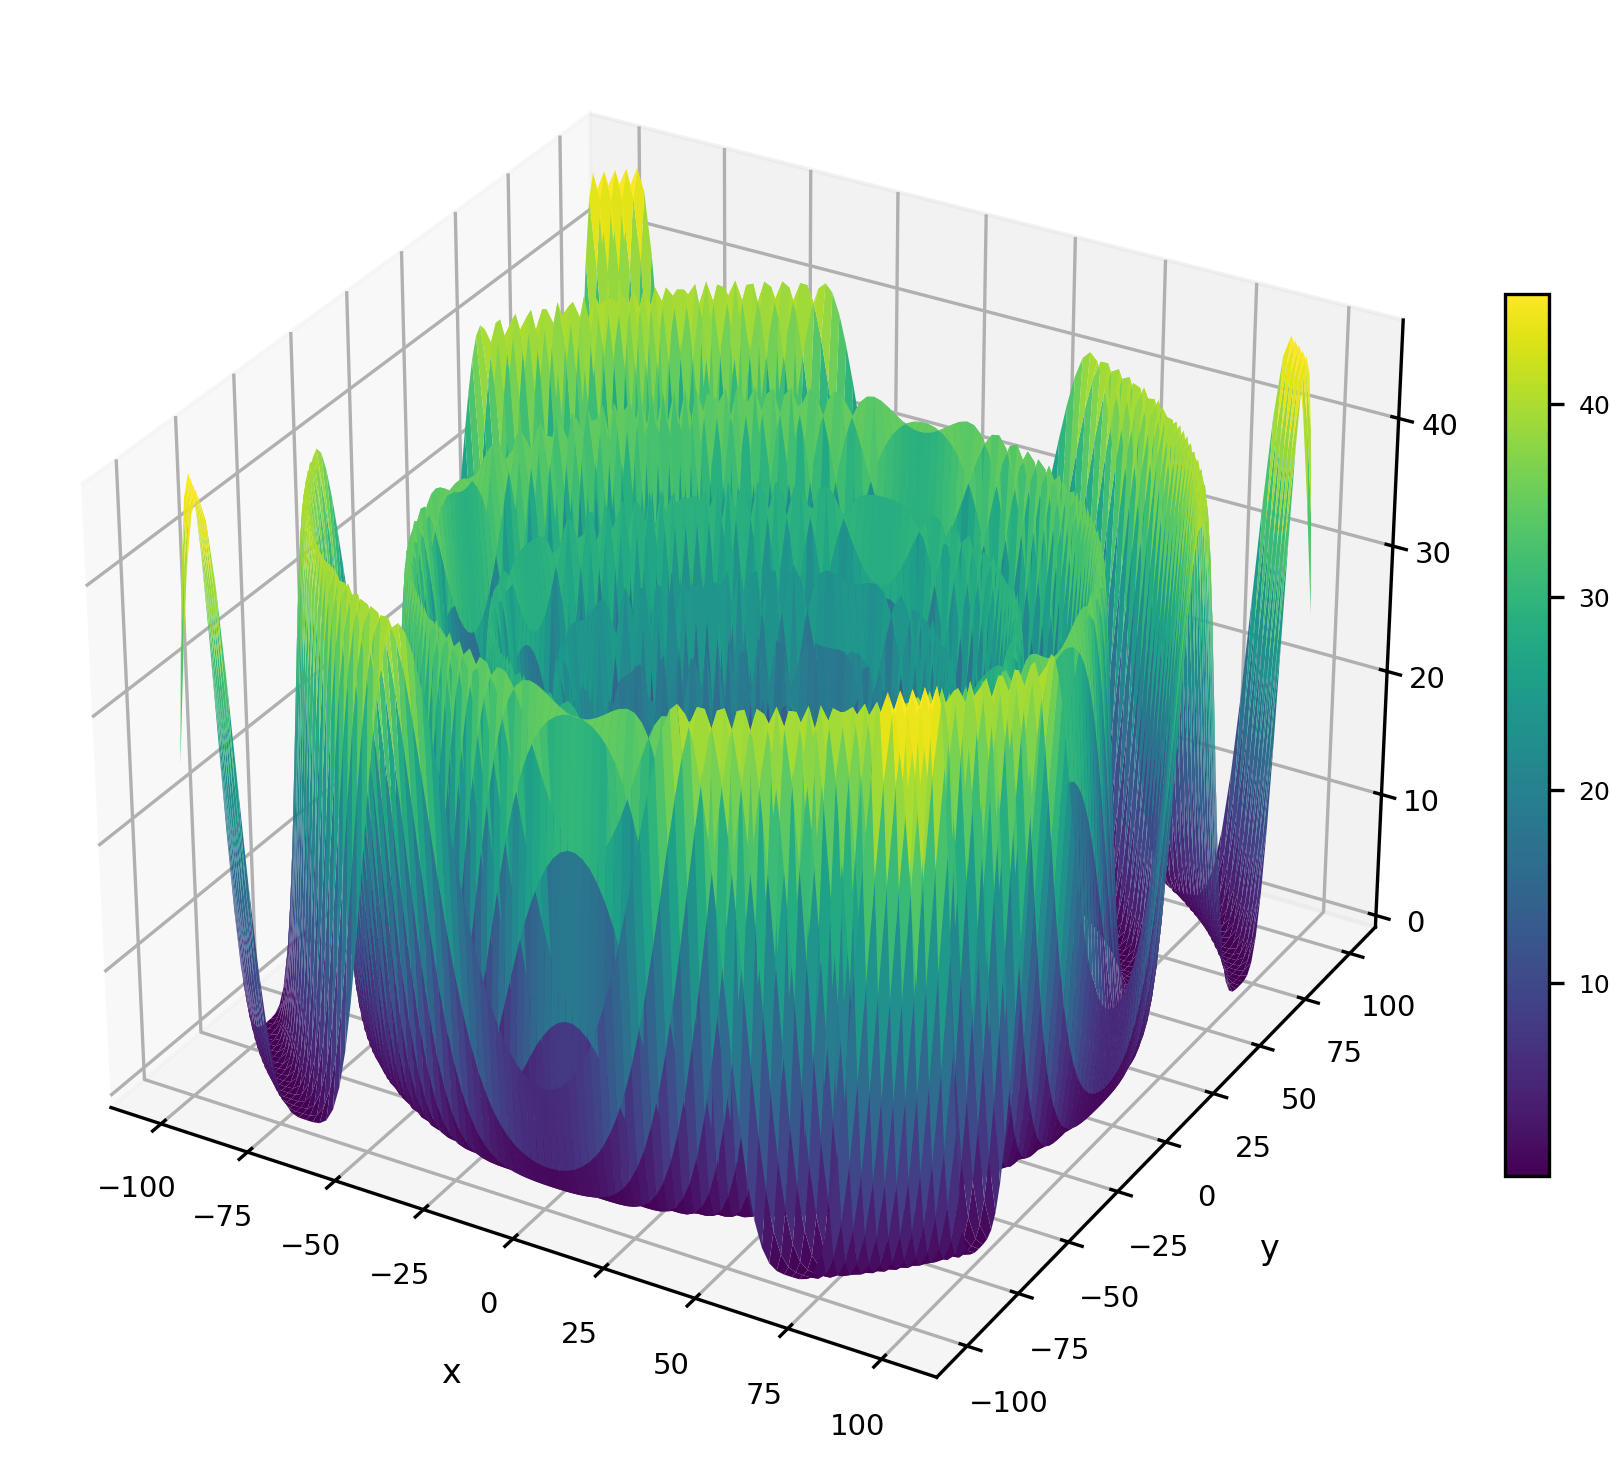
\includegraphics[width=1\textwidth]{Figures/benchmark_plots/StretchedV_maximized.png}
        \caption{Stretched V}
    \end{subfigure}
        \begin{subfigure}{0.32\textwidth}
        \centering
        \includegraphics[width=1\textwidth]{Figures/benchmark_plots/Styblinski–Tang_maximized.png}
        \caption{Styblinski–Tang}
    \end{subfigure}
        \captionsetup{list=no}
\caption{Two-dimensional visualizations of benchmark problem landscapes.}
\label{fig:benchmark_problems_plot}
\end{figure}